%\documentclass[handout]{beamer}
\documentclass{beamer}
\usepackage{comment}
\usepackage{multirow}
\usepackage{float}
\usepackage{fixltx2e}
\usepackage[boxed]{algorithm2e}
\SetAlFnt{\fontsize{7pt}{8pt}\selectfont \ttfamily}
\SetAlgoInsideSkip{} 
\renewcommand\AlCapFnt{\tiny}
\SetAlCapSkip{1.25ex}
\SetAlgoCaptionLayout{centering}
\setlength{\algomargin}{1.5em}
\SetInd{0.5em}{0.625em}
\usepackage{tikz}
\usepackage{pgfplots}
\usetikzlibrary{shapes.geometric,arrows,fit,matrix,positioning,pgfplots.groupplots}
\tikzset
{
    treenode/.style = {circle, draw=black, align=center, minimum size=1cm},
    subtree/.style  = {isosceles triangle, draw=black, align=center, minimum height=0.25cm, minimum width=0.25cm, shape border rotate=90, anchor=north},
    process/.style={rectangle, minimum width=2cm, minimum height=1cm, align=center, text width=2cm, draw},
    connector/.style={circle, minimum size=1cm, align=center, text width=0.5cm, draw},
    arrow/.style={thick, ->, >=stealth}
}
\usepackage{circuitikz}
\setbeamertemplate{caption}{\insertcaption}

\renewcommand\topfraction{0.95}
\renewcommand\bottomfraction{0.95}
\renewcommand\textfraction{0.05} 
\renewcommand\floatpagefraction{0.95}
\renewcommand{\dbltopfraction}{0.95}
\renewcommand{\dblfloatpagefraction}{0.95}	

\floatsep 4pt plus 2pt minus 2pt
\textfloatsep 8pt plus 2pt minus 4pt
\dblfloatsep 4pt plus 2pt minus 2pt
\dbltextfloatsep 8pt plus 2pt minus 4pt

\addtobeamertemplate{navigation symbols}{}{%
    \usebeamerfont{footline}%
    \usebeamercolor[fg]{footline}%
    \hspace{1em}%
    \insertframenumber/\inserttotalframenumber
}
\title{Concurrent Internal Binary Search Trees}
\author[Arun]{\includegraphics[height=0.8cm]{figures/utd_logo.jpg}\\
Arunmoezhi Ramachandran \\
Supervisor - Neeraj Mittal\\
}
\institute[UTDallas]{The University of Texas at Dallas}
\date{}
\begin{document}

\begin{frame}
	\titlepage
\end{frame}

		
\begin{frame}{Overview}
	\tableofcontents
\end{frame}

\section{Introduction}
With the growing prevalence of multi-core, multi-processor systems, concurrent data structures are becoming increasingly important. In such a data structure, multiple processes may need to operate on the data structure at the same time. Contention between different processes must be managed in such a way that all operations complete correctly and leave the data structure in a valid state.

Concurrency is often managed using locks. A lock can be used to achieve mutual exclusion, which can then be used to ensure that any updates to the data structure or a portion of it are performed by one process at a time. This makes it easier to design a lock-based concurrent data structure and reason about its correctness. Moreover, this also makes it easier to implement a lock-based data structure and debug it than its lock-free counterpart. Lock-based algorithms for concurrent versions of many important data structures for storing and managing shared data have been developed including linked lists, queues, priority queues, hash tables and skiplists (\emph{e.g.}, \cite{MicSco:1996:PODC, Mic:2002:SPAA,Lea:2003:JSR166,HelHer+:2005:OPODIS,LevHer+:2007:SIROCCO, HerSha:2012:Book}).

However, locks are blocking; while a process is holding a lock, no other process can access the portion of the data structure protected by the lock. If a process stalls while it is holding a lock, then the lock may not be released for a long time. This may cause other processes to wait on the stalled process for extended periods of time. As a result, lock-based implementations of concurrent data structures are vulnerable to problems such as deadlock, priority inversion and convoying~\cite{HerSha:2012:Book}.

Non-blocking algorithms avoid the pitfalls of locks by using special (hardware-supported) \emph{read-modify-write} instructions such as \emph{load-link/store-conditional (\LL{}/\SC{})}  and \linebreak \emph{compare-and-swap (\CAS{})}~\cite{HerSha:2012:Book}. Non-blocking implementations of many common data structures such as queues, stacks, linked lists, hash tables and search trees  have been proposed (\emph{e.g.}, \cite{Mic:2002:SPAA,FomRup:2004:PODC,BenFin+:2005:SPAA,EllFat+:2010:PODC,HerSha:2012:Book,BraPet:2012:SPAA,HowJon:2012:SPAA,NatMit:2013:DISC,NatSav+:2013:SSS,NatMit:2014:PPoPP,DraVec+:2014:PPoPP,EllFat+:2014:PODC}).

Binary search tree is one of the fundamental data structures for organizing \emph{ordered} data that supports search, insert and delete operations~\cite{CorLei+:1991:MIT}. A binary search tree may be unbalanced (different leaf nodes may be at very different depths) or balanced (all leaf nodes are at roughly the same depth). A balanced binary search tree provides better worst-case guarantees about the cost of performing an operation on the tree. However, in many cases, the overhead of keeping the tree balanced, especially in a concurrent environment, may incur significant overhead. As a result, in many cases, an unbalanced binary search tree  outperforms a balanced binary search tree in practice. In this work, our focus is on developing efficient concurrent algorithms for an \emph{unbalanced} binary search tree. 

Concurrent algorithms for unbalanced binary search trees have been proposed in~\cite{EllFat+:2010:PODC,HowJon:2012:SPAA,NatMit:2014:PPoPP,DraVec+:2014:PPoPP,EllFat+:2014:PODC,ChaDan+:2014:PODC,ArbAtt:2014:PODC}. Algorithms in~\cite{DraVec+:2014:PPoPP,ArbAtt:2014:PODC} are blocking (or lock-based), whereas those in~\cite{EllFat+:2010:PODC,HowJon:2012:SPAA,NatMit:2014:PPoPP,EllFat+:2014:PODC,ChaDan+:2014:PODC} are non-blocking (or lock-free). Also, algorithms in~\cite{HowJon:2012:SPAA,DraVec+:2014:PPoPP,ArbAtt:2014:PODC,ChaDan+:2014:PODC} use internal representation of a search tree in which all nodes store data, where as those in~\cite{EllFat+:2010:PODC,NatMit:2014:PPoPP,EllFat+:2014:PODC} use an external representation of  a search tree in which only leaf nodes store data (data stored in internal nodes is used for routing purposes only).

Algorithms that use internal representation of a search tree have to address the problem that arises due to a key moving from one location in the tree to another. This occurs when the key undergoing deletion resides in a binary node, which requires it to be either replaced with its predecessor (next smallest key) or its successor (next largest key). As a result, an operation traversing the tree may fail to find the target key both at its old location and at its new location, even though the target key was continuously present in the tree. Different algorithms use different approaches to handle the problem arising due to key movement. The algorithm by Drachsler \emph{et al.} in~\cite{DraVec+:2014:PPoPP} maintains a \emph{sorted} linked list of all the keys in the tree. If the traversal of the tree fails to find a given key, then an operation traverses the linked list to look for the key. The algorithm by Arbel and Hattiya~\cite{ArbAtt:2014:PODC} uses the RCU (Read-Copy-Update) framework (first employed in Linux kernels) to allow reads to occur concurrently with updates.

Most of the concurrent algorithms (for BSTs) that have proposed so far use a na{\"i}ve approach and simply restart the traversal from the root of the tree~\cite{EllFat+:2010:PODC,HowJon:2012:SPAA,NatMit:2014:PPoPP,DraVec+:2014:PPoPP,ArbAtt:2014:PODC}. This is especially undesirable if the tree has large height, and the overhead of repeatedly traversing the tree may dominate all other overheads of performing an operation.

Recently, a few algorithms have been proposed in which an operation attempts to recover from a failure \emph{locally}~\cite{EllFat+:2014:PODC,ChaDan+:2014:PODC}. The algorithm in~\cite{EllFat+:2014:PODC}, which is based on external representation and builds upon the algorithm in~\cite{EllFat+:2010:PODC}, maintains a stack of the nodes visited during the traversal of the tree and simply restarts from the last ``unmarked'' node  (a node is marked before it is removed from the tree). Intuitively, this works because, in an external search tree, keys \emph{do not} move from one location in the tree to another. However, in a search tree based on internal representation, keys may move from one location (in the tree) to another. This occurs when the key undergoing deletion resides in a binary node, which requires it to be either replaced with its predecessor (next smallest key) or its successor (next largest key). This causes two problems. First, an operation traversing the tree may fail to find the target key both at its old location and at its new location, even though the target key was continuously present in the tree. Second, it is not always safe to simply restart from the last unmarked node in the stack since the key may have moved to an ancestor of such a node. Their restart approach is, however, sufficiently general that it can be applied to other concurrent search trees based on external representation~\cite{NatMit:2014:PPoPP}.

The algorithm in~\cite{ChaDan+:2014:PODC},  which is based on internal representation, uses \emph{backlink pointers} to find its way and recover from a failure while executing an operation. Their restart approach appears to be customized for their concurrent search tree and is not clear how it can be extended to other concurrent search trees based on internal representation.

\section{Contributions}
First we present a new \emph{lock-based} algorithm for concurrent manipulation of a binary search tree in an asynchronous shared memory system that supports search, insert and delete operations. Our algorithm is based on an internal representation of a search tree as in~\cite{DraVec+:2014:PPoPP,ArbAtt:2014:PODC}. However, as in~\cite{NatMit:2014:PPoPP}, it operates at edge-level (locks edges) rather than at node-level (locks nodes); this minimizes the contention window of a write operation and improves the system throughput. 
%%
Further, in our algorithm, 
%%
\begin{enumerate*}[label=(\roman*)]
\item a search operation uses only read and write instructions, 
\item an insert operation does not acquire any locks, and
\item a delete operation only needs to lock up to four edges in the absence of contention.
\end{enumerate*}
%%
Our experiments indicate that our lock-based algorithm outperforms existing algorithms for a concurrent binary search 
tree---blocking as well as non-blocking---for medium-sized and larger trees, achieving up to \castleMaximumgap{} higher throughput than the next best algorithm.

Second we extend the previous algorithm to develop a new \emph{lock-free} algorithm. It combines ideas from two existing lock-free algorithms, namely those by Howley and Jones~\cite{HowJon:2012:SPAA} and Natarajan and Mittal~\cite{NatMit:2014:PPoPP}, and is especially \emph{optimized for the conflict-free scenario}. Like Howley and Jones' algorithm, it uses internal representation of a search tree in which all nodes store keys. Also, like Natarajan and Mittal's algorithm, it operates at edge-level rather than node-level and does not use a separate explicit object for enabling coordination among conflicting operations. As a result, it inherits benefits of both the lock-free algorithms. Specifically, when compared to modify operations of Howley and Jones' internal binary search tree, its modify operations 
\begin{enumerate*}[label=(\alph*)]
\item have a smaller contention window, 
\item allocate fewer objects, 
\item execute fewer atomic instructions, and 
\item have a smaller memory footprint. 
\end{enumerate*}
%%
Our experiments indicate that our new lock-free algorithm outperforms other lock-free algorithms in most cases, providing up to \icdcnMaximumgap{} improvement in some cases over the next best algorithm.

Third, we present a general approach for local recovery that enables a process to quickly recover from a failure while performing an operation by restarting the traversal from a point ``close'' to the operation's window rather than the root of the tree.  Our approach can be applied to many existing concurrent algorithms for maintaining binary search trees using internal representation---blocking as well as non-blocking---such as those in~\cite{HowJon:2012:SPAA,DraVec+:2014:PPoPP,ArbAtt:2014:PODC,RamMit:2015:PPoPP}. Our local recovery approach uses only local variables and does not require modifying a tree node (of the original algorithm) to store any additional information. Using experimental evaluation, we demonstrate that our local recovery approach can yield significant speed-ups for many concurrent algorithms.

Finally, we present two light-weight techniques to make search operations for concurrent binary search trees based on internal representation, such as those in those in~\cite{HowJon:2012:SPAA,DraVec+:2014:PPoPP,ArbAtt:2014:PODC,RamMit:2015:ICDCN,RamMit:2015:PPoPP}, \emph{wait-free} with low additional overhead. Both of our techniques have the desirable feature that a search operation does not need to perform any write instructions on the share memory thereby minimizing the cache coherence traffic.

\section{Dissertation Roadmap} 
This dissertation organized as follows. We first describe the key concepts and techniques related to concurrent data structures in \chapterref{\preliminaries}. Then we describe our lock-based algorithm for a binary search tree in \chapterref{castle} followed by our lock-free algorithm in \chapterref{icdcn}. Our general technique for local recovery is described in \chapterref{localRecovery}. Then we discuss \emph{wait-free} techniques for search operations in \chapterref{waitFreeSearch}. The experimental evaluation of different concurrent algorithms for a binary search tree is described in \chapterref{experiments}. Finally \chapterref{conclusion} concludes the dissertation and outlines directions for future research.

\section{Design Approaches}
\begin{frame}{Designing Concurrent Data Structures}
\begin{itemize}
\item Shared-memory multiprocessors concurrently execute multiple threads
\item Threads communicate and synchronize through data structures in shared memory
\item Threads can interleave in exponential number of ways
\item Concurrent data structure must preserve its properties for all possible interleavings
\end{itemize}
\end{frame}

\begin{frame}{Example - Shared Counter}
Let $x$ be a shared counter which can be incremented using a function fetchAndIncrement()\\
\pause
Here are some possible implementations of this function\\
\phantom{hello world}
\SetAlgorithmName{fetchAndIncrement}{}{}
\renewcommand{\thealgocf}{}
\begin{minipage}[t]{0.48\textwidth}
\begin{algorithm}[H]
\phantom{acquire(lock)\;}
r1 = x\;
inc(r1)\;
x = r1\;
\phantom{release(lock)\;}

\caption{\tiny sequential}
\end{algorithm}
\pause
\end{minipage}
\begin{minipage}[t]{0.48\textwidth}
\begin{algorithm}[H]
\caption{\tiny Using locks}
acquire(lock)\;
r1 = x\;
inc(r1)\;
x = r1\;
release(lock)\;

\end{algorithm}
\end{minipage}
\pause
\begin{center}
\begin{minipage}[t]{0.65\textwidth}
\begin{algorithm}[H]
\caption{\tiny using atomic instructions}
\Repeat{(x.compareAndSwap(rOld,rNew))}
{
rOld = x\;
rNew = rOld+1\;
}
\end{algorithm}
\end{minipage}
\end{center}
\footnotesize compareAndSwap updates(atomically) the value of $x$ to $rNew$ only if the read value of $x$ is equal to $rOld$. Returns \textit{true} if it succeeds in updating the value of $x$
\end{frame}

\begin{frame}{Design Approaches}
\begin{center}
\Large How to handle contention among threads?
\end{center}
\pause
\begin{itemize}
\item<2-> \Large Blocking Algorithms
\begin{itemize}
\item<3-> use locks to resolve contention
\item<3-> coarse grained or fine grained locking
\item<3->  {\color{black!50!green} easier to design}
\item<3->  {\color{red}weaker progress guarantees} (thread owns a lock) 
\item<3->  {\color{red}are prone to deadlock, priority inversion}
\end{itemize}
\phantom{hello world}
\item<2-> \Large Non-Blocking Algorithms
\begin{itemize}
\item<4->  use atomic (Read-Modify-Write) instructions to resolve contention. E.g. Compare-And-Swap(CAS) instruction
\item<4-> lock-free or wait-free
\item<4-> {\color{black!50!green}stronger progress guarantees} (operation owns a lock - helping)
\item<4-> {\color{black!50!green}deadlock or priority inversion not possible}
\item<4-> {\color{red}harder to design}
\end{itemize}
\end{itemize}
\end{frame}

\section{Linearizability}
\begin{figure}[htp]
	\subcaptionbox{Sequential}[0.45\textwidth]
	{
		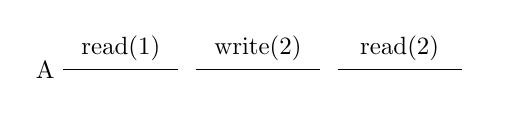
\begin{tikzpicture}[scale=0.9, transform shape] 
		\node (x1)  {A};
		\node (x2) [right of=x1,xshift=1cm]{};
		\draw (x1) -- node[above]{read(1)} (x2);
		\node(x3)[right of=x2,xshift=-1cm]{};
		\node(x4) [right of=x3,xshift=1cm]{};
		\draw (x3) -- node[above]{write(2)} (x4);
		
		\node(x5)[right of=x4,xshift=-1cm]{};
		\node(x6) [right of=x5,xshift=1cm]{};
		\draw (x5) -- node[above]{read(2)} (x6);
		\end{tikzpicture}
	}
	%\quad
	\subcaptionbox{Concurrent - linearizable}[0.45\textwidth]
	{
		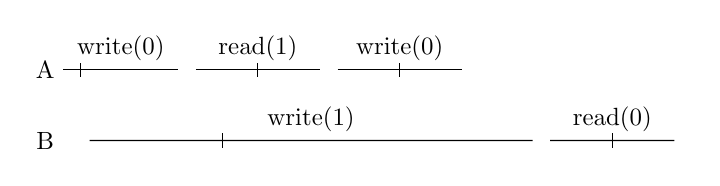
\begin{tikzpicture}[scale=0.9, transform shape] 
		\node (x1) {A};
		\node (x2) [right of=x1,xshift=1cm]{};
		\draw (x1) -- node[above]{write(0)} (x2);
		\draw (0.5,-0.1) -- (0.5,+0.1);
		
		\node(x3)[right of=x2,xshift=-1cm]{};
		\node(x4) [right of=x3,xshift=1cm]{};
		\draw (x3) -- node[above]{read(1)} (x4);
		\draw (3,-0.1) -- (3,+0.1);
		
		\node(x5)[right of=x4,xshift=-1cm]{};
		\node(x6) [right of=x5,xshift=1cm]{};
		\draw (x5) -- node[above]{write(0)} (x6);
		\draw (5,-0.1) -- (5,+0.1);
		
		\node(B)[below of=x1]{B};
		\node(x7)[below of=x1,xshift=0.5cm]{};
		\node(x8) [right of=x7,xshift=5.5cm]{};
		\draw (x7) -- node[above]{write(1)} (x8);
		\draw (2.5,-1.1) -- (2.5,-0.9);
		
		\node(x9)[right of=x8,xshift=-1cm]{};
		\node(x10) [right of=x9,xshift=1cm]{};
		\draw (x9) -- node[above]{read(0)} (x10);
		\draw (8,-1.1) -- (8,-0.9);
		
		\end{tikzpicture}
	}
%%%%%%%%%%%%%%
\\
%%%%%%%%%%%%%%
%%%%%%%%%%%%%%
\\
%%%%%%%%%%%%%%
\begin{center}
	\subcaptionbox{Concurrent - not linearizable}
	{
		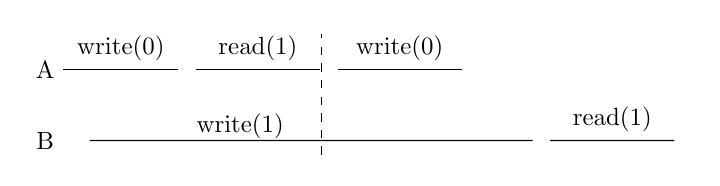
\begin{tikzpicture}[scale=0.9, transform shape] 
		\node (x1) {A};
		\node (x2) [right of=x1,xshift=1cm]{};
		\draw (x1) -- node[above]{write(0)} (x2);
		
		\node(x3)[right of=x2,xshift=-1cm]{};
		\node(x4) [right of=x3,xshift=1cm]{};
		\draw (x3) -- node[above]{read(1)} (x4);
		\draw[dashed] (3.9,-1.2) -- (3.9,+0.5);
		
		\node(x5)[right of=x4,xshift=-1cm]{};
		\node(x6) [right of=x5,xshift=1cm]{};
		\draw (x5) -- node[above]{write(0)} (x6);
		
		\node(B)[below of=x1]{B};
		\node(x7)[below of=x1,xshift=0.5cm]{};
		\node(x8) [right of=x7,xshift=5.5cm]{};
		\draw (x7) -- node [above, xshift=-1cm,yshift=-0.1cm] {write(1)} (x8);
		
		\node(x9)[right of=x8,xshift=-1cm]{};
		\node(x10) [right of=x9,xshift=1cm]{};
		\draw (x9) -- node[above]{read(1)} (x10);
		
		\end{tikzpicture}
	}
	\caption{A sample history of an object \label{fig:linearizability}}
\end{center}
\end{figure}

\section{Binary Search Tree}
\begin{frame}{Binary Search Tree - Defintion}
A \textit{binary search tree} (BST) is a data structure which meets the following requirements:
\begin{itemize}
\item it  is a binary tree (a node can contain atmost two children)
\item each node contains a key $k$
\item left subtree of a node contains keys lesser than $k$
\item right subtree of a node contains keys greater than $k$
\end{itemize}
\pause
Operations on a BST
\begin{itemize}
\item \textbf{search($k$)} - returns \textit{true} only if key $k$ is present in the tree
\item \textbf{insert($k$)} - inserts $k$ into the tree if it does not already exist
\item \textbf{delete($k$)} - deletes $k$ from the tree if it already exist
\end{itemize}
\end{frame}

\begin{frame}{BST - Search}
\textbf{search($70$)}\\
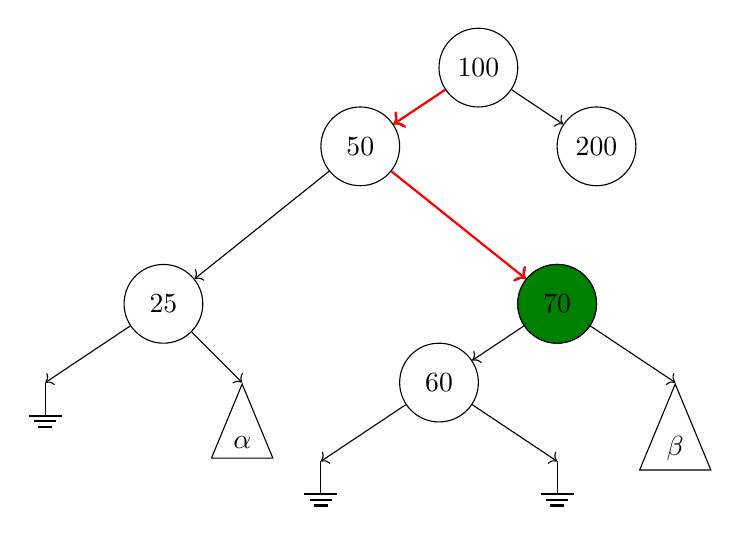
\begin{tikzpicture}
\newcommand\xShift{1.5}
\newcommand\yShift{1}
\node(x) [treenode] at (0, 0) {100};
\node(xl) [treenode] at ([shift=({-\xShift,-\yShift})]x) {50};
\node(xr) [treenode] at ([shift=({\xShift,-\yShift})]x) {200};
\node(xll) [treenode] at ([shift=({-\xShift-1,-\yShift-1})]xl) {25};
\node(xlr) [treenode] at ([shift=({\xShift+1,-\yShift-1})]xl) {70};
\node(xlll) [ground] at ([shift=({-\xShift,-\yShift})]xll) {};
\node(xllr) [subtree] at ([shift=({\xShift-0.5,-\yShift})]xll) {$\alpha$};
\node(xlrl) [treenode] at ([shift=({-\xShift,-\yShift})]xlr) {60};
\node(xlrr) [subtree] at ([shift=({\xShift,-\yShift})]xlr) {$\beta$};
\node(xlrll) [ground] at ([shift=({-\xShift,-\yShift})]xlrl) {};
\node(xlrlr) [ground] at ([shift=({\xShift,-\yShift})]xlrl) {};
\draw[->] (x) -- (xl);
\draw[->] (x) -- (xr);
\draw[->] (xl) -- (xll);
\draw[->] (xl) -- (xlr);
\draw[->] (xll) -- (xlll);
\draw[->] (xll) -- (xllr.north);
\draw[->] (xlr) -- (xlrl);
\draw[->] (xlr) -- (xlrr.north);
\draw[->] (xlrl) -- (xlrll);
\draw[->] (xlrl) -- (xlrlr);
\draw<2->[->,thick,color=red] (x) -- (xl);
\draw<3->[->,thick,color=red] (xl) -- (xlr);
\node<4->(xlr) [treenode,fill=black!50!green] at ([shift=({\xShift+1,-\yShift-1})]xl) {70};
\end{tikzpicture}
\end{frame}

\begin{frame}{BST - Search}
\textbf{search($55$)}\\
\input{figures/BST/searchFalse}
\end{frame}

\begin{frame}{BST - Insert}
\textbf{insert($55$)}\\
\begin{columns}
\begin{column}[t]{0.48\textwidth}
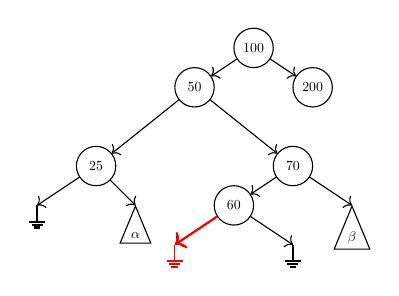
\begin{tikzpicture}[scale=0.5, transform shape]
\newcommand\xShift{1.5}
\newcommand\yShift{1}
\node(x) [treenode] at (0, 0) {100};
\node(xl) [treenode] at ([shift=({-\xShift,-\yShift})]x) {50};
\node(xr) [treenode] at ([shift=({\xShift,-\yShift})]x) {200};
\node(xll) [treenode] at ([shift=({-\xShift-1,-\yShift-1})]xl) {25};
\node(xlr) [treenode] at ([shift=({\xShift+1,-\yShift-1})]xl) {70};
\node(xlll) [ground] at ([shift=({-\xShift,-\yShift})]xll) {};
\node(xllr) [subtree] at ([shift=({\xShift-0.5,-\yShift})]xll) {$\alpha$};
\node(xlrl) [treenode] at ([shift=({-\xShift,-\yShift})]xlr) {60};
\node(xlrr) [subtree] at ([shift=({\xShift,-\yShift})]xlr) {$\beta$};
\node(xlrll) [ground] at ([shift=({-\xShift,-\yShift})]xlrl) {};
\node(xlrlr) [ground] at ([shift=({\xShift,-\yShift})]xlrl) {};
\draw[->] (x) -- (xl);
\draw[->] (x) -- (xr);
\draw[->] (xl) -- (xll);
\draw[->] (xl) -- (xlr);
\draw[->] (xll) -- (xlll);
\draw[->] (xll) -- (xllr.north);
\draw[->] (xlr) -- (xlrl);
\draw[->] (xlr) -- (xlrr.north);
\draw[->] (xlrl) -- (xlrll);
\draw[->] (xlrl) -- (xlrlr);
\draw<2->[->,thick,color=red] (xlrl) -- (xlrll);
\node<2->(xlrll) [ground,color=red] at ([shift=({-\xShift,-\yShift})]xlrl) {};
\end{tikzpicture}
\end{column}
\pause
\pause
\begin{column}[t]{0.5\textwidth}
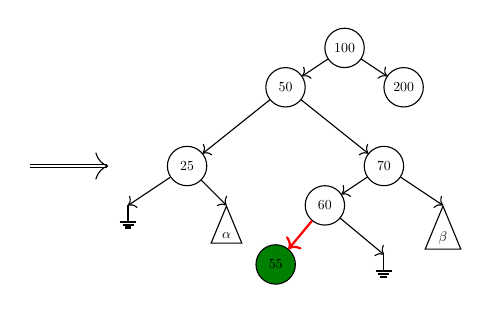
\begin{tikzpicture}[scale=0.5, transform shape]
\draw[->,style=double] (-8,-3) -- (-6,-3){};
\newcommand\xShift{1.5}
\newcommand\yShift{1}
\node(x) [treenode] at (0, 0) {100};
\node(xl) [treenode] at ([shift=({-\xShift,-\yShift})]x) {50};
\node(xr) [treenode] at ([shift=({\xShift,-\yShift})]x) {200};
\node(xll) [treenode] at ([shift=({-\xShift-1,-\yShift-1})]xl) {25};
\node(xlr) [treenode] at ([shift=({\xShift+1,-\yShift-1})]xl) {70};
\node(xlll) [ground] at ([shift=({-\xShift,-\yShift})]xll) {};
\node(xllr) [subtree] at ([shift=({\xShift-0.5,-\yShift})]xll) {$\alpha$};
\node(xlrl) [treenode] at ([shift=({-\xShift,-\yShift})]xlr) {60};
\node(xlrr) [subtree] at ([shift=({\xShift,-\yShift})]xlr) {$\beta$};
\node(xlrll) [treenode,fill=black!50!green] at ([shift=({-\xShift+0.25,-\yShift-0.5})]xlrl) {55};
\node(xlrlr) [ground] at ([shift=({\xShift,-\yShift-0.25})]xlrl) {};
\draw[->] (x) -- (xl);
\draw[->] (x) -- (xr);
\draw[->] (xl) -- (xll);
\draw[->] (xl) -- (xlr);
\draw[->] (xll) -- (xlll);
\draw[->] (xll) -- (xllr.north);
\draw[->] (xlr) -- (xlrl);
\draw[->] (xlr) -- (xlrr.north);
\draw[->,thick,color=red] (xlrl) -- (xlrll);
\draw[->] (xlrl) -- (xlrlr);
\end{tikzpicture}
\end{column}
\end{columns}
\end{frame}

\begin{frame}{Types of delete}
\begin{itemize}
\item simple - removing a node which has atmost one child
\item complex - removing a node which has exactly two children
\end{itemize}
\end{frame}

\begin{frame}{BST - Simple Delete}
\textbf{delete($25$)}
\begin{figure}[b]
\begin{columns}
\begin{column}[t]{0.48\textwidth}
\input{figures/BST/simpleDeleteA}
\end{column}
\pause
\pause
\begin{column}[t]{0.5\textwidth}
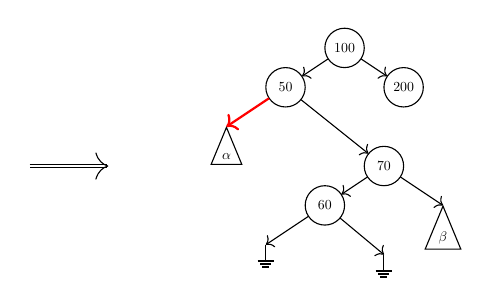
\begin{tikzpicture}[scale=0.5, transform shape]
\draw[->,style=double] (-8,-3) -- (-6,-3){};
\newcommand\xShift{1.5}
\newcommand\yShift{1}
\node(x) [treenode] at (0, 0) {100};
\node(xl) [treenode] at ([shift=({-\xShift,-\yShift})]x) {50};
\node(xr) [treenode] at ([shift=({\xShift,-\yShift})]x) {200};
\node(xll) [subtree] at ([shift=({-\xShift,-\yShift})]xl) {$\alpha$};
\node(xlr) [treenode] at ([shift=({\xShift+1,-\yShift-1})]xl) {70};
\node(xlrl) [treenode] at ([shift=({-\xShift,-\yShift})]xlr) {60};
\node(xlrr) [subtree] at ([shift=({\xShift,-\yShift})]xlr) {$\beta$};
\node(xlrll) [ground] at ([shift=({-\xShift,-\yShift})]xlrl) {};
\node(xlrlr) [ground] at ([shift=({\xShift,-\yShift-0.25})]xlrl) {};
\draw[->] (x) -- (xl);
\draw[->] (x) -- (xr);
\draw[->,thick,color=red] (xl) -- (xll.north);
\draw[->] (xl) -- (xlr);
\draw[->] (xlr) -- (xlrl);
\draw[->] (xlr) -- (xlrr.north);
\draw[->] (xlrl) -- (xlrll);
\draw[->] (xlrl) -- (xlrlr);
\end{tikzpicture}
\end{column}
\end{columns}
\end{figure}
\end{frame}

\begin{frame}{BST - Complex Delete}
\textbf{delete($50$)}
\begin{figure}[b]
\begin{columns}
\begin{column}[t]{0.33\textwidth}
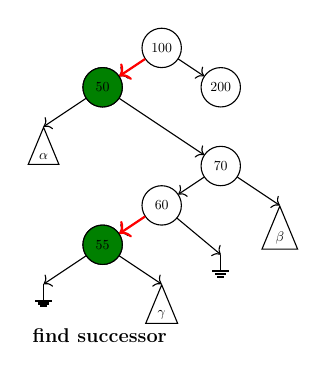
\begin{tikzpicture}[scale=0.5, transform shape]
\newcommand\xShift{1.5}
\newcommand\yShift{1}
\node(x) [treenode] at (0, 0) {100};
\node(xl) [treenode] at ([shift=({-\xShift,-\yShift})]x) {50};
\node(xr) [treenode] at ([shift=({\xShift,-\yShift})]x) {200};
\node(xll) [subtree] at ([shift=({-\xShift,-\yShift})]xl) {$\alpha$};
\node(xlr) [treenode] at ([shift=({\xShift+1.5,-\yShift-1})]xl) {70};
\node(xlrl) [treenode] at ([shift=({-\xShift,-\yShift})]xlr) {60};
\node(xlrr) [subtree] at ([shift=({\xShift,-\yShift})]xlr) {$\beta$};
\node(xlrll) [treenode] at ([shift=({-\xShift,-\yShift})]xlrl) {55};
\node(xlrlr) [ground] at ([shift=({\xShift,-\yShift-0.25})]xlrl) {};
\node(xlrlll) [ground] at ([shift=({-\xShift,-\yShift})]xlrll) {};
\node(xlrllr) [subtree] at ([shift=({\xShift,-\yShift})]xlrll) {$\gamma$};
\draw[->] (x) -- (xl);
\draw[->] (x) -- (xr);
\draw[->] (xl) -- (xll.north);
\draw[->] (xl) -- (xlr);
\draw[->] (xlr) -- (xlrl);
\draw[->] (xlr) -- (xlrr.north);
\draw[->] (xlrl) -- (xlrll);
\draw[->] (xlrl) -- (xlrlr);
\draw[->] (xlrll) -- (xlrlll);
\draw[->] (xlrll) -- (xlrllr.north);
\draw<2->[->,thick,color=red] (x) -- (xl);
\node<2->(xl) [treenode,fill=black!50!green] at ([shift=({-\xShift,-\yShift})]x) {50};
\draw<3->[->,thick,color=red] (xlrl) -- (xlrll);
\node<3->(xlrll) [treenode,fill=black!50!green] at ([shift=({-\xShift,-\yShift})]xlrl) {55};
\node<3->[below right] at (current bounding box.south west) {\Large \textbf{find successor}};
\end{tikzpicture}
\end{column}
\pause
\pause
\pause
\begin{column}[t]{0.33\textwidth}
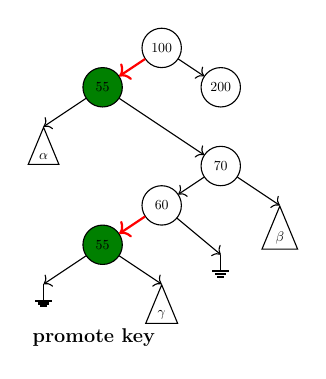
\begin{tikzpicture}[scale=0.5, transform shape]
%\draw[->,style=double] (-8,-3) -- (-7,-3){};
\newcommand\xShift{1.5}
\newcommand\yShift{1}
\node(x) [treenode] at (0, 0) {100};
\node(xl) [treenode,fill=black!50!green] at ([shift=({-\xShift,-\yShift})]x) {55};
\node(xr) [treenode] at ([shift=({\xShift,-\yShift})]x) {200};
\node(xll) [subtree] at ([shift=({-\xShift,-\yShift})]xl) {$\alpha$};
\node(xlr) [treenode] at ([shift=({\xShift+1.5,-\yShift-1})]xl) {70};
\node(xlrl) [treenode] at ([shift=({-\xShift,-\yShift})]xlr) {60};
\node(xlrr) [subtree] at ([shift=({\xShift,-\yShift})]xlr) {$\beta$};
\node(xlrll) [treenode,fill=black!50!green] at ([shift=({-\xShift,-\yShift})]xlrl) {55};
\node(xlrlr) [ground] at ([shift=({\xShift,-\yShift-0.25})]xlrl) {};
\node(xlrlll) [ground] at ([shift=({-\xShift,-\yShift})]xlrll) {};
\node(xlrllr) [subtree] at ([shift=({\xShift,-\yShift})]xlrll) {$\gamma$};
\draw[->,thick,color=red] (x) -- (xl);
\draw[->] (x) -- (xr);
\draw[->] (xl) -- (xll.north);
\draw[->] (xl) -- (xlr);
\draw[->] (xlr) -- (xlrl);
\draw[->] (xlr) -- (xlrr.north);
\draw[->,thick,color=red] (xlrl) -- (xlrll);
\draw[->] (xlrl) -- (xlrlr);
\draw[->] (xlrll) -- (xlrlll);
\draw[->] (xlrll) -- (xlrllr.north);
\node[below right] at (current bounding box.south west) {\Large \textbf{promote key}};
\end{tikzpicture}
\end{column}
\pause
\begin{column}[t]{0.33\textwidth}
\input{figures/BST/complexDeleteC}
\end{column}
\end{columns}
\end{figure}
\end{frame}

\section{Related Works}
\begin{comment}
\begin{frame}{Related Works}
\begin{itemize}
\item lock-free(node-based) external BST by Ellen et.al[PODC'10]
\item lock-free(node-based) internal BST by Howley and Jones[SPAA'12]
\item lock-free(edge-based) external BST by Natarajan and Mittal[PPoPP'14]
\item RCU-based(node-based) internal BST by Arbel and Attiya[PODC'14]
\item lock-based(node-based) internal BST by Drachsler et.al[PPoPP'14]
\end{itemize}
\end{frame}
\end{comment}
\begin{frame}{Related Works}
\begin{table}[h]
\small{
\begin{tabular}{|l|l|c|c|l|}
\hline
\textbf{\#} & \multicolumn{1}{c|}{\textbf{\begin{tabular}[c]{@{}c@{}}Algorithm\\ Type\end{tabular}}} & \textbf{\begin{tabular}[c]{@{}c@{}}Works\\ At\end{tabular}} & \textbf{\begin{tabular}[c]{@{}c@{}}BST\\ Type\end{tabular}} & \multicolumn{1}{c|}{\textbf{Authors}} \\ \hline
1           & lock free                                                                              & node level                                                  & external                                                    & Ellen et.al{[}PODC'10{]}              \\ \hline
2           & lock free                                                                              & node level                                                  & internal                                                    & Howley \& Jones{[}SPAA'12{]}          \\ \hline
3           & lock free                                                                              & edge level                                                  & external                                                    & Natarajan \&Mittal{[}PPoPP'14{]}      \\ \hline
4           & lock based                                                                             & node level                                                  & internal                                                    & Arbel \& Attiya{[}PODC'14{]}          \\ \hline
5           & lock based                                                                             & node level                                                  & internal                                                    & Drachsler et.al{[}PPoPP'14{]}         \\ \hline
\end{tabular}
}
\end{table}
\end{frame}

\section{Lock Based Binary Search Tree}
\begin{frame}[c]{Lock Based BST[PPoPP'15 Poster]}
Contributions
\begin{itemize}
\item combine edge-based locking with internal representation of BST
\item optimistic tree traversal 
\end{itemize}
\end{frame}

\begin{frame}[c]{Lock Based BST[PPoPP'15 Poster]}
\begin{itemize}
\item common workloads have more searches than updates
\begin{itemize}
\item design is optimized for searches
\item search operations are oblivious to locks
\end{itemize}
\pause
\item Any real life workload will have more inserts than deletes
\begin{itemize}
\item insert operations do not obtain any locks
\item performs only one atomic operation
\end{itemize}
\pause
\item removal of a node in a concurrent BST is challenging
\begin{itemize}
\item delete operations uses locks
\item locks can be obtained on nodes or edges
\item locking edges instead of nodes increases concurrency
\end{itemize}
\end{itemize}
\end{frame}

\begin{frame}{Lock Based BST - Challenges in search}
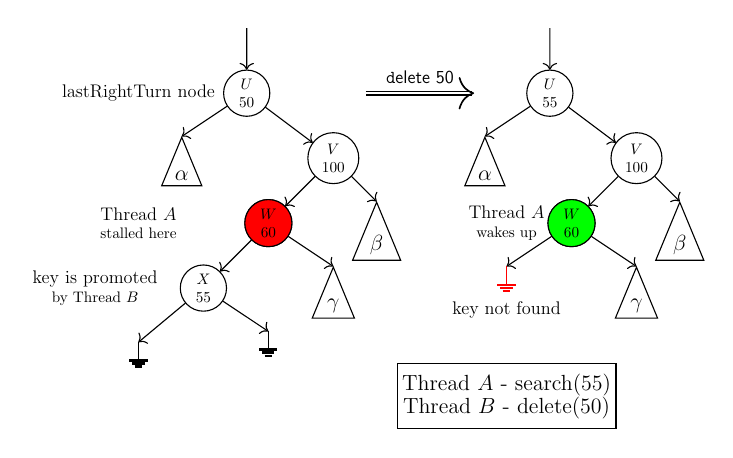
\begin{tikzpicture}[scale=0.55, transform shape,mylabel/.style={thin, draw=black, align=center, minimum width=0.3cm, minimum height=0.3cm,fill=white}]
		\newcommand\XA{0}
		\newcommand\YA{0}
		\node (x)		[treenode] 									at (-6,0)       							{$U$ \\ 50};
		\node (a)		[subtree] 									at (-7.5,-1)  								{\Large $\alpha$};
		\node (y0)	[treenode] 									at (-4,-1.5) 									{$V$ \\ 100};
		\node (y1)	[treenode]									at (-5.5,-3)									{$W$ \\ 60}; 
		\node (b)		[subtree] 									at (-3,-2.5)    							{\Large $\beta$};
		\node (y2)	[treenode]									at (-7,-4.5)									{$X$ \\ 55}; 
		\node (g)		[subtree] 									at (-4,-4)   									{\Large $\gamma$};
		\node (gnd)	[ground] 										at (-8.5,-5.75)								{}; 
		\node (o)		[ground] 										at (-5.5,-5.5)  							{};
		\node (x1) 	[] 													at (-8.5,0) 									{\large lastRightTurn node};
		\draw[->] (-6, 1.5) --  (x);
		\draw[->] (x) -- (y0);
		\draw[->] (x) -- (a.north);
		\draw[->] (y0) -- (y1);
		\draw[->] (y0) -- (b.north);
		\draw[->] (y1) -- (y2);
		\draw[->] (y1) -- (g.north);
		\draw[->] (y2) -- (gnd);
		\draw[->] (y2) -- (o);
		%% legend
		\node [thin, draw=black, align=center, minimum width=5cm, minimum height=1.5cm] at (0,-7) {\Large Thread $A$ - search(55) \\ \Large Thread $B$ - delete(50)};	
		\pause
		\node (y1)	[treenode, fill=red]		at (-5.5,-3)											{$W$ \\ 60}; 
		\node (y1l) [rectangle,align=center,minimum size=1cm] at (-8.5,-3) 		{\large Thread $A$ \\stalled here};
		\pause
		\node (y2l) [rectangle,align=center,minimum size=1cm] at(-9.5,-4.5) 	{\large key is promoted \\by Thread $B$};
		\pause
		\path[every node/.style={font=\sffamily\small}]
		(-3.25, 0) edge[->,semithick, double] node [above, outer sep=3pt] 		{\large \texttt delete 50} (-0.75, 0);

		\node (ix)	[treenode] 									at (1,0)       								{$U$ \\ 55};
		\node (ia)	[subtree] 									at (-0.5,-1)  								{\Large $\alpha$};
		\node (iy0)	[treenode] 									at (3,-1.5) 									{$V$ \\ 100};
		\node (iy1)	[treenode, fill=red]									at (1.5,-3)					{$W$ \\ 60}; 
		\node (ib)	[subtree] 									at (4,-2.5)    								{\Large $\beta$};
		\node (io)	[ground]										at (0,-4)											{}; 
		\node (ignd)[subtree] 									at (3,-4)   									{\Large $\gamma$};
    
    \draw[->] (1, 1.5) --  (ix);
    \draw[->] (ix) --  (iy0);
    \draw[->] (ix) --  (ia.north);
    \draw[->] (iy0) --  (iy1);
    \draw[->] (iy0) --  (ib.north);
    \draw[->] (iy1) --  (io);
    \draw[->] (iy1) --  (ignd.north);
		\pause
		\node (iy1)	[treenode, fill=green]									at (1.5,-3)					{$W$ \\ 60};
		\node (y12) [rectangle,align=center,minimum size=1cm] at (0,-3) 		{\large Thread $A$ \\wakes up};
		\pause
		\node (io)	[ground,color=red]										at (0,-4)											{}; 
		\node (y13) [rectangle,align=center,minimum size=1cm] at (0,-5) 		{\large key not found};
	\end{tikzpicture}
\visible<6>
{
\\Keep track of last right turn node and its key. If search terminates at a NULL node, check if the current key in the last right turn node has changed. If yes restart the operation from root.
}
\end{frame}

\begin{frame}[c]{Lock Based BST - Delete}
pseudocode for delete
\begin{algorithm}[H]
locate the node to delete\;
\uIf{simple delete}
{
lock the edge $\langle$parent,node$\rangle$\;
lock the children edges\;
make the parent point to the non-null child using a simple write instruction\;
release all locks\;
}
\Else(// complex delete)
{
lock the edge $\langle$node,rightChild$\rangle$\;
find the successor\;
lock the edge $\langle$successorParent,successor$\rangle$\;
lock the children edges of successor\;
promote key\;
remove successor by a making successorParent point to non-null child of successor\;
release all locks\;
}
\end{algorithm}
\end{frame}

\begin{frame}[c]{Lock Based BST - Simple Delete}
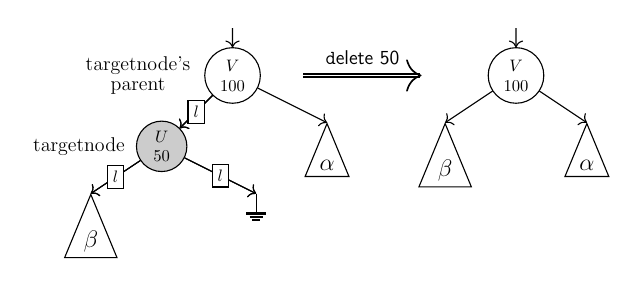
\begin{tikzpicture}[scale=0.6, transform shape,mylabel/.style={thin, draw=black, align=center, minimum width=0.3cm, minimum height=0.3cm,fill=white}]
		\newcommand\XA{-3}
		\newcommand\YA{0}
		\node (x)		[treenode] 																at (\XA,\YA)       					{$V$ \\ 100};
		\node (y)		[treenode, fill=black!20] 								at (\XA-1.5,\YA-1.5) 				{$U$ \\ 50};
		\node (a)		[subtree] 																at (\XA+2,\YA-1)      			{\Large $\alpha$};
		\node (b)		[subtree] 																at (\XA-3,\YA-2.5)    			{\Large $\beta$};
		\node (gnd)	[ground] 																	at (\XA+0.5,\YA-2.5)				{}; 
		\node (xl) 	[rectangle,align=center,minimum size=1cm] at (\XA-2,\YA) 							{\large targetnode's \\ \large parent};
		\node (yl) 	[] 																				at (\XA-3.25,\YA-1.5) 			{\large targetnode};
		
 		\draw[->] (x) -- (y);
 		\draw[->] (y) -- (b.north);
 		\draw[->] (y) -- (gnd);
		\draw[->] (\XA,\YA+1) -- (x);
		\draw[->] (x) -- (a.north);
		\pause
		\draw[->] (x) -- node[mylabel] {$\boldsymbol{l}$} (y);
		\pause
		\draw[->] (y) -- node[mylabel] {$\boldsymbol{l}$} (b.north);
		\pause
		\draw[->] (y) -- node[mylabel] {$\boldsymbol{l}$} (gnd);
    \pause
		\path[every node/.style={font=\sffamily\small}]
		(\XA+1.5,\YA) edge[->,semithick, double] 							node [above, outer sep=3pt] {\large \texttt delete 50} (\XA+4,\YA);
		
		\node (ix)	[treenode] 																at (\XA+6,\YA) 							{$V$ \\ 100};
		\node (ib)	[subtree] 																at (\XA+4.5,\YA-1)					{\Large $\beta$};
		\node (ia)	[subtree] 																at (\XA+7.5,\YA-1) 					{\Large $\alpha$};

		\draw[->] (\XA+6,\YA+1) -- (ix);
		\draw[->] (ix) -- (ib.north);
		\draw[->] (ix) -- (ia.north);
	\end{tikzpicture}
\end{frame}

\begin{frame}[c]{Lock Based BST - Complex Delete}
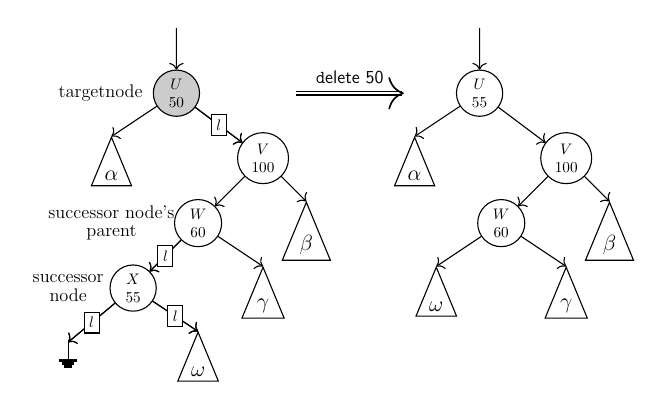
\begin{tikzpicture}[scale=0.55, transform shape,mylabel/.style={thin, draw=black, align=center, minimum width=0.3cm, minimum height=0.3cm,fill=white}]
		\newcommand\XA{0}
		\newcommand\YA{0}
		\node (x)		[treenode, fill=black!20] 	at (-6,0)       							{$U$ \\ 50};
		\node (a)		[subtree] 									at (-7.5,-1)  								{\Large $\alpha$};
		\node (y0)	[treenode] 									at (-4,-1.5) 									{$V$ \\ 100};
		\node (y1)	[treenode]									at (-5.5,-3)									{$W$ \\ 60}; 
		\node (b)		[subtree] 									at (-3,-2.5)    							{\Large $\beta$};
		\node (y2)	[treenode]									at (-7,-4.5)									{$X$ \\ 55}; 
		\node (g)		[subtree] 									at (-4,-4)   									{\Large $\gamma$};
		\node (gnd)	[ground] 										at (-8.5,-5.75)									{}; 
		\node (o)		[subtree] 									at (-5.5,-5.5)  							{\Large $\omega$};
		\node (x1) 	[] 													at (-7.75,0) 									{\large targetnode};
		\node (y1l) [rectangle,align=center,minimum size=1cm] at (-7.5,-3) 		{\large successor node's \\ \large parent};
		\node (y2l) [rectangle,align=center,minimum size=1cm] at(-8.5,-4.5) 	{\large successor \\ \large node};
		
		\draw[->] (-6, 1.5) --  (x);
		\draw[->] (x) -- (y0);
		\draw[->] (x) -- (a.north);
		\draw[->] (y0) -- (y1);
		\draw[->] (y0) -- (b.north);
		\draw[->] (y1) -- (y2);
		\draw[->] (y1) -- (g.north);
		\draw[->] (y2) -- (gnd);
		\draw[->] (y2) -- (o.north);
    \pause
    \draw[->] (x) -- node[mylabel] {$\boldsymbol{l}$} (y0);
    \pause
    \draw[->] (y1) -- node[mylabel] {$\boldsymbol{l}$} (y2);
    \pause
    \draw[->] (y2) -- node[mylabel] {$\boldsymbol{l}$} (gnd);
    \pause
  	\draw[->] (y2) -- node[mylabel] {$\boldsymbol{l}$} (o.north);
    \pause
		\path[every node/.style={font=\sffamily\small}]
		(-3.25, 0) edge[->,semithick, double] node [above, outer sep=3pt] 		{\large \texttt delete 50} (-0.75, 0);

		\node (ix)	[treenode] 									at (1,0)       								{$U$ \\ 55};
		\node (ia)	[subtree] 									at (-0.5,-1)  								{\Large $\alpha$};
		\node (iy0)	[treenode] 									at (3,-1.5) 									{$V$ \\ 100};
		\node (iy1)	[treenode]									at (1.5,-3)										{$W$ \\ 60}; 
		\node (ib)	[subtree] 									at (4,-2.5)    								{\Large $\beta$};
		\node (io)	[subtree]										at (0,-4)											{\Large $\omega$}; 
		\node (ignd)[subtree] 									at (3,-4)   									{\Large $\gamma$};
    
    \draw[->] (1, 1.5) --  (ix);
    \draw[->] (ix) --  (iy0);
    \draw[->] (ix) --  (ia.north);
    \draw[->] (iy0) --  (iy1);
    \draw[->] (iy0) --  (ib.north);
    \draw[->] (iy1) --  (io.north);
    \draw[->] (iy1) --  (ignd.north);
	\end{tikzpicture}
\end{frame}

\begin{frame}{Lock Based BST - More challenges in search}
A scenario in which the last right turn node is removed
\begin{figure}
\centering
{
	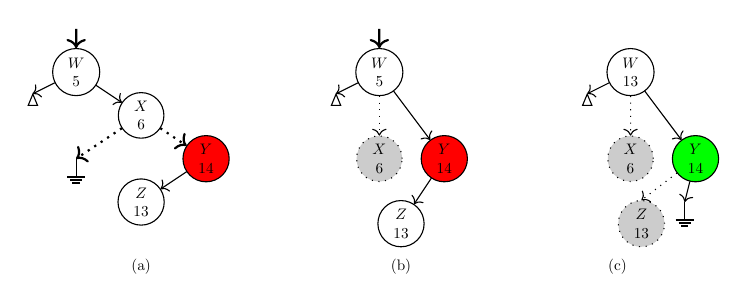
\begin{tikzpicture}[scale=0.55, transform shape]
		\newcommand\XA{-7}
		\newcommand\YA{0}
		\node[] at (-5.5,-4.5) {(a)};
		\node (x)		[treenode] 									at (\XA,\YA)       						{$W$ \\ 5};
		\node (S1)	[subtree,scale=0.5] 				at ([shift=({-1,-0.5})]x)  		{};
		\node (y0)	[treenode] 									at ([shift=({1.5,-1})]x) 			{$X$ \\ 6};
		\node (gnd)	[ground]										at ([shift=({-1.5,-1})]y0)		{}; 
		\node (y1)	[treenode,fill=red] 				at ([shift=({1.5,-1})]y0)   	{$Y$ \\ 14};
		\node (y2)	[treenode] 									at ([shift=({-1.5,-1})]y1)  	{$Z$ \\ 13};
		%\node (S2)	[subtree,scale=0.5]					at ([shift=({0.5,-1})]y1)			{}; 

		\path[every node/.style={font=\sffamily\large}]
		(\XA,\YA+1) 	edge[->,thick] 		node 					{} (x)
		(x) 		edge[->]								node 					{} (S1.north)
		(x) 		edge[->]								node 					{} (y0)
		(y0) 		edge[->,dotted,thick]		node 					{} (gnd)
		(y0) 		edge[->,dotted,thick]		node 					{} (y1)
		(y1) 		edge[->]								node 					{} (y2);
		%(y1) 		edge[->]							node 					{} (S2.north);
		\pause
		\renewcommand\XA{0}
		\node[] at (0.5,-4.5) {(b)};
		\node (ix)	[treenode] 										at (\XA,\YA)       						{$W$ \\ 5};
		\node (iS1)	[subtree,scale=0.5] 					at ([shift=({-1,-0.5})]ix)  	{};
		\node (iy1)	[treenode,fill=red] 					at ([shift=({1.5,-2})]ix)   {$Y$ \\ 14};
		\node (iy2)	[treenode] 										at ([shift=({-1,-1.5})]iy1)  	{$Z$ \\ 13};
		%\node (iS2)	[subtree,scale=0.5]					at ([shift=({0.5,-1.0})]iy1)	{}; 
		\node (iy0)	[treenode, fill=black!20, dotted] at ([shift=({0,-2})]ix) {$X$ \\ 6};

		\path[every node/.style={font=\sffamily\large}]
		(\XA,\YA+1) 	edge[->,thick] 		node 					{} (ix)
		(ix) 		edge[->]								node 					{} (iS1.north)
		(ix) 		edge[->]								node 					{} (iy1)
		(ix) 		edge[->,dotted]					node 					{} (iy0)
		(iy1) 	edge[->]								node 					{} (iy2);
		%(iy1) 	edge[->]								node 					{} (iS2.north);
		\pause
		\renewcommand\XA{5.8}
		\node[] at (5.5,-4.5) {(c)};
		\node (iix)		[treenode] 									at (\XA,\YA)       							{$W$ \\ 13};
		\node (iiS1)	[subtree,scale=0.5] 				at ([shift=({-1,-0.5})]iix)  		{};
		\node (iiy1)	[treenode,fill=green] 			at ([shift=({1.5,-2})]iix)  		{$Y$ \\ 14};
		\node (iignd)	[ground]										at ([shift=({-0.25,-1})]iiy1)				{}; 
		\node (iy0)	[treenode, fill=black!20, dotted] at ([shift=({0,-2})]iix) {$X$ \\ 6};
		\node (iy2)	[treenode, fill=black!20, dotted] at ([shift=({-1.25,-1.5})]iiy1){$Z$ \\ 13};
		
		\path[every node/.style={font=\sffamily\large}]
		(iix) 		edge[->]								node 					{} (iiS1.north)
		(iix) 		edge[->]								node 					{} (iiy1)
		(iix) 		edge[->,dotted]					node 					{} (iy0)
		(iiy1) 		edge[->,dotted]					node 					{} (iy2.north)
		(iiy1) 		edge[->]								node 					{} (iignd);	
	\end{tikzpicture}
}
\end{figure}

\begin{itemize}
\item<1> \footnotesize Search(13) gets stalled at $Y$ in (a). Its last right turn node is $X$
\item<2> \footnotesize Delete(6) removes $X$ from the tree in (b). The key stored in $X$ is still 6
\item<3> \footnotesize Delete(5) results in 13 moving up the tree from $Z$ to $W$ in (c). When search(13) wakes up, it will miss 13 as the key in the last right turn node has not changed
\end{itemize}


\begin{itemize}
\item<4> \footnotesize In the first traversal search(13) saw the node $X$
\item<4> \footnotesize In the second traversal there are two cases
\begin{itemize}
\item<4> \tiny case1, search(13) did not find $X$ - save the traversal and restart
\item<4> \tiny case2, search(13) did find $X$ - use the results of previous traversal
\end{itemize}
\end{itemize}

\end{frame}


\section{Lock Free Binary Search Tree}
\begin{frame}[c]{Lock Free BST[ICDCN'15]}
Contributions
\begin{itemize}
\item combine edge-based locking with internal representation of BST 
\item optimistic tree traversal 
\pause
\item lock-free algorithm
\end{itemize}
\end{frame}

\begin{frame}{Lock Free BST[ICDCN'15]}
\begin{itemize}
\item search and inserts are same as in lock Based BST
\item to maintain lock-free property, if an insert or delete operation fails, it helps a pending delete operation(if needed)
\end{itemize} 
%\ifdefined\LONG
pseudocode for delete
\begin{algorithm}[H]
locate the node to delete\;
flag the children edges for deletion\;
\uIf{simple delete}
{
make the parent point to the non-null child atomically\;
}
\Else(// complex delete)
{
find the successor\;
flag the children edges of successor for promotion\;
promote key\;
remove successor by a simple delete\;
replace node with a fresh copy\;
}
\end{algorithm}
%\fi
\end{frame}

\begin{frame}[c]{Lock Free BST - Simple Delete}
\begin{itemize}
\item flag is owned by an operation
\item if a thread which installed the flag is stalled, other threads can help complete the operation
\end{itemize}
\pause
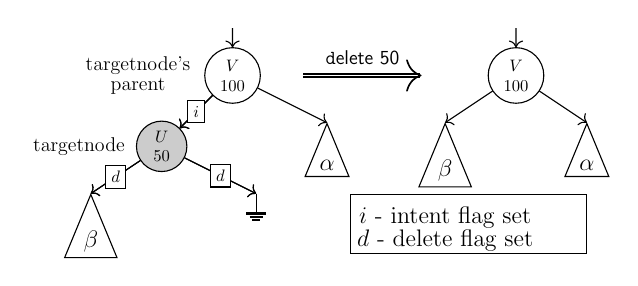
\begin{tikzpicture}[scale=0.6, transform shape,mylabel/.style={thin, draw=black, align=center, minimum width=0.3cm, minimum height=0.3cm,fill=white}]
		\newcommand\XA{-3}
		\newcommand\YA{0}
		\node (x)		[treenode] 																at (\XA,\YA)       					{$V$ \\ 100};
		\node (y)		[treenode, fill=black!20] 								at (\XA-1.5,\YA-1.5) 				{$U$ \\ 50};
		\node (a)		[subtree] 																at (\XA+2,\YA-1)      			{\Large $\alpha$};
		\node (b)		[subtree] 																at (\XA-3,\YA-2.5)    			{\Large $\beta$};
		\node (gnd)	[ground] 																	at (\XA+0.5,\YA-2.5)				{}; 
		\node (xl) 	[rectangle,align=center,minimum size=1cm] at (\XA-2,\YA) 							{\large targetnode's \\ \large parent};
		\node (yl) 	[] 																				at (\XA-3.25,\YA-1.5) 			{\large targetnode};
		
 		\draw[->] (x) -- (y);
 		\draw[->] (y) -- (b.north);
 		\draw[->] (y) -- (gnd);
		\draw[->] (\XA,\YA+1) -- (x);
		\draw[->] (x) -- (a.north);
		\pause
		%% legend
		\node (l1) 																						at (\XA+4.5,\YA-3){\Large $\boldsymbol{i}$  - \Large intent flag set};
		\node (l2) 																						at (\XA+4.5,\YA-3.5){\Large $\boldsymbol{d}$  - \Large delete flag set};
		\node [thin, draw=black, align=center, minimum width=5cm, minimum height=1.25cm] at (\XA+5,\YA-3.15) {};	
		\draw[->] (x) -- node[mylabel] {$\boldsymbol{i}$} (y);
		%\draw[->] (x) -- node[mylabel] {$\boldsymbol{f}$} (y);
		\pause
		\draw[->] (y) -- node[mylabel] {$\boldsymbol{d}$} (b.north);
		%\draw[->] (y) -- node[mylabel] {$\boldsymbol{f}$} (b.north);
		\pause
		\draw[->] (y) -- node[mylabel] {$\boldsymbol{d}$} (gnd);
		%\draw[->] (y) -- node[mylabel] {$\boldsymbol{f}$} (gnd);
    \pause
		\path[every node/.style={font=\sffamily\small}]
		(\XA+1.5,\YA) edge[->,semithick, double] 							node [above, outer sep=3pt] {\large \texttt delete 50} (\XA+4,\YA);
		
		\node (ix)	[treenode] 																at (\XA+6,\YA) 							{$V$ \\ 100};
		\node (ib)	[subtree] 																at (\XA+4.5,\YA-1)					{\Large $\beta$};
		\node (ia)	[subtree] 																at (\XA+7.5,\YA-1) 					{\Large $\alpha$};

		\draw[->] (\XA+6,\YA+1) -- (ix);
		\draw[->] (ix) -- (ib.north);
		\draw[->] (ix) -- (ia.north);
	\end{tikzpicture}
\end{frame}

\begin{frame}[c]{Lock Free BST - Complex Delete}
\input{figures/ICDCNcomplexDelete1}
\end{frame}
\begin{frame}[c]{Lock Free BST - Complex Delete}
\input{figures/ICDCNcomplexDelete2}
\end{frame}

\section{Local recovery}
%\begin{limitscope}
%%%%% local recovery experiments macros - begin
\newcommand{\retries}{\emph {retries}}
\newcommand{\seekTime}{\emph {seek-time}}
\newcommand{\modifyTime}{\emph {modify-time}}
\newcommand{\seekLength}{\emph {seek-length}}
\newcommand{\estLatencyImpact}{\emph {latency-impact}}
\newcommand{\throughput}{\emph {throughput}}
\newcommand{\action}{modify}
%%%%% local recovery experiments macros - end

In this section we evaluate our local recovery technique. 

To show that our local recovery algorithm is sufficiently general, we implemented it for three different concurrent internal BSTs, namely those based on:
\begin{enumerate*}[label=(\roman*)]
\item the lock-free BST by Howley and Jones~\cite{HowJon:2012:SPAA}, denoted by \HJBST{},
\item the lock-based BST by Ramachandran and Mittal~\cite{RamMit:2015:PPoPP}, denoted by \CASTLE{} and
\item the RCU (Read-Copy-Update) lock-based BST by Arbel and Attiya~\cite{ArbAtt:2014:PODC}, denoted by \CITRUS{}.
\end{enumerate*}
These implementations were chosen so that we covered both lock-free and lock-based approaches. We choose two lock-based implementations as one is based on locking edges~\cite{RamMit:2015:PPoPP} and the other is based on locking nodes using RCU framework~\cite{ArbAtt:2014:PODC}.

\subsection*{Experimental Setup}
As local recovery is useful for high contention cases, we conducted our experiments on a single Intel Xeon Phi SE10P Coprocessor \footnote{http://www.intel.com/content/www/us/en/processors/xeon/xeon-phi-detail.html}
having 61 1.1 GHz cores with 4 hardware threads per core and 8GB of GDDR5 memory. With this machine we were able to experiment with up to 244 threads.

\subsection*{Key distribution}
Usually uniform key distribution (where all keys have same frequency of occurrence) have been used to evaluate concurrent BSTs. But in many of the real world workloads, keys have skewed distribution~\cite{ClaSha+:2009:SIAM} where some keys are more popular than others. Zipfian distribution, a type of power-law distribution simulates this behaviour~\cite{BreCao+:1999:INFOCOM,FalJag:1992:VLDB,GraSun+:1994:SIGMOD}. It is characterized by a parameter $\alpha$ which usually lies between 0.5 and 1~\cite{BreCao+:1999:INFOCOM,AdaHub:2002:GLOTTMET}. In our experiments we used both uniform and Zipfian distributions to evaluate the local recovery algorithm.

\subsection*{Simulation results}
\Tabref{localRecovery-perf-numbers} summarizes the performance gap (with respect to system throughput) between the base algorithm and its extension using local recovery for uniform and Zipfian distributions. 
\begin{table}[tp]
\centering
\caption{Effect of local recovery on system throughput. Positive number indicates a gain while a negative number indicates a drop.}
\label{tab:perf-numbers}
\begin{tabular}{|c|c|c|}
\hline
{\bf Algorithm}  & {\bf \begin{tabular}[c]{@{}c@{}}Uniform\\ (max\%, min\%)\end{tabular}} & {\bf \begin{tabular}[c]{@{}c@{}}Zipfian\\ (max\%, min\%)\end{tabular}} \\ \hline
{\bf \CASTLE{}} & (6, -7)                                                            & (23, -11)                                                            \\ \hline
{\bf \CITRUS{}} & (23, -11)                                                            & (20, -13)                                                             \\ \hline
{\bf \HJBST{}}  & (9, -6)                                                            & (49, -6)                                                           \\ \hline
\end{tabular}
\end{table}

To better understand the effect of local recovery, we also measure several metrics defined in \tabref{metrics-definition}.
\begin{table}
\centering
\caption{Performance metrics used to evaluate the effect of local recovery.}
\label{tab:metrics-definition}
\begin{tabular}{|l|>{}m{0.7\linewidth}|}
\hline
{\bf Metric}					& {\bf Description} 		\\ \hline
{\retries} 				& { fraction of restarts for an operation}      					\\ \hline
{\seekTime}  					& {total time an operation spends on tree traversal including all restarts as well as stack processing time (in $\mu$s)}  \\ \hline
{\modifyTime}  					& {total time an operation spends on \action{} phase (in $\mu$s)}      					\\ \hline
{\seekLength} 				& {number of nodes traversed in the tree by an operation}      					\\ \hline
{\estLatencyImpact}		& {a rough approximation of the amount of clock cycles devoted to each L1 cache miss (a measure of cache performance)~\cite{JefRei:2013:Book}}      					\\ \hline
\end{tabular}                
\end{table}
\Figsref{localRecovery-throughput-uniform}{metrics-uniform} show the impact of local recovery on throughput and various metrics for uniform distribution. We see that the performance gain is marginal and, in many cases, is actually slightly worse due to the overhead of stack maintenance. This is not surprising because, for small trees, even though contention is higher, seek time is small to begin with and any benefit of local recovery is nullified by additional overhead of stack maintenance. For larger trees, even though seek time is larger, contention is low as key accesses are spread evenly.
% Style to select only points from #1 to #2 (inclusive)
\pgfplotsset
{
	select coords between index/.style 2 args=
	{
    x filter/.code=
		{
        \ifnum\coordindex<#1\def\pgfmathresult{}\fi
        \ifnum\coordindex>#2\def\pgfmathresult{}\fi
    }
	}
}
\begin{figure}
\centering
\nextwithlateexternal% < added
\begin{tikzpicture}
	\begin{groupplot}[group style={group size= 4 by 3},height=5.25cm,width=4.5cm,max space between ticks=20,minor tick num=1,tick label style={font=\scriptsize}]
		\nextgroupplot[title={\scriptsize 2K keys},ylabel={\scriptsize Read-Dominated},y label style={at={(0.15,0.5)}},xtick={1,61,122,183,244},mark size=1.5pt]
				\addplot[black, densely dashed,mark=square] [select coords between index={0}{8}] 		table[x=NumOfThreads,y=citrus-MOPS,col sep=space]	 	{Data/localRecovery/mic/threadSweep-uniform.csv}; 	\label{plots:CITRUS:mopsU}
				\addplot[red,densely dashed,mark=triangle*] [select coords between index={0}{8}] 		table[x=NumOfThreads,y=howley-MOPS,col sep=space]	 	{Data/localRecovery/mic/threadSweep-uniform.csv}; 	\label{plots:HOWLEY:mopsU}
				%\addplot[blue,densely dashed,mark=asterisk][select coords between index={0}{8}] 		table[x=NumOfThreads,y=icdcn-MOPS,col sep=space] 	 	{Data/localRecovery/mic/threadSweep-uniform.csv};  	\label{plots:ICDCN:mopsU}
				\addplot[green, densely dashed,mark=o] 		 	[select coords between index={0}{8}] 		table[x=NumOfThreads,y=castle-MOPS,col sep=space]	 	{Data/localRecovery/mic/threadSweep-uniform.csv}; 	\label{plots:CASTLE:mopsU}
				\addplot[black, semithick,mark=square] 	  	[select coords between index={0}{8}] 		table[x=NumOfThreads,y=citrusL-MOPS,col sep=space]	{Data/localRecovery/mic/threadSweep-uniform.csv}; 	\label{plots:CITRUSL:mopsU}
				\addplot[red,semithick,mark=triangle*] 			[select coords between index={0}{8}] 		table[x=NumOfThreads,y=howleyL-MOPS,col sep=space]	{Data/localRecovery/mic/threadSweep-uniform.csv}; 	\label{plots:HOWLEYL:mopsU}
				%\addplot[blue,semithick,mark=asterisk] 		[select coords between index={0}{8}] 		table[x=NumOfThreads,y=icdcnL-MOPS,col sep=space] 	{Data/localRecovery/mic/threadSweep-uniform.csv};  	\label{plots:ICDCNL:mopsU}
				\addplot[green, semithick,mark=o] 					[select coords between index={0}{8}] 		table[x=NumOfThreads,y=castleL-MOPS,col sep=space]	{Data/localRecovery/mic/threadSweep-uniform.csv}; 	\label{plots:CASTLEL:mopsU}
				\coordinate (top) at (rel axis cs:0,1);% coordinate at top of the first plot	
		\nextgroupplot[title={\scriptsize 20K keys},xtick={1,61,122,183,244},mark size=1.5pt]	
				\addplot[black, densely dashed,mark=square] [select coords between index={9}{17}] 	table[x=NumOfThreads,y=citrus-MOPS,col sep=space] 	{Data/localRecovery/mic/threadSweep-uniform.csv};  
				\addplot[red,densely dashed,mark=triangle*] [select coords between index={9}{17}] 	table[x=NumOfThreads,y=howley-MOPS,col sep=space] 	{Data/localRecovery/mic/threadSweep-uniform.csv};  
				%\addplot[blue,densely dashed,mark=asterisk][select coords between index={9}{17}] 	table[x=NumOfThreads,y=icdcn-MOPS,col sep=space]  	{Data/localRecovery/mic/threadSweep-uniform.csv};  
				\addplot[green, densely dashed,mark=o] 			[select coords between index={9}{17}] 	table[x=NumOfThreads,y=castle-MOPS,col sep=space] 	{Data/localRecovery/mic/threadSweep-uniform.csv}; 
				\addplot[black, semithick,mark=square] 			[select coords between index={9}{17}] 	table[x=NumOfThreads,y=citrusL-MOPS,col sep=space] 	{Data/localRecovery/mic/threadSweep-uniform.csv};
				\addplot[red,semithick,mark=triangle*] 			[select coords between index={9}{17}] 	table[x=NumOfThreads,y=howleyL-MOPS,col sep=space] 	{Data/localRecovery/mic/threadSweep-uniform.csv};
				%\addplot[blue,semithick,mark=asterisk] 		[select coords between index={9}{17}] 	table[x=NumOfThreads,y=icdcnL-MOPS,col sep=space]  	{Data/localRecovery/mic/threadSweep-uniform.csv}; 
				\addplot[green, semithick,mark=o] 					[select coords between index={9}{17}] 	table[x=NumOfThreads,y=castleL-MOPS,col sep=space] 	{Data/localRecovery/mic/threadSweep-uniform.csv};
		\nextgroupplot[title={\scriptsize 200K keys},xtick={1,61,122,183,244},mark size=1.5pt]
				\addplot[black, densely dashed,mark=square] [select coords between index={18}{26}] 	table[x=NumOfThreads,y=citrus-MOPS,col sep=space] 	{Data/localRecovery/mic/threadSweep-uniform.csv};
				\addplot[red,densely dashed,mark=triangle*] [select coords between index={18}{26}] 	table[x=NumOfThreads,y=howley-MOPS,col sep=space] 	{Data/localRecovery/mic/threadSweep-uniform.csv};
				%\addplot[blue,densely dashed,mark=asterisk][select coords between index={18}{26}] 	table[x=NumOfThreads,y=icdcn-MOPS,col sep=space]  	{Data/localRecovery/mic/threadSweep-uniform.csv};
				\addplot[green, densely dashed,mark=o] 			[select coords between index={18}{26}] 	table[x=NumOfThreads,y=castle-MOPS,col sep=space] 	{Data/localRecovery/mic/threadSweep-uniform.csv};
				\addplot[black, semithick,mark=square] 			[select coords between index={18}{26}] 	table[x=NumOfThreads,y=citrusL-MOPS,col sep=space] 	{Data/localRecovery/mic/threadSweep-uniform.csv};
				\addplot[red,semithick,mark=triangle*] 			[select coords between index={18}{26}] 	table[x=NumOfThreads,y=howleyL-MOPS,col sep=space] 	{Data/localRecovery/mic/threadSweep-uniform.csv};
				%\addplot[blue,semithick,mark=asterisk] 		[select coords between index={18}{26}] 	table[x=NumOfThreads,y=icdcnL-MOPS,col sep=space]  	{Data/localRecovery/mic/threadSweep-uniform.csv}; 
				\addplot[green, semithick,mark=o] 					[select coords between index={18}{26}] 	table[x=NumOfThreads,y=castleL-MOPS,col sep=space] 	{Data/localRecovery/mic/threadSweep-uniform.csv};
		\nextgroupplot[title={\scriptsize 2M keys},xtick={1,61,122,183,244},mark size=1.5pt]	
				\addplot[black, densely dashed,mark=square] [select coords between index={27}{35}] 	table[x=NumOfThreads,y=citrus-MOPS,col sep=space] 	{Data/localRecovery/mic/threadSweep-uniform.csv}; 
				\addplot[red,densely dashed,mark=triangle*] [select coords between index={27}{35}] 	table[x=NumOfThreads,y=howley-MOPS,col sep=space] 	{Data/localRecovery/mic/threadSweep-uniform.csv};
				%\addplot[blue,densely dashed,mark=asterisk][select coords between index={27}{35}] 	table[x=NumOfThreads,y=icdcn-MOPS,col sep=space]  	{Data/localRecovery/mic/threadSweep-uniform.csv};
				\addplot[green, densely dashed,mark=o] 			[select coords between index={27}{35}] 	table[x=NumOfThreads,y=castle-MOPS,col sep=space] 	{Data/localRecovery/mic/threadSweep-uniform.csv};
				\addplot[black, semithick,mark=square] 			[select coords between index={27}{35}] 	table[x=NumOfThreads,y=citrusL-MOPS,col sep=space] 	{Data/localRecovery/mic/threadSweep-uniform.csv};
				\addplot[red,semithick,mark=triangle*] 			[select coords between index={27}{35}] 	table[x=NumOfThreads,y=howleyL-MOPS,col sep=space] 	{Data/localRecovery/mic/threadSweep-uniform.csv};
				%\addplot[blue,semithick,mark=asterisk] 		[select coords between index={27}{35}] 	table[x=NumOfThreads,y=icdcnL-MOPS,col sep=space]  	{Data/localRecovery/mic/threadSweep-uniform.csv}; 
				\addplot[green, semithick,mark=o] 					[select coords between index={27}{35}] 	table[x=NumOfThreads,y=castleL-MOPS,col sep=space] 	{Data/localRecovery/mic/threadSweep-uniform.csv};
		\nextgroupplot[ylabel={\scriptsize Mixed},y label style={at={(0.15,0.5)}},xtick={1,61,122,183,244},mark size=1.5pt]		
				\addplot[black, densely dashed,mark=square] [select coords between index={36}{44}] 	table[x=NumOfThreads,y=citrus-MOPS,col sep=space] 	{Data/localRecovery/mic/threadSweep-uniform.csv}; 
				\addplot[red,densely dashed,mark=triangle*] [select coords between index={36}{44}] 	table[x=NumOfThreads,y=howley-MOPS,col sep=space] 	{Data/localRecovery/mic/threadSweep-uniform.csv};
				%\addplot[blue,densely dashed,mark=asterisk][select coords between index={36}{44}] 	table[x=NumOfThreads,y=icdcn-MOPS,col sep=space]  	{Data/localRecovery/mic/threadSweep-uniform.csv};
				\addplot[green, densely dashed,mark=o] 			[select coords between index={36}{44}] 	table[x=NumOfThreads,y=castle-MOPS,col sep=space] 	{Data/localRecovery/mic/threadSweep-uniform.csv};
				\addplot[black, semithick,mark=square] 			[select coords between index={36}{44}] 	table[x=NumOfThreads,y=citrusL-MOPS,col sep=space] 	{Data/localRecovery/mic/threadSweep-uniform.csv};
				\addplot[red,semithick,mark=triangle*] 			[select coords between index={36}{44}] 	table[x=NumOfThreads,y=howleyL-MOPS,col sep=space] 	{Data/localRecovery/mic/threadSweep-uniform.csv};
				%\addplot[blue,semithick,mark=asterisk] 		[select coords between index={36}{44}] 	table[x=NumOfThreads,y=icdcnL-MOPS,col sep=space]  	{Data/localRecovery/mic/threadSweep-uniform.csv}; 
				\addplot[green, semithick,mark=o] 					[select coords between index={36}{44}] 	table[x=NumOfThreads,y=castleL-MOPS,col sep=space] 	{Data/localRecovery/mic/threadSweep-uniform.csv};
		\nextgroupplot[xtick={1,61,122,183,244},mark size=1.5pt]		
				\addplot[black, densely dashed,mark=square] [select coords between index={45}{53}] 	table[x=NumOfThreads,y=citrus-MOPS,col sep=space] 	{Data/localRecovery/mic/threadSweep-uniform.csv}; 
				\addplot[red,densely dashed,mark=triangle*] [select coords between index={45}{53}] 	table[x=NumOfThreads,y=howley-MOPS,col sep=space] 	{Data/localRecovery/mic/threadSweep-uniform.csv};
				%\addplot[blue,densely dashed,mark=asterisk][select coords between index={45}{53}] 	table[x=NumOfThreads,y=icdcn-MOPS,col sep=space]  	{Data/localRecovery/mic/threadSweep-uniform.csv};
				\addplot[green, densely dashed,mark=o] 			[select coords between index={45}{53}] 	table[x=NumOfThreads,y=castle-MOPS,col sep=space] 	{Data/localRecovery/mic/threadSweep-uniform.csv};
				\addplot[black, semithick,mark=square] 			[select coords between index={45}{53}] 	table[x=NumOfThreads,y=citrusL-MOPS,col sep=space] 	{Data/localRecovery/mic/threadSweep-uniform.csv};
				\addplot[red,semithick,mark=triangle*] 			[select coords between index={45}{53}] 	table[x=NumOfThreads,y=howleyL-MOPS,col sep=space] 	{Data/localRecovery/mic/threadSweep-uniform.csv};
				%\addplot[blue,semithick,mark=asterisk] 		[select coords between index={45}{53}] 	table[x=NumOfThreads,y=icdcnL-MOPS,col sep=space]  	{Data/localRecovery/mic/threadSweep-uniform.csv}; 
				\addplot[green, semithick,mark=o] 					[select coords between index={45}{53}] 	table[x=NumOfThreads,y=castleL-MOPS,col sep=space] 	{Data/localRecovery/mic/threadSweep-uniform.csv};
		\nextgroupplot[xtick={1,61,122,183,244},mark size=1.5pt]		
				\addplot[black, densely dashed,mark=square] [select coords between index={54}{62}] 	table[x=NumOfThreads,y=citrus-MOPS,col sep=space] 	{Data/localRecovery/mic/threadSweep-uniform.csv}; 
				\addplot[red,densely dashed,mark=triangle*] [select coords between index={54}{62}] 	table[x=NumOfThreads,y=howley-MOPS,col sep=space] 	{Data/localRecovery/mic/threadSweep-uniform.csv};
				%\addplot[blue,densely dashed,mark=asterisk][select coords between index={54}{62}] 	table[x=NumOfThreads,y=icdcn-MOPS,col sep=space]  	{Data/localRecovery/mic/threadSweep-uniform.csv};
				\addplot[green, densely dashed,mark=o] 			[select coords between index={54}{62}] 	table[x=NumOfThreads,y=castle-MOPS,col sep=space] 	{Data/localRecovery/mic/threadSweep-uniform.csv};	
				\addplot[black, semithick,mark=square] 			[select coords between index={54}{62}] 	table[x=NumOfThreads,y=citrusL-MOPS,col sep=space] 	{Data/localRecovery/mic/threadSweep-uniform.csv};
				\addplot[red,semithick,mark=triangle*] 			[select coords between index={54}{62}] 	table[x=NumOfThreads,y=howleyL-MOPS,col sep=space] 	{Data/localRecovery/mic/threadSweep-uniform.csv};
				%\addplot[blue,semithick,mark=asterisk] 		[select coords between index={54}{62}] 	table[x=NumOfThreads,y=icdcnL-MOPS,col sep=space]  	{Data/localRecovery/mic/threadSweep-uniform.csv}; 
				\addplot[green, semithick,mark=o] 					[select coords between index={54}{62}] 	table[x=NumOfThreads,y=castleL-MOPS,col sep=space] 	{Data/localRecovery/mic/threadSweep-uniform.csv};
		\nextgroupplot[xtick={1,61,122,183,244},mark size=1.5pt]		
				\addplot[black, densely dashed,mark=square] [select coords between index={63}{71}] 	table[x=NumOfThreads,y=citrus-MOPS,col sep=space] 	{Data/localRecovery/mic/threadSweep-uniform.csv}; 
				\addplot[red,densely dashed,mark=triangle*] [select coords between index={63}{71}] 	table[x=NumOfThreads,y=howley-MOPS,col sep=space] 	{Data/localRecovery/mic/threadSweep-uniform.csv};
				%\addplot[blue,densely dashed,mark=asterisk][select coords between index={63}{71}] 	table[x=NumOfThreads,y=icdcn-MOPS,col sep=space]  	{Data/localRecovery/mic/threadSweep-uniform.csv};
				\addplot[green, densely dashed,mark=o] 			[select coords between index={63}{71}] 	table[x=NumOfThreads,y=castle-MOPS,col sep=space] 	{Data/localRecovery/mic/threadSweep-uniform.csv};
				\addplot[black, semithick,mark=square] 			[select coords between index={63}{71}] 	table[x=NumOfThreads,y=citrusL-MOPS,col sep=space] 	{Data/localRecovery/mic/threadSweep-uniform.csv};
				\addplot[red,semithick,mark=triangle*] 			[select coords between index={63}{71}] 	table[x=NumOfThreads,y=howleyL-MOPS,col sep=space] 	{Data/localRecovery/mic/threadSweep-uniform.csv};
				%\addplot[blue,semithick,mark=asterisk] 		[select coords between index={63}{71}] 	table[x=NumOfThreads,y=icdcnL-MOPS,col sep=space]  	{Data/localRecovery/mic/threadSweep-uniform.csv}; 
				\addplot[green, semithick,mark=o] 					[select coords between index={63}{71}] 	table[x=NumOfThreads,y=castleL-MOPS,col sep=space] 	{Data/localRecovery/mic/threadSweep-uniform.csv};				
		\nextgroupplot[xlabel={\scriptsize Number of Threads},ylabel={\scriptsize Write-Dominated},y label style={at={(0.15,0.5)}},xtick={1,61,122,183,	244},mark size=1.5pt]
				\addplot[black, densely dashed,mark=square] [select coords between index={72}{80}] 	table[x=NumOfThreads,y=citrus-MOPS,col sep=space] 	{Data/localRecovery/mic/threadSweep-uniform.csv};    
				\addplot[red,densely dashed,mark=triangle*] [select coords between index={72}{80}] 	table[x=NumOfThreads,y=howley-MOPS,col sep=space] 	{Data/localRecovery/mic/threadSweep-uniform.csv};    
				%\addplot[blue,densely dashed,mark=asterisk][select coords between index={72}{80}] 	table[x=NumOfThreads,y=icdcn-MOPS,col sep=space]  	{Data/localRecovery/mic/threadSweep-uniform.csv};     
				\addplot[green, densely dashed,mark=o] 			[select coords between index={72}{80}] 	table[x=NumOfThreads,y=castle-MOPS,col sep=space] 	{Data/localRecovery/mic/threadSweep-uniform.csv};	   
				\addplot[black, semithick,mark=square] 			[select coords between index={72}{80}] 	table[x=NumOfThreads,y=citrusL-MOPS,col sep=space] 	{Data/localRecovery/mic/threadSweep-uniform.csv}; 
				\addplot[red,semithick,mark=triangle*] 			[select coords between index={72}{80}] 	table[x=NumOfThreads,y=howleyL-MOPS,col sep=space] 	{Data/localRecovery/mic/threadSweep-uniform.csv};   
				%\addplot[blue,semithick,mark=asterisk] 		[select coords between index={72}{80}] 	table[x=NumOfThreads,y=icdcnL-MOPS,col sep=space]  	{Data/localRecovery/mic/threadSweep-uniform.csv};    
				\addplot[green, semithick,mark=o] 					[select coords between index={72}{80}] 	table[x=NumOfThreads,y=castleL-MOPS,col sep=space] 	{Data/localRecovery/mic/threadSweep-uniform.csv};	
		\nextgroupplot[xlabel={\scriptsize Number of Threads},xtick={1,61,122,183,244},mark size=1.5pt]	
				\addplot[black, densely dashed,mark=square] [select coords between index={81}{89}] 	table[x=NumOfThreads,y=citrus-MOPS,col sep=space] 	{Data/localRecovery/mic/threadSweep-uniform.csv}; 
				\addplot[red,densely dashed,mark=triangle*] [select coords between index={81}{89}] 	table[x=NumOfThreads,y=howley-MOPS,col sep=space] 	{Data/localRecovery/mic/threadSweep-uniform.csv};
				%\addplot[blue,densely dashed,mark=asterisk][select coords between index={81}{89}] 	table[x=NumOfThreads,y=icdcn-MOPS,col sep=space]  	{Data/localRecovery/mic/threadSweep-uniform.csv};
				\addplot[green, densely dashed,mark=o] 			[select coords between index={81}{89}] 	table[x=NumOfThreads,y=castle-MOPS,col sep=space] 	{Data/localRecovery/mic/threadSweep-uniform.csv};	
				\addplot[black, semithick,mark=square] 			[select coords between index={81}{89}] 	table[x=NumOfThreads,y=citrusL-MOPS,col sep=space] 	{Data/localRecovery/mic/threadSweep-uniform.csv};
				\addplot[red,semithick,mark=triangle*] 			[select coords between index={81}{89}] 	table[x=NumOfThreads,y=howleyL-MOPS,col sep=space] 	{Data/localRecovery/mic/threadSweep-uniform.csv};
				%\addplot[blue,semithick,mark=asterisk] 		[select coords between index={81}{89}] 	table[x=NumOfThreads,y=icdcnL-MOPS,col sep=space]  	{Data/localRecovery/mic/threadSweep-uniform.csv}; 
				\addplot[green, semithick,mark=o] 					[select coords between index={81}{89}] 	table[x=NumOfThreads,y=castleL-MOPS,col sep=space] 	{Data/localRecovery/mic/threadSweep-uniform.csv};
		\nextgroupplot[xlabel={\scriptsize Number of Threads},xtick={1,61,122,183,244},mark size=1.5pt]	
				\addplot[black, densely dashed,mark=square] [select coords between index={90}{98}] 	table[x=NumOfThreads,y=citrus-MOPS,col sep=space] 	{Data/localRecovery/mic/threadSweep-uniform.csv}; 
				\addplot[red,densely dashed,mark=triangle*] [select coords between index={90}{98}] 	table[x=NumOfThreads,y=howley-MOPS,col sep=space] 	{Data/localRecovery/mic/threadSweep-uniform.csv};
				%\addplot[blue,densely dashed,mark=asterisk][select coords between index={90}{98}] 	table[x=NumOfThreads,y=icdcn-MOPS,col sep=space]  	{Data/localRecovery/mic/threadSweep-uniform.csv};
				\addplot[green, densely dashed,mark=o] 			[select coords between index={90}{98}] 	table[x=NumOfThreads,y=castle-MOPS,col sep=space] 	{Data/localRecovery/mic/threadSweep-uniform.csv};	
				\addplot[black, semithick,mark=square] 			[select coords between index={90}{98}] 	table[x=NumOfThreads,y=citrusL-MOPS,col sep=space] 	{Data/localRecovery/mic/threadSweep-uniform.csv};
				\addplot[red,semithick,mark=triangle*] 			[select coords between index={90}{98}] 	table[x=NumOfThreads,y=howleyL-MOPS,col sep=space] 	{Data/localRecovery/mic/threadSweep-uniform.csv};
				%\addplot[blue,semithick,mark=asterisk] 		[select coords between index={90}{98}] 	table[x=NumOfThreads,y=icdcnL-MOPS,col sep=space]  	{Data/localRecovery/mic/threadSweep-uniform.csv}; 
				\addplot[green, semithick,mark=o] 					[select coords between index={90}{98}] 	table[x=NumOfThreads,y=castleL-MOPS,col sep=space] 	{Data/localRecovery/mic/threadSweep-uniform.csv};
		\nextgroupplot[xlabel={\scriptsize Number of Threads},xtick={1,61,122,183,244},mark size=1.5pt]	
				\addplot[black, densely dashed,mark=square] [select coords between index={99}{107}]	table[x=NumOfThreads,y=citrus-MOPS,col sep=space] 	{Data/localRecovery/mic/threadSweep-uniform.csv}; 
				\addplot[red,densely dashed,mark=triangle*] [select coords between index={99}{107}]	table[x=NumOfThreads,y=howley-MOPS,col sep=space] 	{Data/localRecovery/mic/threadSweep-uniform.csv};
				%\addplot[blue,densely dashed,mark=asterisk][select coords between index={99}{107}]	table[x=NumOfThreads,y=icdcn-MOPS,col sep=space]  	{Data/localRecovery/mic/threadSweep-uniform.csv};
				\addplot[green, densely dashed,mark=o] 			[select coords between index={99}{107}]	table[x=NumOfThreads,y=castle-MOPS,col sep=space] 	{Data/localRecovery/mic/threadSweep-uniform.csv};		
				\addplot[black, semithick,mark=square] 			[select coords between index={99}{107}]	table[x=NumOfThreads,y=citrusL-MOPS,col sep=space] 	{Data/localRecovery/mic/threadSweep-uniform.csv};
				\addplot[red,semithick,mark=triangle*] 			[select coords between index={99}{107}]	table[x=NumOfThreads,y=howleyL-MOPS,col sep=space] 	{Data/localRecovery/mic/threadSweep-uniform.csv};
				%\addplot[blue,semithick,mark=asterisk] 		[select coords between index={99}{107}]	table[x=NumOfThreads,y=icdcnL-MOPS,col sep=space]  	{Data/localRecovery/mic/threadSweep-uniform.csv}; 
				\addplot[green, semithick,mark=o] 					[select coords between index={99}{107}]	table[x=NumOfThreads,y=castleL-MOPS,col sep=space] 	{Data/localRecovery/mic/threadSweep-uniform.csv};				
				\coordinate (bot) at (rel axis cs:1,0);% coordinate at bottom of the last plot
\end{groupplot}
	\path (top-|current bounding box.west)-- node[anchor=south,rotate=90] {\scriptsize system throughput} (bot-|current bounding box.west);
	\path (top|-current bounding box.north)-- coordinate(legendpos) (bot|-current bounding box.north);
	\matrix[matrix of nodes, anchor=south, draw, inner sep=0.2em, draw] at ([yshift=1ex]legendpos)
  {
    \ref{plots:HOWLEY:mopsU}& 	\HJBST{} 				& [5pt]
    %\ref{plots:ICDCN:mopsU}& 	\ICDCN{} 				& [5pt]
    \ref{plots:CITRUS:mopsU}& 	\CITRUS{} 			& [5pt]
		\ref{plots:CASTLE:mopsU}& 	\CASTLE{} 			\\
		\ref{plots:HOWLEYL:mopsU}& 	\HJBST{} (LR)		& [5pt]
    %\ref{plots:ICDCNL:mopsU}& 	\ICDCN{} (LR)		& [5pt]
    \ref{plots:CITRUSL:mopsU}& 	\CITRUS{} (LR)	& [5pt]
		\ref{plots:CASTLEL:mopsU}& 	\CASTLE{}	(LR)	\\
	};
\end{tikzpicture}
\caption[Impact of local recovery on throughput - uniform distribution]{Comparison of throughput of different concurrent BST implementations with (solid lines) and without (dotted lines) local recovery for uniform distribution. Each row represents a workload type. Each column represents a key space range. Higher is better.}
\label{fig:localRecovery-throughput-uniform}
\end{figure}
% Style to select only points from #1 to #2 (inclusive)
\pgfplotsset{
  select row/.style={
    x filter/.code={\ifnum\coordindex=#1\else\def\pgfmathresult{}\fi}
  },
}

\definecolor{colorbrewer1}{RGB}{166,206,227}
\definecolor{colorbrewer2}{RGB}{31,120,180}
\definecolor{colorbrewer3}{RGB}{178,223,138}
\definecolor{colorbrewer4}{RGB}{51,160,44}
\definecolor{colorbrewer5}{RGB}{251,154,153}
\definecolor{colorbrewer6}{RGB}{227,26,28}
\definecolor{colorbrewer7}{RGB}{253,191,111}
\definecolor{colorbrewer8}{RGB}{255,127,0}
\definecolor{colorbrewer9}{RGB}{202,178,214}
\definecolor{colorbrewer10}{RGB}{106,61,154}
\definecolor{colorbrewer11}{RGB}{222,179,155}
\definecolor{colorbrewer12}{RGB}{177,89,40}
			
\pgfplotscreateplotcyclelist{paired}{
{draw=colorbrewer1 ,pattern color=colorbrewer1 ,pattern=horizontal lines},
{draw=colorbrewer2 ,pattern color=colorbrewer2 ,pattern=horizontal lines},
{draw=colorbrewer3 ,pattern color=colorbrewer3 ,pattern=vertical lines},
{draw=colorbrewer4 ,pattern color=colorbrewer4 ,pattern=vertical lines},
{draw=colorbrewer5 ,pattern color=colorbrewer5 ,pattern=north east lines},
{draw=colorbrewer6 ,pattern color=colorbrewer6 ,pattern=north east lines},
{draw=colorbrewer7 ,pattern color=colorbrewer7 ,pattern=north west lines},
{draw=colorbrewer8 ,pattern color=colorbrewer8 ,pattern=north west lines},
{draw=colorbrewer9 ,pattern color=colorbrewer9 ,pattern=grid},
{draw=colorbrewer10,pattern color=colorbrewer10,pattern=grid},
{draw=colorbrewer11,pattern color=colorbrewer11,pattern=crosshatch},
{draw=colorbrewer12,pattern color=colorbrewer12,pattern=crosshatch}}
			
\def\twinplot#1#2{
  \pgfplotsforeachungrouped \row in {0,...,5}{
      \edef\justplotit{
        \noexpand\addplot+[bar shift=(-0.5)*\pgfplotbarwidth]
          table [x=metric, select row=\row, y=#1] {#2};}
      \justplotit
			\edef\justplotit{
        \noexpand\addplot+[bar shift=(0.5)*\pgfplotbarwidth]
          table [x=metric, select row=\row, y=#1L] {#2};}
      \justplotit
  }
}

\begin{figure}
\centering
\nextwithlateexternal% < added
\begin{tikzpicture}
\begin{groupplot}
	[
    group style={group size= 3 by 6,xticklabels at=edge bottom},
    height=3.5cm,
    width=5cm,
    ybar=1pt,
    tick label style={font=\scriptsize},
    x tick label style={rotate=45,anchor=east},
    symbolic x coords={retries,seek-time,modify-time,seek-length,throughput},
    ylabel style={align=center},
		cycle list name=paired,
    max space between ticks=15,
		ymin=0
  ]
	\pgfkeys{/pgf/bar width=5.5pt}
	
	\nextgroupplot[title=\CASTLE,ylabel={\scriptsize 2K}] \twinplot{castle}{Data/localRecovery/mic/scaled/uniform/2k-90-9-1.csv}
	%\nextgroupplot[title=\ICDCN] 						\twinplot{icdcn}{Data/localRecovery/mic/scaled/uniform/2k-90-9-1.csv}
	\nextgroupplot[title=\CITRUS] 						\twinplot{citrus}{Data/localRecovery/mic/scaled/uniform/2k-90-9-1.csv}
	\nextgroupplot[title=\HJBST] 							\twinplot{howley}{Data/localRecovery/mic/scaled/uniform/2k-90-9-1.csv}
	\coordinate (mtop0) at (rel axis cs:0,1);% coordinate at top of the first plot
		
	\nextgroupplot[ylabel={\scriptsize 200K}]							\twinplot{castle}{Data/localRecovery/mic/scaled/uniform/200k-90-9-1.csv}
	%\nextgroupplot														\twinplot{icdcn}{Data/localRecovery/mic/scaled/uniform/200k-90-9-1.csv}
	\nextgroupplot														\twinplot{citrus}{Data/localRecovery/mic/scaled/uniform/200k-90-9-1.csv}
	\nextgroupplot														\twinplot{howley}{Data/localRecovery/mic/scaled/uniform/200k-90-9-1.csv}
	\coordinate (mbot0) at (rel axis cs:1,0);% coordinate at bottom of the last plot
	
	\nextgroupplot[ylabel={\scriptsize 2K}] 							\twinplot{castle}{Data/localRecovery/mic/scaled/uniform/2k-70-20-10.csv}
	%\nextgroupplot														\twinplot{icdcn}{Data/localRecovery/mic/scaled/uniform/2k-70-20-10.csv}
	\nextgroupplot						  							\twinplot{citrus}{Data/localRecovery/mic/scaled/uniform/2k-70-20-10.csv}
	\nextgroupplot						  							\twinplot{howley}{Data/localRecovery/mic/scaled/uniform/2k-70-20-10.csv}
	\coordinate (mtop) at (rel axis cs:0,1);% coordinate at top of the first plot
		
	\nextgroupplot[ylabel={\scriptsize 200K}]							\twinplot{castle}{Data/localRecovery/mic/scaled/uniform/200k-70-20-10.csv}
	%\nextgroupplot														\twinplot{icdcn}{Data/localRecovery/mic/scaled/uniform/200k-70-20-10.csv}
	\nextgroupplot														\twinplot{citrus}{Data/localRecovery/mic/scaled/uniform/200k-70-20-10.csv}
	\nextgroupplot														\twinplot{howley}{Data/localRecovery/mic/scaled/uniform/200k-70-20-10.csv}
	\coordinate (mbot) at (rel axis cs:1,0);% coordinate at bottom of the last plot
	
	\nextgroupplot[ylabel={\scriptsize 2K}]								\twinplot{castle}{Data/localRecovery/mic/scaled/uniform/2k-0-50-50.csv}
	%\nextgroupplot														\twinplot{icdcn}{Data/localRecovery/mic/scaled/uniform/2k-0-50-50.csv}
	\nextgroupplot														\twinplot{citrus}{Data/localRecovery/mic/scaled/uniform/2k-0-50-50.csv}
	\nextgroupplot														\twinplot{howley}{Data/localRecovery/mic/scaled/uniform/2k-0-50-50.csv}
	\coordinate (wtop) at (rel axis cs:0,1);% coordinate at top of the first plot
	
	\nextgroupplot[ylabel={\scriptsize 200K}]							\twinplot{castle}{Data/localRecovery/mic/scaled/uniform/200k-0-50-50.csv}
	%\nextgroupplot														\twinplot{icdcn}{Data/localRecovery/mic/scaled/uniform/200k-0-50-50.csv}
	\nextgroupplot														\twinplot{citrus}{Data/localRecovery/mic/scaled/uniform/200k-0-50-50.csv}
	\nextgroupplot														\twinplot{howley}{Data/localRecovery/mic/scaled/uniform/200k-0-50-50.csv}
	\coordinate (wbot) at (rel axis cs:1,0);% coordinate at bottom of the last plot	
	
\end{groupplot}
\path (mtop0-|current bounding box.west)-- node[anchor=south,rotate=90,yshift=-0.9cm] {\scriptsize Read-Dominated} (mbot0-|current bounding box.west);
\path (mtop-|current bounding box.west)-- node[anchor=south,rotate=90,yshift=-0.9cm] {\scriptsize Mixed} (mbot-|current bounding box.west);
\path (wtop-|current bounding box.west)-- node[anchor=south,rotate=90,yshift=-0.9cm] {\scriptsize Write-Dominated} (wbot-|current bounding box.west);
\end{tikzpicture}
\caption[Impact of local recovery on various metrics - uniform distribution]{Impact of local recovery on various metrics for two key space ranges (2K and 200K) with uniform key distribution.
}
\label{fig:metrics-uniform}
\end{figure}

\Figsref{localRecovery-throughput-zipf}{metrics-zipf} show the impact of local recovery on throughput and various metrics for Zipfian distribution.  In general, Zipfian distribution causes more contention than uniform distribution. So even for small trees for which seek times are smaller, we still see performance gains for mixed and write-dominated workloads. As the graphs show,  we see a consistent increase in throughput (up to \localRecoveryMaximumgap{}) using local recovery as we move from low contention scenarios (read-dominated workload and large tree size)  to high contention scenarios (write-dominated workload and small tree size). Specifically, we see up to 70\% and 31\% improvements for \HJBST{} and \CASTLE{} respectively. Except \CITRUS{}, the other two implementations scale fairly well up to 244 threads.
% Style to select only points from #1 to #2 (inclusive)
\pgfplotsset
{
	select coords between index/.style 2 args=
	{
    x filter/.code=
		{
        \ifnum\coordindex<#1\def\pgfmathresult{}\fi
        \ifnum\coordindex>#2\def\pgfmathresult{}\fi
    }
	}
}
\begin{figure}
\centering
\nextwithlateexternal% < added
\begin{tikzpicture}
	\begin{groupplot}[group style={group size= 4 by 3},height=5.25cm,width=4.5cm,max space between ticks=20,minor tick num=1,tick label style={font=\scriptsize}]
		\nextgroupplot[title={\scriptsize 2K keys},ylabel={\scriptsize Read-Dominated},y label style={at={(0.15,0.5)}},xtick={1,61,122,183,244},mark size=1.5pt]
				\addplot[black, densely dashed,mark=square] [select coords between index={0}{8}] 		table[x=NumOfThreads,y=citrus-MOPS,col sep=space]	 	{Data/localRecovery/mic/threadSweep-zipf.csv}; 	\label{plots:CITRUS:mopsZ}
				\addplot[red,densely dashed,mark=triangle*] [select coords between index={0}{8}] 		table[x=NumOfThreads,y=howley-MOPS,col sep=space]	 	{Data/localRecovery/mic/threadSweep-zipf.csv}; 	\label{plots:HOWLEY:mopsZ}
				%\addplot[blue,densely dashed,mark=asterisk][select coords between index={0}{8}] 		table[x=NumOfThreads,y=icdcn-MOPS,col sep=space] 	 	{Data/localRecovery/mic/threadSweep-zipf.csv};  \label{plots:ICDCN:mopsZ}
				\addplot[green, densely dashed,mark=o] 		 	[select coords between index={0}{8}] 		table[x=NumOfThreads,y=castle-MOPS,col sep=space]	 	{Data/localRecovery/mic/threadSweep-zipf.csv}; 	\label{plots:CASTLE:mopsZ}
				\addplot[black, semithick,mark=square] 	  	[select coords between index={0}{8}] 		table[x=NumOfThreads,y=citrusL-MOPS,col sep=space]	{Data/localRecovery/mic/threadSweep-zipf.csv}; 	\label{plots:CITRUSL:mopsZ}
				\addplot[red,semithick,mark=triangle*] 			[select coords between index={0}{8}] 		table[x=NumOfThreads,y=howleyL-MOPS,col sep=space]	{Data/localRecovery/mic/threadSweep-zipf.csv}; 	\label{plots:HOWLEYL:mopsZ}
				%\addplot[blue,semithick,mark=asterisk] 		[select coords between index={0}{8}] 		table[x=NumOfThreads,y=icdcnL-MOPS,col sep=space] 	{Data/localRecovery/mic/threadSweep-zipf.csv};  \label{plots:ICDCNL:mopsZ}
				\addplot[green, semithick,mark=o] 					[select coords between index={0}{8}] 		table[x=NumOfThreads,y=castleL-MOPS,col sep=space]	{Data/localRecovery/mic/threadSweep-zipf.csv}; 	\label{plots:CASTLEL:mopsZ}
				\coordinate (top) at (rel axis cs:0,1);% coordinate at top of the first plot	
		\nextgroupplot[title={\scriptsize 20K keys},xtick={1,61,122,183,244},mark size=1.5pt]	
				\addplot[black, densely dashed,mark=square] [select coords between index={9}{17}] 	table[x=NumOfThreads,y=citrus-MOPS,col sep=space] 	{Data/localRecovery/mic/threadSweep-zipf.csv};  
				\addplot[red,densely dashed,mark=triangle*] [select coords between index={9}{17}] 	table[x=NumOfThreads,y=howley-MOPS,col sep=space] 	{Data/localRecovery/mic/threadSweep-zipf.csv};  
				%\addplot[blue,densely dashed,mark=asterisk][select coords between index={9}{17}] 	table[x=NumOfThreads,y=icdcn-MOPS,col sep=space]  	{Data/localRecovery/mic/threadSweep-zipf.csv};  
				\addplot[green, densely dashed,mark=o] 			[select coords between index={9}{17}] 	table[x=NumOfThreads,y=castle-MOPS,col sep=space] 	{Data/localRecovery/mic/threadSweep-zipf.csv}; 
				\addplot[black, semithick,mark=square] 			[select coords between index={9}{17}] 	table[x=NumOfThreads,y=citrusL-MOPS,col sep=space] 	{Data/localRecovery/mic/threadSweep-zipf.csv};
				\addplot[red,semithick,mark=triangle*] 			[select coords between index={9}{17}] 	table[x=NumOfThreads,y=howleyL-MOPS,col sep=space] 	{Data/localRecovery/mic/threadSweep-zipf.csv};
				%\addplot[blue,semithick,mark=asterisk] 		[select coords between index={9}{17}] 	table[x=NumOfThreads,y=icdcnL-MOPS,col sep=space]  	{Data/localRecovery/mic/threadSweep-zipf.csv}; 
				\addplot[green, semithick,mark=o] 					[select coords between index={9}{17}] 	table[x=NumOfThreads,y=castleL-MOPS,col sep=space] 	{Data/localRecovery/mic/threadSweep-zipf.csv};
		\nextgroupplot[title={\scriptsize 200K keys},xtick={1,61,122,183,244},mark size=1.5pt]
				\addplot[black, densely dashed,mark=square] [select coords between index={18}{26}] 	table[x=NumOfThreads,y=citrus-MOPS,col sep=space] 	{Data/localRecovery/mic/threadSweep-zipf.csv};
				\addplot[red,densely dashed,mark=triangle*] [select coords between index={18}{26}] 	table[x=NumOfThreads,y=howley-MOPS,col sep=space] 	{Data/localRecovery/mic/threadSweep-zipf.csv};
				%\addplot[blue,densely dashed,mark=asterisk][select coords between index={18}{26}] 	table[x=NumOfThreads,y=icdcn-MOPS,col sep=space]  	{Data/localRecovery/mic/threadSweep-zipf.csv};
				\addplot[green, densely dashed,mark=o] 			[select coords between index={18}{26}] 	table[x=NumOfThreads,y=castle-MOPS,col sep=space] 	{Data/localRecovery/mic/threadSweep-zipf.csv};
				\addplot[black, semithick,mark=square] 			[select coords between index={18}{26}] 	table[x=NumOfThreads,y=citrusL-MOPS,col sep=space] 	{Data/localRecovery/mic/threadSweep-zipf.csv};
				\addplot[red,semithick,mark=triangle*] 			[select coords between index={18}{26}] 	table[x=NumOfThreads,y=howleyL-MOPS,col sep=space] 	{Data/localRecovery/mic/threadSweep-zipf.csv};
				%\addplot[blue,semithick,mark=asterisk] 		[select coords between index={18}{26}] 	table[x=NumOfThreads,y=icdcnL-MOPS,col sep=space]  	{Data/localRecovery/mic/threadSweep-zipf.csv}; 
				\addplot[green, semithick,mark=o] 					[select coords between index={18}{26}] 	table[x=NumOfThreads,y=castleL-MOPS,col sep=space] 	{Data/localRecovery/mic/threadSweep-zipf.csv};
		\nextgroupplot[title={\scriptsize 2M keys},xtick={1,61,122,183,244},mark size=1.5pt]	
				\addplot[black, densely dashed,mark=square] [select coords between index={27}{35}] 	table[x=NumOfThreads,y=citrus-MOPS,col sep=space] 	{Data/localRecovery/mic/threadSweep-zipf.csv}; 
				\addplot[red,densely dashed,mark=triangle*] [select coords between index={27}{35}] 	table[x=NumOfThreads,y=howley-MOPS,col sep=space] 	{Data/localRecovery/mic/threadSweep-zipf.csv};
				%\addplot[blue,densely dashed,mark=asterisk][select coords between index={27}{35}] 	table[x=NumOfThreads,y=icdcn-MOPS,col sep=space]  	{Data/localRecovery/mic/threadSweep-zipf.csv};
				\addplot[green, densely dashed,mark=o] 			[select coords between index={27}{35}] 	table[x=NumOfThreads,y=castle-MOPS,col sep=space] 	{Data/localRecovery/mic/threadSweep-zipf.csv};
				\addplot[black, semithick,mark=square] 			[select coords between index={27}{35}] 	table[x=NumOfThreads,y=citrusL-MOPS,col sep=space] 	{Data/localRecovery/mic/threadSweep-zipf.csv};
				\addplot[red,semithick,mark=triangle*] 			[select coords between index={27}{35}] 	table[x=NumOfThreads,y=howleyL-MOPS,col sep=space] 	{Data/localRecovery/mic/threadSweep-zipf.csv};
				%\addplot[blue,semithick,mark=asterisk] 		[select coords between index={27}{35}] 	table[x=NumOfThreads,y=icdcnL-MOPS,col sep=space]  	{Data/localRecovery/mic/threadSweep-zipf.csv}; 
				\addplot[green, semithick,mark=o] 					[select coords between index={27}{35}] 	table[x=NumOfThreads,y=castleL-MOPS,col sep=space] 	{Data/localRecovery/mic/threadSweep-zipf.csv};
		\nextgroupplot[ylabel={\scriptsize Mixed},y label style={at={(0.15,0.5)}},xtick={1,61,122,183,244},mark size=1.5pt]		
				\addplot[black, densely dashed,mark=square] [select coords between index={36}{44}] 	table[x=NumOfThreads,y=citrus-MOPS,col sep=space] 	{Data/localRecovery/mic/threadSweep-zipf.csv}; 
				\addplot[red,densely dashed,mark=triangle*] [select coords between index={36}{44}] 	table[x=NumOfThreads,y=howley-MOPS,col sep=space] 	{Data/localRecovery/mic/threadSweep-zipf.csv};
				%\addplot[blue,densely dashed,mark=asterisk][select coords between index={36}{44}] 	table[x=NumOfThreads,y=icdcn-MOPS,col sep=space]  	{Data/localRecovery/mic/threadSweep-zipf.csv};
				\addplot[green, densely dashed,mark=o] 			[select coords between index={36}{44}] 	table[x=NumOfThreads,y=castle-MOPS,col sep=space] 	{Data/localRecovery/mic/threadSweep-zipf.csv};
				\addplot[black, semithick,mark=square] 			[select coords between index={36}{44}] 	table[x=NumOfThreads,y=citrusL-MOPS,col sep=space] 	{Data/localRecovery/mic/threadSweep-zipf.csv};
				\addplot[red,semithick,mark=triangle*] 			[select coords between index={36}{44}] 	table[x=NumOfThreads,y=howleyL-MOPS,col sep=space] 	{Data/localRecovery/mic/threadSweep-zipf.csv};
				%\addplot[blue,semithick,mark=asterisk] 		[select coords between index={36}{44}] 	table[x=NumOfThreads,y=icdcnL-MOPS,col sep=space]  	{Data/localRecovery/mic/threadSweep-zipf.csv}; 
				\addplot[green, semithick,mark=o] 					[select coords between index={36}{44}] 	table[x=NumOfThreads,y=castleL-MOPS,col sep=space] 	{Data/localRecovery/mic/threadSweep-zipf.csv};
		\nextgroupplot[xtick={1,61,122,183,244},mark size=1.5pt]		
				\addplot[black, densely dashed,mark=square] [select coords between index={45}{53}] 	table[x=NumOfThreads,y=citrus-MOPS,col sep=space] 	{Data/localRecovery/mic/threadSweep-zipf.csv}; 
				\addplot[red,densely dashed,mark=triangle*] [select coords between index={45}{53}] 	table[x=NumOfThreads,y=howley-MOPS,col sep=space] 	{Data/localRecovery/mic/threadSweep-zipf.csv};
				%\addplot[blue,densely dashed,mark=asterisk][select coords between index={45}{53}] 	table[x=NumOfThreads,y=icdcn-MOPS,col sep=space]  	{Data/localRecovery/mic/threadSweep-zipf.csv};
				\addplot[green, densely dashed,mark=o] 			[select coords between index={45}{53}] 	table[x=NumOfThreads,y=castle-MOPS,col sep=space] 	{Data/localRecovery/mic/threadSweep-zipf.csv};
				\addplot[black, semithick,mark=square] 			[select coords between index={45}{53}] 	table[x=NumOfThreads,y=citrusL-MOPS,col sep=space] 	{Data/localRecovery/mic/threadSweep-zipf.csv};
				\addplot[red,semithick,mark=triangle*] 			[select coords between index={45}{53}] 	table[x=NumOfThreads,y=howleyL-MOPS,col sep=space] 	{Data/localRecovery/mic/threadSweep-zipf.csv};
				%\addplot[blue,semithick,mark=asterisk] 		[select coords between index={45}{53}] 	table[x=NumOfThreads,y=icdcnL-MOPS,col sep=space]  	{Data/localRecovery/mic/threadSweep-zipf.csv}; 
				\addplot[green, semithick,mark=o] 					[select coords between index={45}{53}] 	table[x=NumOfThreads,y=castleL-MOPS,col sep=space] 	{Data/localRecovery/mic/threadSweep-zipf.csv};
		\nextgroupplot[xtick={1,61,122,183,244},mark size=1.5pt]		
				\addplot[black, densely dashed,mark=square] [select coords between index={54}{62}] 	table[x=NumOfThreads,y=citrus-MOPS,col sep=space] 	{Data/localRecovery/mic/threadSweep-zipf.csv}; 
				\addplot[red,densely dashed,mark=triangle*] [select coords between index={54}{62}] 	table[x=NumOfThreads,y=howley-MOPS,col sep=space] 	{Data/localRecovery/mic/threadSweep-zipf.csv};
				%\addplot[blue,densely dashed,mark=asterisk][select coords between index={54}{62}] 	table[x=NumOfThreads,y=icdcn-MOPS,col sep=space]  	{Data/localRecovery/mic/threadSweep-zipf.csv};
				\addplot[green, densely dashed,mark=o] 			[select coords between index={54}{62}] 	table[x=NumOfThreads,y=castle-MOPS,col sep=space] 	{Data/localRecovery/mic/threadSweep-zipf.csv};	
				\addplot[black, semithick,mark=square] 			[select coords between index={54}{62}] 	table[x=NumOfThreads,y=citrusL-MOPS,col sep=space] 	{Data/localRecovery/mic/threadSweep-zipf.csv};
				\addplot[red,semithick,mark=triangle*] 			[select coords between index={54}{62}] 	table[x=NumOfThreads,y=howleyL-MOPS,col sep=space] 	{Data/localRecovery/mic/threadSweep-zipf.csv};
				%\addplot[blue,semithick,mark=asterisk] 		[select coords between index={54}{62}] 	table[x=NumOfThreads,y=icdcnL-MOPS,col sep=space]  	{Data/localRecovery/mic/threadSweep-zipf.csv}; 
				\addplot[green, semithick,mark=o] 					[select coords between index={54}{62}] 	table[x=NumOfThreads,y=castleL-MOPS,col sep=space] 	{Data/localRecovery/mic/threadSweep-zipf.csv};
		\nextgroupplot[xtick={1,61,122,183,244},mark size=1.5pt]		
				\addplot[black, densely dashed,mark=square] [select coords between index={63}{71}] 	table[x=NumOfThreads,y=citrus-MOPS,col sep=space] 	{Data/localRecovery/mic/threadSweep-zipf.csv}; 
				\addplot[red,densely dashed,mark=triangle*] [select coords between index={63}{71}] 	table[x=NumOfThreads,y=howley-MOPS,col sep=space] 	{Data/localRecovery/mic/threadSweep-zipf.csv};
				%\addplot[blue,densely dashed,mark=asterisk][select coords between index={63}{71}] 	table[x=NumOfThreads,y=icdcn-MOPS,col sep=space]  	{Data/localRecovery/mic/threadSweep-zipf.csv};
				\addplot[green, densely dashed,mark=o] 			[select coords between index={63}{71}] 	table[x=NumOfThreads,y=castle-MOPS,col sep=space] 	{Data/localRecovery/mic/threadSweep-zipf.csv};
				\addplot[black, semithick,mark=square] 			[select coords between index={63}{71}] 	table[x=NumOfThreads,y=citrusL-MOPS,col sep=space] 	{Data/localRecovery/mic/threadSweep-zipf.csv};
				\addplot[red,semithick,mark=triangle*] 			[select coords between index={63}{71}] 	table[x=NumOfThreads,y=howleyL-MOPS,col sep=space] 	{Data/localRecovery/mic/threadSweep-zipf.csv};
				%\addplot[blue,semithick,mark=asterisk] 		[select coords between index={63}{71}] 	table[x=NumOfThreads,y=icdcnL-MOPS,col sep=space]  	{Data/localRecovery/mic/threadSweep-zipf.csv}; 
				\addplot[green, semithick,mark=o] 					[select coords between index={63}{71}] 	table[x=NumOfThreads,y=castleL-MOPS,col sep=space] 	{Data/localRecovery/mic/threadSweep-zipf.csv};				
		\nextgroupplot[xlabel={\scriptsize Number of Threads},ylabel={\scriptsize Write-Dominated},y label style={at={(0.15,0.5)}},xtick={1,61,122,183,	244},mark size=1.5pt]
				\addplot[black, densely dashed,mark=square] [select coords between index={72}{80}] 	table[x=NumOfThreads,y=citrus-MOPS,col sep=space] 	{Data/localRecovery/mic/threadSweep-zipf.csv};    
				\addplot[red,densely dashed,mark=triangle*] [select coords between index={72}{80}] 	table[x=NumOfThreads,y=howley-MOPS,col sep=space] 	{Data/localRecovery/mic/threadSweep-zipf.csv};    
				%\addplot[blue,densely dashed,mark=asterisk][select coords between index={72}{80}] 	table[x=NumOfThreads,y=icdcn-MOPS,col sep=space]  	{Data/localRecovery/mic/threadSweep-zipf.csv};     
				\addplot[green, densely dashed,mark=o] 			[select coords between index={72}{80}] 	table[x=NumOfThreads,y=castle-MOPS,col sep=space] 	{Data/localRecovery/mic/threadSweep-zipf.csv};	   
				\addplot[black, semithick,mark=square] 			[select coords between index={72}{80}] 	table[x=NumOfThreads,y=citrusL-MOPS,col sep=space] 	{Data/localRecovery/mic/threadSweep-zipf.csv}; 
				\addplot[red,semithick,mark=triangle*] 			[select coords between index={72}{80}] 	table[x=NumOfThreads,y=howleyL-MOPS,col sep=space] 	{Data/localRecovery/mic/threadSweep-zipf.csv};   
				%\addplot[blue,semithick,mark=asterisk] 		[select coords between index={72}{80}] 	table[x=NumOfThreads,y=icdcnL-MOPS,col sep=space]  	{Data/localRecovery/mic/threadSweep-zipf.csv};    
				\addplot[green, semithick,mark=o] 					[select coords between index={72}{80}] 	table[x=NumOfThreads,y=castleL-MOPS,col sep=space] 	{Data/localRecovery/mic/threadSweep-zipf.csv};	
		\nextgroupplot[xlabel={\scriptsize Number of Threads},xtick={1,61,122,183,244},mark size=1.5pt]	
				\addplot[black, densely dashed,mark=square] [select coords between index={81}{89}] 	table[x=NumOfThreads,y=citrus-MOPS,col sep=space] 	{Data/localRecovery/mic/threadSweep-zipf.csv}; 
				\addplot[red,densely dashed,mark=triangle*] [select coords between index={81}{89}] 	table[x=NumOfThreads,y=howley-MOPS,col sep=space] 	{Data/localRecovery/mic/threadSweep-zipf.csv};
				%\addplot[blue,densely dashed,mark=asterisk][select coords between index={81}{89}] 	table[x=NumOfThreads,y=icdcn-MOPS,col sep=space]  	{Data/localRecovery/mic/threadSweep-zipf.csv};
				\addplot[green, densely dashed,mark=o] 			[select coords between index={81}{89}] 	table[x=NumOfThreads,y=castle-MOPS,col sep=space] 	{Data/localRecovery/mic/threadSweep-zipf.csv};	
				\addplot[black, semithick,mark=square] 			[select coords between index={81}{89}] 	table[x=NumOfThreads,y=citrusL-MOPS,col sep=space] 	{Data/localRecovery/mic/threadSweep-zipf.csv};
				\addplot[red,semithick,mark=triangle*] 			[select coords between index={81}{89}] 	table[x=NumOfThreads,y=howleyL-MOPS,col sep=space] 	{Data/localRecovery/mic/threadSweep-zipf.csv};
				%\addplot[blue,semithick,mark=asterisk] 		[select coords between index={81}{89}] 	table[x=NumOfThreads,y=icdcnL-MOPS,col sep=space]  	{Data/localRecovery/mic/threadSweep-zipf.csv}; 
				\addplot[green, semithick,mark=o] 					[select coords between index={81}{89}] 	table[x=NumOfThreads,y=castleL-MOPS,col sep=space] 	{Data/localRecovery/mic/threadSweep-zipf.csv};
		\nextgroupplot[xlabel={\scriptsize Number of Threads},xtick={1,61,122,183,244},mark size=1.5pt]	
				\addplot[black, densely dashed,mark=square] [select coords between index={90}{98}] 	table[x=NumOfThreads,y=citrus-MOPS,col sep=space] 	{Data/localRecovery/mic/threadSweep-zipf.csv}; 
				\addplot[red,densely dashed,mark=triangle*] [select coords between index={90}{98}] 	table[x=NumOfThreads,y=howley-MOPS,col sep=space] 	{Data/localRecovery/mic/threadSweep-zipf.csv};
				%\addplot[blue,densely dashed,mark=asterisk][select coords between index={90}{98}] 	table[x=NumOfThreads,y=icdcn-MOPS,col sep=space]  	{Data/localRecovery/mic/threadSweep-zipf.csv};
				\addplot[green, densely dashed,mark=o] 			[select coords between index={90}{98}] 	table[x=NumOfThreads,y=castle-MOPS,col sep=space] 	{Data/localRecovery/mic/threadSweep-zipf.csv};	
				\addplot[black, semithick,mark=square] 			[select coords between index={90}{98}] 	table[x=NumOfThreads,y=citrusL-MOPS,col sep=space] 	{Data/localRecovery/mic/threadSweep-zipf.csv};
				\addplot[red,semithick,mark=triangle*] 			[select coords between index={90}{98}] 	table[x=NumOfThreads,y=howleyL-MOPS,col sep=space] 	{Data/localRecovery/mic/threadSweep-zipf.csv};
				%\addplot[blue,semithick,mark=asterisk] 		[select coords between index={90}{98}] 	table[x=NumOfThreads,y=icdcnL-MOPS,col sep=space]  	{Data/localRecovery/mic/threadSweep-zipf.csv}; 
				\addplot[green, semithick,mark=o] 					[select coords between index={90}{98}] 	table[x=NumOfThreads,y=castleL-MOPS,col sep=space] 	{Data/localRecovery/mic/threadSweep-zipf.csv};
		\nextgroupplot[xlabel={\scriptsize Number of Threads},xtick={1,61,122,183,244},mark size=1.5pt]	
				\addplot[black, densely dashed,mark=square] [select coords between index={99}{107}]	table[x=NumOfThreads,y=citrus-MOPS,col sep=space] 	{Data/localRecovery/mic/threadSweep-zipf.csv}; 
				\addplot[red,densely dashed,mark=triangle*] [select coords between index={99}{107}]	table[x=NumOfThreads,y=howley-MOPS,col sep=space] 	{Data/localRecovery/mic/threadSweep-zipf.csv};
				%\addplot[blue,densely dashed,mark=asterisk][select coords between index={99}{107}]	table[x=NumOfThreads,y=icdcn-MOPS,col sep=space]  	{Data/localRecovery/mic/threadSweep-zipf.csv};
				\addplot[green, densely dashed,mark=o] 			[select coords between index={99}{107}]	table[x=NumOfThreads,y=castle-MOPS,col sep=space] 	{Data/localRecovery/mic/threadSweep-zipf.csv};		
				\addplot[black, semithick,mark=square] 			[select coords between index={99}{107}]	table[x=NumOfThreads,y=citrusL-MOPS,col sep=space] 	{Data/localRecovery/mic/threadSweep-zipf.csv};
				\addplot[red,semithick,mark=triangle*] 			[select coords between index={99}{107}]	table[x=NumOfThreads,y=howleyL-MOPS,col sep=space] 	{Data/localRecovery/mic/threadSweep-zipf.csv};
				%\addplot[blue,semithick,mark=asterisk] 		[select coords between index={99}{107}]	table[x=NumOfThreads,y=icdcnL-MOPS,col sep=space]  	{Data/localRecovery/mic/threadSweep-zipf.csv}; 
				\addplot[green, semithick,mark=o] 					[select coords between index={99}{107}]	table[x=NumOfThreads,y=castleL-MOPS,col sep=space] 	{Data/localRecovery/mic/threadSweep-zipf.csv};				
				\coordinate (bot) at (rel axis cs:1,0);% coordinate at bottom of the last plot
\end{groupplot}
	\path (top-|current bounding box.west)-- node[anchor=south,rotate=90] {\scriptsize system throughput} (bot-|current bounding box.west);
	\path (top|-current bounding box.north)-- coordinate(legendpos) (bot|-current bounding box.north);
	\matrix[matrix of nodes, anchor=south, draw, inner sep=0.2em, draw] at ([yshift=1ex]legendpos)
  {
    \ref{plots:HOWLEY:mopsZ}&  \HJBST{} 				& [5pt]
    %\ref{plots:ICDCN:mopsZ}&  \ICDCN{} 				& [5pt]
    \ref{plots:CITRUS:mopsZ}&  \CITRUS{} 				& [5pt]
		\ref{plots:CASTLE:mopsZ}&  \CASTLE{} 				\\
		\ref{plots:HOWLEYL:mopsZ}& \HJBST{} (LR)		& [5pt]
    %\ref{plots:ICDCNL:mopsZ}& \ICDCN{} (LR)		& [5pt]
    \ref{plots:CITRUSL:mopsZ}& \CITRUS{} (LR)	& [5pt]
		\ref{plots:CASTLEL:mopsZ}& \CASTLE{}	(LR)	\\
	};
\end{tikzpicture}
\caption[Impact of local recovery on throughput - zipf distribution]{Comparison of throughput of different concurrent BST implementations with (solid lines) and without (dotted lines) local recovery for zipfian distribution with $\alpha$=1. Each row represents a workload type. Each column represents a key space range. Higher is better.}
\label{fig:localRecovery-throughput-zipf}
\end{figure}
\input{experiments/localRecovery/experiments-graphs-mic-localRecovery-metrics-coloured-zipf}

As shown in \Figref{metrics-zipf}, for \HJBST{}, all the metrics except \modifyTime{} show improvement.
A modify operation in this algorithm helps any pending operation along its traversal path leading to higher fraction of restarts shown by the metric \retries.
Retries and hence \seekLength{} and \seekTime{} are significantly reduced due to local recovery.

For \CASTLE{}, for smaller trees, we see that all the metrics improved and the throughput increases up to 31\%.
For \CITRUS{}, there was no improvement due to local recovery across all three workloads as this algorithm is optimized for low contention scenarios and does not scale well for high contention scenarios.
Most of its modify operation's time is spent on \action{} phase than in seek phase.
The main reason being a complex delete operation has to wait till all previous readers have completed their traversals.

\begin{comment}
From \figsrefc[ and ]{localRecovery-throughput-stampede-threadSweep-zipf-4Set-Relative}{localRecovery-seekTime-stampede-threadSweep-zipf-4Set-Relative}, we see a clear correlation between seek time and system throughput. As seek time reduces due to local recovery, the system throughput also improves. We see maximum improvement for \HJBST{}. Since \CASTLE{} and \CITRUS{} are lock-based algorithms, no helping is performed during tree traversal.  But in \HJBST{}, during the tree traversal, if a pending operation is seen it is helped and then the current operation is restarted. This results in frequent restarts and hence local recovery improves performance by a larger margin.
\end{comment}
%\end{limitscope}

\section{Experimental Evaluation}
We now describe the results of the comparative evaluation of different implementations of a concurrent BST using simulated workloads. This chapter is organized as follows. Performance evaluation of our lock-based algorithm is described in \secref{experiments:castle} followed by our lock-free algorithm described in \secref{experiments:icdcn}. Performance evaluation of our local recovery technique is described in \secref{experiments:localRecovery}.

\section{Experimental Setup} 
We conducted our experiments on a single large-memory node in stampede\footnote{https://www.tacc.utexas.edu/systems/stampede} cluster at TACC (Texas Advanced Computing Center). This node is a Dell PowerEdge R820 server with 4 Intel E5-4650 8-core processors (32 cores in total) and 1TB of DDR3 memory. Hyper-threading has been disabled on the node. It runs CentOS 6.3 operating system.  

To better understand the scalability of our algorithms we also conducted experiments on a single Intel Xeon Phi SE10P Coprocessor\footnote{http://www.intel.com/content/www/us/en/processors/xeon/xeon-phi-detail.html} having 61 1.1 GHz cores with 4 hardware threads per core and 8GB of GDDR5 memory.

We used Intel C/C++ compiler (version 2013.2.146) with optimization flag set to O3. We used GNU Scientific Library to generate random numbers. We used Intel's \emph{TBB Malloc}~\cite{Rei:2007:Book} as the dynamic memory allocator since it provided superior performance to C/C+ default allocator in a multi-threaded environment.

To compare the performance of different implementations, we considered the following parameters:
\begin{enumerate}[leftmargin=*, noitemsep]
\item \textbf{Relative Distribution of Operations:} We considered three different workload  distributions: 
						\begin{enumerate*}[label=(\alph*)]
						\item \emph{read-dominated:} 90\% search, 9\% insert and 1\% delete, 
						\item \emph{mixed:} 70\% search, 20\% insert and 10\% delete, and
						\item \emph{write-dominated:} 0\% search, 50\% insert and 50\% delete.
						\end{enumerate*}
\item \textbf{Maximum Degree of Contention:} This depends on number of threads that can concurrently operate on the tree. On 32 core machine, we varied the number of threads 
from 1 to 32 in powers of two. On 61 core machine we varied the number of threads from 1 to 244 in multiples of 61.
\item \textbf{Maximum Tree Size:} This depends on the size of the key space. To get the peak throughput, we set the number of threads to be the value where the peak performance is achieved and we varied key space size from 2\textsuperscript{13} (8Ki) to 2\textsuperscript{24} (16Mi).  To understand the scalability of the algorithms, we varied the number of threads and considered three different key ranges: 20,000 (20K), 200,000 (200K) and 2 million (2M) keys.
\end{enumerate}

We compared the performance of different algorithms with respect to \emph{system throughput}, given by the number of operations executed per unit time. In each run of the experiment, we ran each algorithm for 2 minutes, and calculated the total number of operations completed by the end of the run to determine the system throughput. The results were averaged over 5 runs. To capture only the steady state behaviour, we \textit{pre-populated} the tree to 50\% of its maximum size, prior to starting a simulation run. The beginning of each run consisted of a 1 second ``warm-up'' phase whose numbers were excluded in the computed statistics to avoid initial caching effects. 

\section{Lock based tree}
\label{sec:experiments:castle}
In this section we evaluate \CASTLE{} against three other implementations of a concurrent 
BST, namely those based on:
%%
\begin{enumerate}[label=(\roman*)]
\item the lock-free internal BST by Howley and Jones~\cite{HowJon:2012:SPAA}, denoted by \HJBST{},
\item the lock-free external BST by Natarajan and Mittal~\cite{NatMit:2014:PPoPP}, denoted by \NMBST{}, and 
\item the RCU-based internal BST by Arbel and Attiya~\cite{ArbAtt:2014:PODC}, denoted by \CITRUS{}.
\end{enumerate}
%%
Note that \CITRUS{} is a blocking implementation. The above three implementations were obtained from their respective authors. All implementations were written in C/C++. In our experiments, none of the implementations used garbage collection to reclaim memory. The experimental evaluation in~\cite{HowJon:2012:SPAA, NatMit:2014:PPoPP} showed that, in all cases,  either \HJBST{} or \NMBST{} outperformed the concurrent BST implementation based on Ellen \emph{et al.}'s lock-free algorithm in~\cite{EllFat+:2010:PODC}. So we did not consider it in our experiments. 
\input{c06/castle/graphs-castle-stampede-threadSweep}
% Style to select only points from #1 to #2 (inclusive)
\pgfplotsset
{
	select coords between index/.style 2 args=
	{
    x filter/.code=
		{
        \ifnum\coordindex<#1\def\pgfmathresult{}\fi
        \ifnum\coordindex>#2\def\pgfmathresult{}\fi
    }
	}
}
\begin{figure}[htp]
\centering
\begin{tikzpicture}[scale=0.9, transform shape]
	\begin{groupplot}[group style={group size= 3 by 3},height=3cm,width=4cm,xmode=log,log basis x={2},max space between ticks=20,minor tick num=1,tick label style={font=\tiny},xlabel style={font=\tiny},ylabel style={font=\tiny}, title style={font=\tiny}]
		\nextgroupplot[title=Small,ylabel={Read-Dominated},xtick=data]
				\addplot[brown, semithick,mark=square,mark size=1] 	[select coords between index={0}{3}] table[x=keyspace,y=Mops-citrus,col sep=space]{Data/snb32/keySweep.csv};  \label{plots:CITRUS:cka}
				\addplot[red,semithick,mark=triangle,mark size=1] 	[select coords between index={0}{3}] table[x=keyspace,y=Mops-howley,col sep=space]{Data/snb32/keySweep.csv};  \label{plots:HJ-BST:cka}
				\addplot[blue,semithick,mark=asterisk,mark size=1] 	[select coords between index={0}{3}] table[x=keyspace,y=Mops-ppop,col sep=space]{Data/snb32/keySweep.csv};  	\label{plots:NM-BST:cka}
				\addplot[green, semithick,mark=o,mark size=1] 			[select coords between index={0}{3}] table[x=keyspace,y=Mops-castle,col sep=space]{Data/snb32/keySweep.csv};  \label{plots:RM-LOCK:cka}
				\coordinate (top) at (rel axis cs:0,1);% coordinate at top of the first plot
		\nextgroupplot[title=Medium,xtick=data]
				\addplot[brown, semithick,mark=square,mark size=1] 	[select coords between index={4}{7}] table[x=keyspace,y=Mops-citrus,col sep=space]{Data/snb32/keySweep.csv}; 
				\addplot[red,semithick,mark=triangle,mark size=1] 	[select coords between index={4}{7}] table[x=keyspace,y=Mops-howley,col sep=space]{Data/snb32/keySweep.csv}; 
				\addplot[blue,semithick,mark=asterisk,mark size=1] 	[select coords between index={4}{7}] table[x=keyspace,y=Mops-ppop,col sep=space]{Data/snb32/keySweep.csv};   
				\addplot[green, semithick,mark=o,mark size=1] 			[select coords between index={4}{7}] table[x=keyspace,y=Mops-castle,col sep=space]{Data/snb32/keySweep.csv};
		\nextgroupplot[title=Large,xtick=data]
				\addplot[brown, semithick,mark=square,mark size=1] 	[select coords between index={8}{11}] table[x=keyspace,y=Mops-citrus,col sep=space]{Data/snb32/keySweep.csv};
				\addplot[red,semithick,mark=triangle,mark size=1] 	[select coords between index={8}{11}] table[x=keyspace,y=Mops-howley,col sep=space]{Data/snb32/keySweep.csv};
				\addplot[blue,semithick,mark=asterisk,mark size=1] 	[select coords between index={8}{11}] table[x=keyspace,y=Mops-ppop,col sep=space]{Data/snb32/keySweep.csv};  
				\addplot[green, semithick,mark=o,mark size=1] 			[select coords between index={8}{11}] table[x=keyspace,y=Mops-castle,col sep=space]{Data/snb32/keySweep.csv};
		\nextgroupplot[ylabel={Mixed},xtick=data]
				\addplot[brown, semithick,mark=square,mark size=1] 	[select coords between index={12}{15}] table[x=keyspace,y=Mops-citrus,col sep=space]{Data/snb32/keySweep.csv};
				\addplot[red,semithick,mark=triangle,mark size=1] 	[select coords between index={12}{15}] table[x=keyspace,y=Mops-howley,col sep=space]{Data/snb32/keySweep.csv};
				\addplot[blue,semithick,mark=asterisk,mark size=1] 	[select coords between index={12}{15}] table[x=keyspace,y=Mops-ppop,col sep=space]{Data/snb32/keySweep.csv};  
				\addplot[green, semithick,mark=o,mark size=1] 			[select coords between index={12}{15}] table[x=keyspace,y=Mops-castle,col sep=space]{Data/snb32/keySweep.csv};
		\nextgroupplot[xtick=data]
				\addplot[brown, semithick,mark=square,mark size=1] 	[select coords between index={16}{19}] table[x=keyspace,y=Mops-citrus,col sep=space]{Data/snb32/keySweep.csv};
				\addplot[red,semithick,mark=triangle,mark size=1] 	[select coords between index={16}{19}] table[x=keyspace,y=Mops-howley,col sep=space]{Data/snb32/keySweep.csv};
				\addplot[blue,semithick,mark=asterisk,mark size=1] 	[select coords between index={16}{19}] table[x=keyspace,y=Mops-ppop,col sep=space]{Data/snb32/keySweep.csv};  
				\addplot[green, semithick,mark=o,mark size=1] 			[select coords between index={16}{19}] table[x=keyspace,y=Mops-castle,col sep=space]{Data/snb32/keySweep.csv};
		\nextgroupplot[xtick=data]
				\addplot[brown, semithick,mark=square,mark size=1] 	[select coords between index={20}{23}] table[x=keyspace,y=Mops-citrus,col sep=space]{Data/snb32/keySweep.csv};
				\addplot[red,semithick,mark=triangle,mark size=1] 	[select coords between index={20}{23}] table[x=keyspace,y=Mops-howley,col sep=space]{Data/snb32/keySweep.csv};
				\addplot[blue,semithick,mark=asterisk,mark size=1] 	[select coords between index={20}{23}] table[x=keyspace,y=Mops-ppop,col sep=space]{Data/snb32/keySweep.csv};  
				\addplot[green, semithick,mark=o,mark size=1] 			[select coords between index={20}{23}] table[x=keyspace,y=Mops-castle,col sep=space]{Data/snb32/keySweep.csv};
		\nextgroupplot[xlabel={Key Space Size},ylabel={Write-Dominated},xtick=data]
				\addplot[brown, semithick,mark=square,mark size=1] 	[select coords between index={24}{27}] table[x=keyspace,y=Mops-citrus,col sep=space]{Data/snb32/keySweep.csv}; 
				\addplot[red,semithick,mark=triangle,mark size=1] 	[select coords between index={24}{27}] table[x=keyspace,y=Mops-howley,col sep=space]{Data/snb32/keySweep.csv};
				\addplot[blue,semithick,mark=asterisk,mark size=1] 	[select coords between index={24}{27}] table[x=keyspace,y=Mops-ppop,col sep=space]{Data/snb32/keySweep.csv};  
				\addplot[green, semithick,mark=o,mark size=1] 			[select coords between index={24}{27}] table[x=keyspace,y=Mops-castle,col sep=space]{Data/snb32/keySweep.csv};	
		\nextgroupplot[xlabel={Key Space Size},xtick=data]
				\addplot[brown, semithick,mark=square,mark size=1] 	[select coords between index={28}{31}] table[x=keyspace,y=Mops-citrus,col sep=space]{Data/snb32/keySweep.csv};
				\addplot[red,semithick,mark=triangle,mark size=1] 	[select coords between index={28}{31}] table[x=keyspace,y=Mops-howley,col sep=space]{Data/snb32/keySweep.csv};
				\addplot[blue,semithick,mark=asterisk,mark size=1] 	[select coords between index={28}{31}] table[x=keyspace,y=Mops-ppop,col sep=space]{Data/snb32/keySweep.csv};  
				\addplot[green, semithick,mark=o,mark size=1] 			[select coords between index={28}{31}] table[x=keyspace,y=Mops-castle,col sep=space]{Data/snb32/keySweep.csv};
		\nextgroupplot[xlabel={Key Space Size},xtick=data]
				\addplot[brown, semithick,mark=square,mark size=1] 	[select coords between index={32}{35}] table[x=keyspace,y=Mops-citrus,col sep=space]{Data/snb32/keySweep.csv}; 
				\addplot[red,semithick,mark=triangle,mark size=1] 	[select coords between index={32}{35}] table[x=keyspace,y=Mops-howley,col sep=space]{Data/snb32/keySweep.csv};
				\addplot[blue,semithick,mark=asterisk,mark size=1] 	[select coords between index={32}{35}] table[x=keyspace,y=Mops-ppop,col sep=space]{Data/snb32/keySweep.csv};  
				\addplot[green, semithick,mark=o,mark size=1] 			[select coords between index={32}{35}] table[x=keyspace,y=Mops-castle,col sep=space]{Data/snb32/keySweep.csv};						
				\coordinate (bot) at (rel axis cs:1,0);% coordinate at bottom of the last plot
	\end{groupplot}
	\path (top-|current bounding box.west)-- node[anchor=south,rotate=90] {\tiny System throughput (million operations/second)} (bot-|current bounding box.west);
	\path (top|-current bounding box.north)-- coordinate(legendpos) (bot|-current bounding box.north);
	\matrix[matrix of nodes, anchor=south, draw, inner sep=0.2em, draw] at ([yshift=1ex]legendpos)
  {
    \ref{plots:HJ-BST:cka}& \tiny \HJBST{} & [5pt]
    \ref{plots:NM-BST:cka}& \tiny \NMBST{} & [5pt]
    \ref{plots:CITRUS:cka}& \tiny \CITRUS{} & [5pt]
		\ref{plots:RM-LOCK:cka}& \tiny \CASTLE{} \\
	};
\end{tikzpicture}
%\caption[\CASTLE{} - Comparison of throughput of different algorithms - key sweep]{Comparison of system throughput of different algorithms at 32 threads. Each row represents a workload type. Each column represents a range of key space range. Higher the ratio, better the performance of the algorithm.}
\label{fig:castle-keySweep-absolute}
\end{figure}

The results of our experiments are shown in  \figref{castle-threadSweep} and \figref{castle-keySweep-absolute}. In \figref{castle-threadSweep}, the absolute value of the system throughput is plotted against the number of threads (varying from 1 to 32 in powers of 2). Here each row represents a specific workload (read-dominated, mixed or write-dominated) and each column represents a specific key space size (20K, 200K and 2M). In \figref{castle-keySweep-absolute}, the value of the system throughput is plotted against the key space size. Here each column represents a range of key space sizes (small, medium and large) and each row represents a specific workload. As the peak performance for all the four algorithms (for all cases) occurred at 32 threads, we set the number of threads to 32 while varying the key space size from $2^{13}$ to $2^{24}$.

As both \figref{castle-threadSweep} and \figref{castle-keySweep-absolute} show, for smaller key space sizes, \NMBST{} achieves the best system throughput. This is not surprising since \NMBST{} is optimized for high contention scenarios. For medium and large key space sizes, \CASTLE{} achieves the best system throughput for all three workload types in almost all the cases (except when the workload is write-dominated and the key space size is in the lower half of the medium range). The maximum gap between \CASTLE{} and the next best performer is around \castleMaximumgap{} which occurs at 500K key space size, read-dominated workload and 32 threads.

We believe that some of the reasons for the better performance of  \CASTLE{} over the other three concurrent algorithms, especially when the contention is relatively low,  are as follows. First, as explained in~\cite{NatMit:2014:PPoPP}, operating at edge-level rather than at node-level reduces the contention among operations. Second, using a \CAS{} instruction for locking an edge also validates that the edge has not undergone any change since it was last observed. Third, locking edges as late as possible minimizes the blocking effect of the locks.
%%
\begin{table}[tp]
\centering
\caption{Comparison of different lock-free algorithms in the absence of contention.}
\label{tab:icdcn-comparison}

~

\scriptsize
\begin{tabular}{|c|c|c|c|c|}
\hline
\multirow{2}{*}{\textbf{Algorithm}} & 
\multicolumn{2}{c|}{\textbf{\begin{tabular}[c]{@{}c@{}}Number of  Objects \\  Allocated \end{tabular}}} & 
\multicolumn{2}{c|}{\textbf{\begin{tabular}[c]{@{}c@{}}Number of Atomic \\ Instructions  Executed \end{tabular}}} \\ \cline{2-5} 
%%
 & \textbf{Insert} & \textbf{Delete} & \textbf{Insert} & \textbf{Delete} \\ \hline
%%
\multirow{2}{*}{\HJBST} & \multirow{2}{*}{2} & simple: 1 & \multirow{2}{*}{3} & simple: 4 \\ 
 &  & complex: 1 &  & complex: 9 \\ \hline
%%
\NMBST{} & 2 & 0 & 1 & 3 \\ \hline
%%
\multirow{2}{*}{\OurBST} & \multirow{2}{*}{1} & simple: 0 & \multirow{2}{*}{1} & simple: 4 \\ 
 &  & complex: 1 &  & complex: 7 \\ \hline
\end{tabular}

\end{table}

\Tabref{castle-comparison} shows a comparison of \HJBST{}, \NMBST{} and \CASTLE{} with respect to the number of objects allocated dynamically and the number of synchronization primitives executed per modify operation in the absence of contention. We omitted \CITRUS{} in this comparison since it based on a different framework. As \Tabref{castle-comparison} shows, our algorithm allocates fewer objects dynamically than the two lock-free algorithms (one for insert operations and none for a delete operations). Further, again as \Tabref{castle-comparison} shows, our algorithm executes  much fewer synchronization primitives than \HJBST{}. It executes the same  number of  synchronization primitives as \NMBST{} for insert and simple delete operations and only one more for complex delete operations. This is important since a synchronization primitive is usually much more expensive to execute than a simple read or write instruction. Finally, we observed in our experiments that \CASTLE{} had a smaller memory footprint than all the three implementations (by a factor of two or more) since it uses internal representation of a search tree and allocates fewer objects dynamically. As a result, it was likely able to benefit from caching to a larger degree than the other algorithms.

In our experiments, we observed that, for key space  sizes larger than 10K, the likelihood of an operation restarting was extremely low (less than 0.1\%) even for a write-dominated workload. This implies that, in at least 99.9\% of the cases, an operation was able to complete without encountering any conflicts. Thus, for key space sizes larger than 10K, we expect \CASTLE{} to outperform the implementation based on the lock-free algorithm described in~\cite{EllFat+:2014:PODC}, which is basically derived from the one in~\cite{EllFat+:2010:PODC}.

%\input{c06/castle/experiments-graphs-opus-keySweep}
%\input{c06/castle/experiments-graphs-opus-keySweep-allWorkloads}
\section{Lock free tree}
\label{sec:experiments:icdcn}
%\newenvironment{limitscope}{}{}
\begin{limitscope}
\tikzset
{
    treenode/.style = {circle, draw=black, align=center, minimum size=1cm},
    subtree/.style  = {isosceles triangle, draw=black, align=center, minimum height=0.5cm, minimum width=1cm, shape border rotate=90, anchor=north},
    subtree1/.style  = {isosceles triangle, draw=black, align=center, minimum height=0.5cm, minimum width=0.5cm, shape border rotate=90, anchor=north},
    process/.style={rectangle, minimum width=2cm, minimum height=1cm, align=center, text width=2cm, draw},
    connector/.style={circle, minimum size=1cm, align=center, text width=0.5cm, draw},
    arrow/.style={thick, ->, >=stealth}
}
%%%%% icdcn macros - begin
\newcommand{\terminalnode}{terminal node}
\newcommand{\targetnode}{target node}
\newcommand{\accesspath}{access-path}
\newcommand{\nullFlag}{null-flag}
\newcommand{\intentFlag}{intent-flag}
\newcommand{\deleteFlag}{delete-flag}
\newcommand{\promoteFlag}{promote-flag}
\newcommand{\anchornode}{anchor node}
\newcommand{\injection}{injection}
\newcommand{\discovery}{discovery}
\newcommand{\cleanup}{cleanup}

\newcommand{\Search}{\textsc{Search}}
\newcommand{\Insert}{\textsc{Insert}}
\newcommand{\Delete}{\textsc{Delete}}
\newcommand{\Seek}{\textsc{Seek}}
\newcommand{\FindSmallest}{\textsc{FindSmallest}}
\newcommand{\Inject}{\textsc{Inject}}
\newcommand{\FindAndMarkSuccessor}{\textsc{FindAndMarkSuccessor}}
\newcommand{\RemoveSuccessor}{\textsc{RemoveSuccessor}}
\newcommand{\Cleanup}{\textsc{Cleanup}}
\newcommand{\InitializeTypeAndUpdateMode}{\textsc{InitializeTypeAndUpdateMode}}
\newcommand{\UpdateMode}{\textsc{UpdateMode}}
\newcommand{\HelpTargetNode}{\textsc{HelpTargetNode}}
\newcommand{\HelpSuccessorNode}{\textsc{HelpSuccessorNode}}
\newcommand{\MarkChildEdge}{\textsc{MarkChildEdge}}
\newcommand{\remove}[1]{}


\newcommand{\snodeone}{\mathbb{R}}
\newcommand{\snodetwo}{\mathbb{S}}
\newcommand{\snodethree}{\mathbb{T}}
\newcommand{\skey}[1]{\infty_{#1}}


\newcommand{\myleft}{le\!f\!t}
\newcommand{\myright}{right}
\newcommand{\myparent}{parent}

%%%%% icdcn macros - end
\section{The Lock-Free Algorithm}
\label{sec:icdcn-algorithm}

For ease of exposition, we describe our algorithm assuming no memory reclamation.

\subsection{Overview of the Algorithm}

Every operation in our algorithm uses \emph{seek} function as a subroutine. The seek function traverses the  tree from the root node until it either finds the target key or reaches a non-binary node whose next edge to be followed points to a null node. We refer to the path traversed by the operation during the seek  as the \emph{\accesspath}, and the last node in the \accesspath{} as the \emph{\terminalnode}. The operation then compares the target key with the stored key (the key present in the \terminalnode). Depending on the result of the comparison and the type of the operation, the operation either terminates or moves to the execution phase. In certain cases in which a key may have moved upward along the \accesspath, the seek function may have to restart and traverse the tree again; details about restarting are provided later. We now describe the next steps for each of the operations one-by-one.

\paragraph*{Search} 
A search operation starts by invoking seek operation. It returns \true{} if the stored key matches the target key and \false{} otherwise. 

\paragraph*{Insert}
\begin{figure}[htp]
\centering
{
	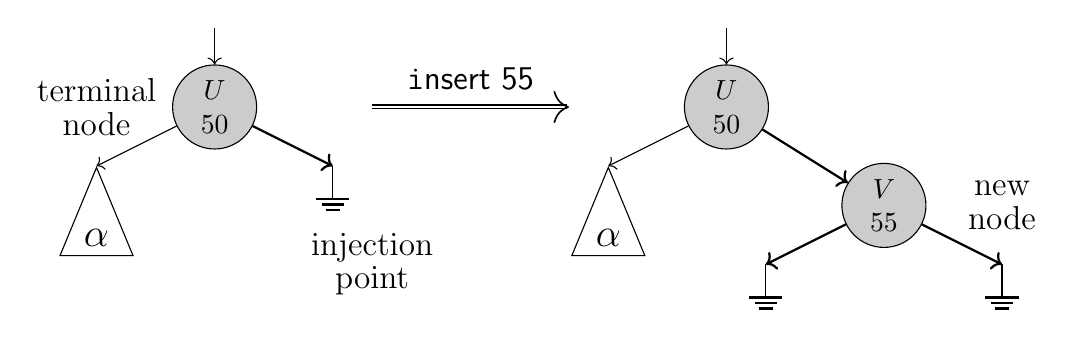
\begin{tikzpicture}
		\newcommand\XA{0}
		\newcommand\YA{0}
		\node (x)		[treenode,fill=black!20] 									at (\XA,\YA)       							{$U$ \\ 50};
		\node (S1)	[subtree] 																at ([shift=({-1.5,-0.75})]x)  	{\Large $\alpha$};
		\node (gnd)	[ground] 																	at ([shift=({1.5,-0.75})]x)			{}; 
		\node (l1) [rectangle,align=center,minimum size=1cm] 	at (\XA-1.5,\YA) 								{\large terminal \\ \large node};
		\node (l2) [rectangle,align=center,minimum size=1cm] 	at (\XA+2,\YA-2.0) 					{\large injection \\ \large point};
		\path[every node/.style={font=\sffamily\small}]
		(\XA,\YA+1) edge[->] 																	node 														{} (x)
		(x) 				edge[->]																	node 														{} (S1.north)
		(x) 				edge[->,thick]														node 														{} (gnd);

		\path[every node/.style={font=\sffamily\small}]
		(\XA+2.0,\YA) edge[->,semithick, double] node [above, outer sep=3pt] {\large \texttt insert 55} (\XA+4.5,\YA);
		\renewcommand\XA{6.5}
		\renewcommand\YA{0}
		\node (x1)		[treenode,fill=black!20] 								at (\XA,\YA)       							{$U$ \\ 50};
		\node (S2)	[subtree] 																at ([shift=({-1.5,-.75})]x1)  	{\Large $\alpha$};
		\node (y)		[treenode,fill=black!20] 									at ([shift=({2,-1.25})]x1)   		{$V$ \\ 55};
		\node (l2) [rectangle,align=center,minimum size=1cm] 	at (\XA+3.5,\YA-1.25) 					{\large new \\ \large node};
    \node (gnd1)	[ground] 																at ([shift=({1.5,-0.75})]y)			{}; 
		\node (gnd2)	[ground] 																at ([shift=({-1.5,-0.75})]y)		{}; 
		
		\path[every node/.style={font=\sffamily\small}]
		(\XA,\YA+1) edge[->] 																	node 														{} (x1)
		(x1) 				edge[->]																	node 														{} (S2.north)
		(x1) 				edge[->,thick]														node 														{} (y)
		(y)         edge[->,thick]                						node          									{} (gnd1)
		(y)         edge[->,thick]                						node          									{} (gnd2);
	\end{tikzpicture}
}
\caption{An illustration of an insert operation.}
\label{fig:icdcn-insert}
\end{figure}
An insert operation ((shown in \figref{icdcn-insert})) starts by invoking seek operation. It returns \false{} if the target key matches the stored key; otherwise, it moves to the execution phase. In the execution phase, it attempts to insert the key into the tree as a child node of the last node in the \accesspath{} using a \CAS{} instruction. If the instruction succeeds, then the operation returns \true{}; otherwise, it restarts by invoking the seek function again.

\paragraph*{Delete} 
\begin{figure}[htp]
\centering
{
	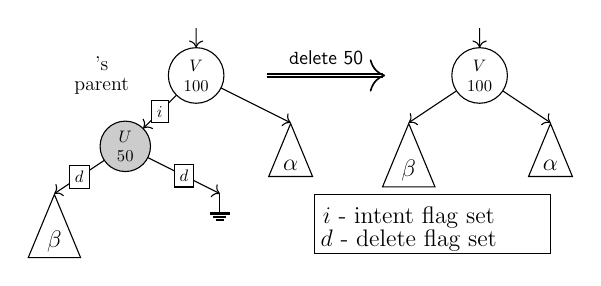
\begin{tikzpicture}[scale=0.6, transform shape,mylabel/.style={thin, draw=black, align=center, minimum width=0.3cm, minimum height=0.3cm,fill=white}]
		\newcommand\XA{-3}
		\newcommand\YA{0}
		\node (x)		[treenode] 																at (\XA,\YA)       					{$V$ \\ 100};
		\node (y)		[treenode, fill=black!20] 								at (\XA-1.5,\YA-1.5) 				{$U$ \\ 50};
		\node (a)		[subtree] 																at (\XA+2,\YA-1)      			{\Large $\alpha$};
		\node (b)		[subtree] 																at (\XA-3,\YA-2.5)    			{\Large $\beta$};
		\node (gnd)	[ground] 																	at (\XA+0.5,\YA-2.5)				{}; 
		\node (xl) 	[rectangle,align=center,minimum size=1cm] at (\XA-2,\YA) 							{\large \targetnode's \\ \large parent};
		\node (yl) 	[] 																				at (\XA-3.25,\YA-1.5) 			{\large \targetnode};
		\draw[->] (x) -- node[mylabel] {$\boldsymbol{i}$} (y);
		\draw[->] (y) -- node[mylabel] {$\boldsymbol{d}$} (b.north);
		\draw[->] (y) -- node[mylabel] {$\boldsymbol{d}$} (gnd);
		\path[every node/.style={font=\sffamily\small}]
		(\XA,\YA+1) edge[->] 																	node 												{} (x)
		%(x) 				edge[->] 																	node[below]  								{\Large $\boldsymbol{i}$} (y)
		(x) 				edge[->] 																	node 				 								{} (a.north);
		%(y) 				edge[->]																	node[below]  								{\Large $\boldsymbol{d}$} (b.north)
		%(y) 				edge[->]																	node[below]  								{\Large $\boldsymbol{d}$} (gnd);

		\path[every node/.style={font=\sffamily\small}]
		(\XA+1.5,\YA) edge[->,semithick, double] 							node [above, outer sep=3pt] {\large \texttt delete 50} (\XA+4,\YA);
		\node (ix)	[treenode] 																at (\XA+6,\YA) 							{$V$ \\ 100};
		\node (ib)	[subtree] 																at (\XA+4.5,\YA-1)					{\Large $\beta$};
		\node (ia)	[subtree] 																at (\XA+7.5,\YA-1) 					{\Large $\alpha$};

		\path[every node/.style={font=\sffamily\small}]
		(\XA+6,\YA+1) 	edge[->] 															node 												{} (ix)
		(ix) 				edge[->] 																	node 												{} (ib.north)
		(ix) 				edge[->] 																	node 												{} (ia.north);

		%% legend
		\node (l1) 																						at (\XA+4.5,\YA-3){\Large $\boldsymbol{i}$  - \Large intent flag set};
		\node (l2) 																						at (\XA+4.5,\YA-3.5){\Large $\boldsymbol{d}$  - \Large delete flag set};
		\node [thin, draw=black, align=center, minimum width=5cm, minimum height=1.25cm] at (\XA+5,\YA-3.15) {};	
	\end{tikzpicture}
}
\caption{An illustration of a simple delete operation.}
\label{fig:simple}
\end{figure}
\begin{figure}[htp]
\centering
{
	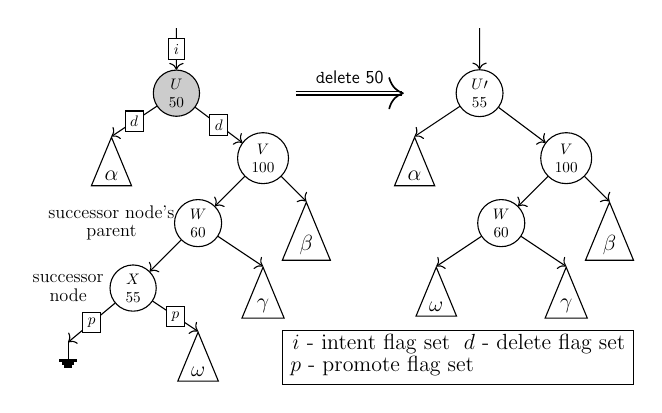
\begin{tikzpicture}[scale=0.55, transform shape,mylabel/.style={thin, draw=black, align=center, minimum width=0.3cm, minimum height=0.3cm,fill=white}]
		\newcommand\XA{0}
		\newcommand\YA{0}
		\node (x)		[treenode, fill=black!20] 	at (-6,0)       							{$U$ \\ 50};
		\node (a)		[subtree] 									at (-7.5,-1)  								{\Large $\alpha$};
		\node (y0)	[treenode] 									at (-4,-1.5) 									{$V$ \\ 100};
		\node (y1)	[treenode]									at (-5.5,-3)									{$W$ \\ 60}; 
		\node (b)		[subtree] 									at (-3,-2.5)    							{\Large $\beta$};
		\node (y2)	[treenode]									at (-7,-4.5)									{$X$ \\ 55}; 
		\node (g)		[subtree] 									at (-4,-4)   									{\Large $\gamma$};
		\node (gnd)	[ground] 										at (-8.5,-5.75)									{}; 
		\node (o)		[subtree] 									at (-5.5,-5.5)  							{\Large $\omega$};
		\node (x1) 	[] 													at (-7.75,0) 									{\large \targetnode};
		\node (y1l) [rectangle,align=center,minimum size=1cm] at (-7.5,-3) 		{\large successor node's \\ \large parent};
		\node (y2l) [rectangle,align=center,minimum size=1cm] at(-8.5,-4.5) 	{\large successor \\ \large node};
		%\node (i)																at (-5.8,1.1)							{\Large $\boldsymbol{i}$};
		%\node (p)																at (-7.75,-5.4)								{\Large $\boldsymbol{p}$};
		
		\draw[->] (-6, 1.5) -- node[mylabel] {$\boldsymbol{i}$} (x);
		\draw[->] (x) -- node[mylabel] {$\boldsymbol{d}$} (y0);
		\draw[->] (x) -- node[mylabel] {$\boldsymbol{d}$} (a.north);
		\draw[->] (y2) -- node[mylabel] {$\boldsymbol{p}$} (gnd);
		\draw[->] (y2) -- node[mylabel] {$\boldsymbol{p}$} (o.north);
		
		
		\path[every node/.style={font=\sffamily\large}]
		%(-6, 1.5) edge[->] 											node 													{} (x)
		%(x) 		edge[->] 												node[below] 									{\Large $\boldsymbol{d}$} (y0)
		%(x) 		edge[->]												node[below] 									{\Large $\boldsymbol{d}$} (a.north)
		(y0) 		edge[->] 												node 													{} (y1)
		(y0) 		edge[->] 												node 													{} (b.north)
		(y1) 		edge[->] 												node 													{} (y2)
		(y1) 		edge[->] 												node 													{} (g.north);
		%(y2) 		edge[->]												node[below] 									{} (gnd)
		%(y2) 		edge[->]												node[below] 									{\Large $\boldsymbol{p}$} (o.north);

		\path[every node/.style={font=\sffamily\small}]
		(-3.25, 0) edge[->,semithick, double] node [above, outer sep=3pt] 		{\large \texttt delete 50} (-0.75, 0);

		\node (ix)	[treenode] 									at (1,0)       								{$U\prime$ \\ 55};
		\node (ia)	[subtree] 									at (-0.5,-1)  								{\Large $\alpha$};
		\node (iy0)	[treenode] 									at (3,-1.5) 									{$V$ \\ 100};
		\node (iy1)	[treenode]									at (1.5,-3)										{$W$ \\ 60}; 
		\node (ib)	[subtree] 									at (4,-2.5)    								{\Large $\beta$};
		\node (io)	[subtree]										at (0,-4)											{\Large $\omega$}; 
		\node (ignd)[subtree] 									at (3,-4)   									{\Large $\gamma$};

		\path[every node/.style={font=\sffamily\small}]
		(1, 1.5) 	edge[->] 											node 													{} (ix)
		(ix) 		edge[->] 												node 													{} (iy0)
		(ix) 		edge[->] 												node 													{} (ia.north)
		(iy0) 	edge[->] 												node 													{} (iy1)
		(iy0) 	edge[->] 												node 													{} (ib.north)
		(iy1) 	edge[->] 												node 													{} (io.north)
		(iy1) 	edge[->] 												node 													{} (ignd.north);

		%% legend
		\node (l1) 															at (-1.5, -5.8)								{\Large $\boldsymbol{i}$  - \Large intent flag set};
		\node (l2) 															at (2.5, -5.8)								{\Large $\boldsymbol{d}$  - \Large delete flag set};
		\node (l3) 															at (-1.25, -6.3)							{\Large $\boldsymbol{p}$  - \Large promote flag set};
		\node [thin, draw=black, align=center, minimum width=8.1cm, minimum height=1.25cm] at (0.5, -6.1) {};
	\end{tikzpicture}
}
\caption{An illustration of a complex delete operation.}
\label{fig:complex}
\end{figure}
A delete operation starts by invoking seek function. It returns \false{} if the stored key does not match the target key; otherwise, it moves to the execution phase. In the execution phase, it attempts to remove the key stored in the \terminalnode{} of the \accesspath. There are two cases depending on whether the \terminalnode{} is a binary node (has two children) or not (has at most one child). In the first case, the operation is referred to as \emph{complex delete operation}. In the second case, it is referred to as \emph{simple delete operation}. In the case of simple delete (shown in \figref{icdcn-simple}), the \terminalnode{} is removed by changing the pointer at the parent node of the \terminalnode. In the case of complex delete (shown in \figref{icdcn-complex}), the key to be deleted is replaced with the \emph{next largest} key in the tree, which will be stored in the \emph{leftmost node} of the \emph{right subtree} of the \terminalnode.

\subsection{Details of the Algorithm}

\begin{figure}[htp]
\centering
{
	\begin{tikzpicture}[scale=0.625, transform shape]
	\newcommand\XA{0}
	\newcommand\YA{0}
	\newcommand\XB{\XA-1}
	\newcommand\YB{\YA-3.8}
	\node (R)			[treenode] 									at (\XA,\YA)       						{$\snodeone$ \\ $\infty$$_0$};
	\node (gnd)		[ground] 										at ([shift=({-1.5,-1})]R)				{};  
	\node (S)			[treenode] 									at ([shift=({1.5,-1.35})]R)			{$\snodetwo$ \\ $\infty$$_1$};
	\node (gndls)	[ground] 										at ([shift=({-1.5,-1})]S)				{}; 
	\node (T)			[treenode] 									at ([shift=({1.5,-1.35})]S)			{$\snodethree$ \\ $\infty$$_2$};
%	\node (gndlt)	[ground] 										at ([shift=({-1,-1})]T)				{};  
	\node (gndt)	[ground] 										at ([shift=({1.5,-1})]T)				{};  


	\path[every node/.style={font=\sffamily\small}]
	(R) 					edge[->] 										node  												{} (S)
	(R) 					edge[->] 										node 				 									{} (gnd)
	(S)						edge[->] 										node 													{} (gndls)
	(S)						edge[->] 										node 													{} (T)
%	(T)						edge[->] 										node 													{} (gndlt)
	(T)						edge[->] 										node 													{} (gndt);
	\renewcommand\XA{0}
	\renewcommand\YA{-4}
	\renewcommand\XB{\XA+2}
	\renewcommand\YB{\YA-6.8}
	\node (x)		[treenode] 									at (\XA,\YA)       						{$U$ \\ 10};
	\node (S1)	[subtree1] 									at ([shift=({-1.5,-0.5})]x)  		{\Large $\alpha$};
	\node (y0)	[treenode] 									at ([shift=({3,-0.5})]x) 			{$V$ \\ 100};
	\node (y1)	[treenode,fill=black!20]		at ([shift=({-1.5,-1})]y0)		{$W$ \\ 60}; 
	\node (S2)	[subtree1] 									at ([shift=({2,-0.5})]y0)   	{$\beta$};
	\node (S3)	[subtree1] 									at ([shift=({-1.5,-1})]y1)  		{\Large $\gamma$};
	\node (y2)	[treenode]									at ([shift=({1.5,-1})]y1)			{$X$ \\ 55}; 
	\node (y3)	[treenode]									at ([shift=({-1,-1.5})]y2)		{$Y$ \\ 50}; 
	\node (S4)	[subtree1] 									at ([shift=({1.5,-0.5})]y2)  	{\Large $\omega$};
	\node (y4)	[treenode,fill=black!20]		at ([shift=({-1,-1.5})]y3)		{$Z$ \\ 40};
	\node (S5)	[subtree1] 									at ([shift=({1.5,-0.5})]y3)  	{\Large $\delta$}; 
	\node (gnd)	[ground] 										at ([shift=({-1,-1})]y4)			{}; 
	\node (S6)	[subtree1] 									at ([shift=({1.5,-0.5})]y4)  	{\Large $\sigma$}; 
	\node (y1l) [rectangle,align=center,minimum size=1cm] at (\XA+0.25,\YA-1.4) 				{\large anchor \\ \large node};
	\node (y4l) [] 													at (\XA-1.0,\YA-5.4) 				{\large \terminalnode};
	\node (x1) 	[rectangle,align=center,minimum size=1cm]at (\XA-1.75,\YA-6.75) 	{\large injection point};

	\path[every node/.style={font=\sffamily\large}]
	%(\XA,\YA+1) 	edge[->,thick] 						node 													{} (x)
	(T)			edge[->,dotted] 								node 													{} (x)
	(x) 		edge[->]												node 													{} (y0)
	(x) 		edge[->]												node 													{} (S1.north)
	(y0) 		edge[->]												node 													{} (y1)
	(y0) 		edge[->]												node 													{} (S2.north)
	(y1) 		edge[->]												node 													{} (S3.north)
	(y1) 		edge[->]												node 													{} (y2)
	(y2) 		edge[->]												node 													{} (y3)
	(y2) 		edge[->]												node 													{} (S4.north)
	(y3) 		edge[->]												node 													{} (y4)
	(y3) 		edge[->]												node 													{} (S5.north)
	(y4) 		edge[->]												node 				 									{} (gnd)
	(y4) 		edge[->]												node 													{} (S6.north);
		
 \end{tikzpicture}
}
\caption{Nodes in the access path of seek along with sentinel keys and nodes ($\infty_0 < \infty_1 < \infty_2$)}
\label{fig:sentinelAndSeek}
\end{figure}



As in most algorithms, we use sentinel keys and three sentinel nodes to handle the boundary cases easily.  The structure of an empty tree with only sentinel keys (denoted by $\skey{0}$, $\skey{1}$ and $\skey{2}$ with $\skey{0} < \skey{1} < \skey{2}$) and sentinel nodes (denoted by $\snodeone$, $\snodetwo$ and $\snodethree$) is shown in \figref{icdcn-sentinelAndSeek}.


Our algorithm, like the one in~\cite{NatMit:2014:PPoPP}, operates at edge level. A delete operation obtains ownership of the edges it needs to work on by marking them. To enable marking, we steal bits from the child addresses of a node. Specifically, we steal \emph{three} bits from each child address to distinguish between three types of marking: 
%%
\begin{enumerate*}[label=(\roman*)]
\item marking for \emph{intent}, 
\item marking for \emph{deletion} and 
\item marking for \emph{promotion}.
\end{enumerate*}
%%
The three bits are referred to as \emph{\intentFlag}, \emph{\deleteFlag} and \emph{\promoteFlag}. To avoid the ABA problem, as in Howley and Jones~\cite{HowJon:2012:SPAA}, we use \emph{unique} null pointers. To that end, we steal another bit from the child address, referred to as \emph{\nullFlag}, and use it to indicate whether the address field contains a null or a non-null value. So, when an address changes from a non-null value to a null value, we only set the \nullFlag{} and the contents of the address field are not otherwise modified. This ensures that all null pointers are unique.

Finally, we also steal a bit from the key field to indicate whether the key stored in a node is the original key or the replacement key. This information is used in a complex delete operation to coordinate helping among processes.


We next describe the details of the seek function, which is used by all operations (search as well as modify) to traverse the tree after which we describe the details of 
the execution phase of insert and delete operations.

\subsubsection{The Seek Phase}
A seek function keeps track of the node in the \accesspath{} at which it took the last ``right turn'' (\emph{i.e.}, it last followed a right edge). Let this ``right turn'' node be referred to as \emph{\anchornode} when the traversal reaches the \terminalnode{}. Note that the \terminalnode{} is the node whose key matched the target key or whose next child edge is set to a null address. For an illustration, please see \figref{icdcn-sentinelAndSeek}. In the latter case (stored key does not match the target key), it is possible that the key may have moved up in the tree. To ascertain that the seek function did not miss the key because it may have moved up during the traversal, we use the following set of conditions that are \emph{sufficient} (but not necessary) to guarantee that the seek function did not miss the key. First, the \anchornode{} is still part of the tree. Second, the key stored in the \anchornode{} has not changed since it first encountered the \anchornode{} during the (current) traversal. To check for the above two conditions, we determine whether the \anchornode{} is undergoing removal (either delete or promote flag set) by examining its right child edge. We discuss the two cases one-by-one.

\begin{enumerate}[leftmargin=*, label=(\alph*), noitemsep]

\item \emph{Right child edge not marked:}
In this case, the \anchornode{} is still part of the tree. We next check whether the key stored in the \anchornode{} has changed. If the key has not changed, then the seek function returns the results of the (current) traversal, which consists of three addresses:
\begin{enumerate*}[label=(\roman*)]
\item the address of the \terminalnode{}, 
\item the address of its parent, and
\item the null address stored in the child field of the \terminalnode{} that caused the traversal to terminate.
\end{enumerate*}
The last address is required to ensure that an insert operation works correctly (specifically to ascertain that the child field of the \terminalnode{} has not undergone any change since the completion of the traversal). We refer to it as the \emph{injection point} of the insert operation. On the other hand, if the key has changed, then the seek function restarts from the root of the tree. 


\item \emph{Right child edge marked:}
In this case, we compare the information gathered in the current traversal about the \anchornode{} with that in the previous traversal, if one exists. Specifically, if the \anchornode{} of the previous traversal is same as that of the current traversal  and the keys found in the \anchornode{} in the two traversals also match, then the seek function terminates, but returns the results of the previous traversal (instead of that of the current traversal). This is because the \anchornode{} was definitely part of the tree during the previous traversal since it was reachable from the root of the tree at the beginning of the current traversal. Otherwise, the seek function restarts from the root of the tree.  
\end{enumerate}

The seek function also keeps track of the \emph{second-to-last} edge in the \accesspath{} (whose endpoints are the parent and grandparent nodes of the \terminalnode), which 
is used for helping, if there is a conflict. For insert and delete operations, we refer to the \terminalnode{} as the \emph{\targetnode}. 

\subsubsection{The Execution Phase of an Insert Operation}

\begin{figure}[htp]
\centering
{
	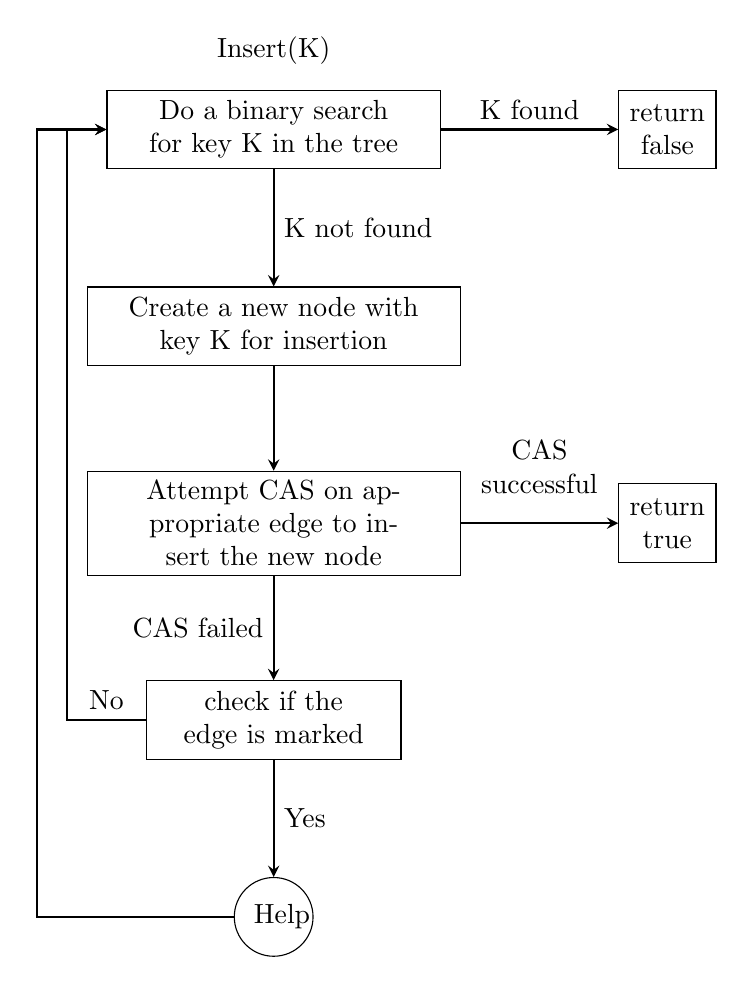
\begin{tikzpicture}
	\node (p0) [] {Insert(K)};
	\node (p1) [process, below of=p0, text width=4cm] {Do a binary search for key K in the tree};
	\node (p2) [process, below of=p1, yshift=-1.5cm, text width=4.5cm] {Create a new node with key K for insertion};
	\node (p3) [process, below of=p2, yshift=-1.5cm, text width=4.5cm] {Attempt CAS on appropriate edge to insert the new node};
	\node (retF) [process, right of=p1, xshift=4cm, text width=1cm, minimum width=1cm] {return false};
	\node (p4) [process, below of=p3, yshift=-1.5cm, text width=3cm] {check if the edge is marked};
	\node (retT) [process, right of=p3, xshift=4cm, text width=1cm, minimum width=1cm] {return true};
	\node (h1) [connector, below of=p4, yshift=-1.5cm] {Help};



	\draw [arrow] (p1) -- node[anchor=west] {K not found} (p2);
	\draw [arrow] (p1) -- node[anchor=south] {K found} (retF);
	\draw [arrow] (p2) -- node {} (p3);
	\draw [arrow] (p3) -- node[anchor=east] {CAS failed} (p4);
	\draw [arrow] (p3) -- node[anchor=south, align=center, yshift=0.25cm] {CAS \\ successful} (retT);
	\draw [arrow] (p4) -- node[anchor=west] {Yes} (h1);
	\draw [arrow] (p4.west) -- ++(-1,0)  node[anchor=south,pos=0.5] {No} |- (p1.west);
	\draw [arrow] (h1.west) -- ++(-2.5,0) |- node[anchor=south] {} (p1.west);
	\end{tikzpicture}
}
\caption{\ICDCN{} - Sequence of steps in an insert operation \label{fig:icdcn-flowInsert}}
\end{figure}
In the execution phase, an insert operation creates a new node containing the target key. It then adds the new node to the tree at the injection point using a \CAS{} instruction. If the \CAS{} instruction succeeds, then (the new node becomes a part of the tree and) the operation terminates; otherwise, the operation determines if it failed because of a \emph{conflicting} delete operation in progress. If there is no conflicting delete operation in progress, then the operation restarts from the seek phase; otherwise it performs helping and then restarts from the seek phase. \figref{icdcn-flowInsert} shows a  flow chart describing the sequence of steps of an insert operation.

\subsubsection{The Execution Phase of a Delete Operation}
The execution of a delete operation starts in \emph{\injection{} mode}. Once the operation has been injected into the tree, it advances to either \emph{\discovery{} mode} or \emph{\cleanup{} mode} depending on the type of the delete operation.


\paragraph*{Injection Mode}

In the \injection{} mode, the delete operation marks the three edges involving the \targetnode{} as follows:
%%
\begin{enumerate*}[label=(\roman*)]
\item It first sets the \intentFlag{} on the edge from the parent of the \targetnode{} to the \targetnode{} using a \CAS{} instruction.
\item It then sets the \deleteFlag{} on the left edge of the \targetnode{} using a \CAS{} instruction.
\item Finally, it sets the \deleteFlag{} on the right edge of the \targetnode{} using a \CAS{} instruction.
\end{enumerate*}
%%
If the \CAS{} instruction fails at any step, the delete operation performs helping, and either repeats the same step or restarts from the seek phase. Specifically, the delete operation repeats the same step when setting the \deleteFlag{} as long as the \targetnode{} has not been claimed as the successor node by another delete operation. In all other cases, it restarts from the seek phase.


We maintain the invariant that an edge, once marked, cannot be unmarked. After marking both the edges of the \targetnode{}, the operation checks whether the \targetnode{} is a binary node or not. If it is a binary node, then the delete operation is classified as complex; otherwise it is classified as simple. Note that the type of the delete operation cannot change once all the three edges have been marked as described above. If the delete operation is complex, then it advances to the \discovery{} mode after which it will advance to the \cleanup{} mode. On the other hand, if it is simple, then it directly advances to the \cleanup{} mode (and skips the \discovery{} mode). Eventually, the \targetnode{} is either removed from the tree (if simple delete) or replaced with a ``new'' node containing the next largest key (if complex delete). 

For a tree node $X$, let $X.\myparent$ denote its parent node, and $X.\myleft$ and $X.\myright$ denote its left and right child node, respectively. Also, hereafter in this section, let $T$ denote the \targetnode{} of the delete operation under consideration.

\paragraph*{Discovery Mode}
In the \discovery{} mode, a complex delete operation  performs the following steps:
%%
\begin{enumerate}[leftmargin=*, noitemsep]
%%
\item \textbf{Find Successor Key:} The operation locates the next largest key in the tree, which is the smallest key in the subtree rooted at the right child of $T$. We refer to this key as the \emph{successor key} and the node storing this key as the \emph{successor node}. Hereafter in this section, let $S$ denote the successor node. 
%%
\item \textbf{Mark Child Edges of Successor Node:} The operation sets the \promoteFlag{} on both the child edges of $S$ using a \CAS{} instruction. Note that the left child edge of $S$ will be null.  As part of marking the left child edge, we also store the address of $T$ (the \targetnode{}) in the edge. This is done to enable helping in case the successor node is obstructing the progress of another operation. 
%%
In case the \CAS{} instruction fails while marking the left child edge, the operation repeats from step~1 after performing helping if needed. On the other hand, if the \CAS{} instruction fails while marking the right child edge, then the marking step is repeated after performing helping if needed. 

%%
\item \textbf{Promote Successor Key:} The operation replaces the \targetnode's original key with the successor key. At the same time, it also sets the mark bit in the key to indicate that the current key stored in the \targetnode{} is the replacement key and not the original key.
%%
\item \textbf{Remove Successor Node:}  The operation removes $S$ (the successor node) by changing the child pointer at$S.\myparent$ that is pointing to $S$ to point to the right child of $S$ using a \CAS{} instruction. If the \CAS{} instruction succeeds, then the operation advances to the \cleanup{} mode. Otherwise, it performs helping if needed. It then finds $S$ again by performing another traversal of the tree starting from the right child of $T$. If the traversal fails to find $S$ (recall that the left edge of $S$ is marked for promotion and contains the address of $T$), then $S$ has already been removed from the tree by another operation as part of helping, and the delete operation advances to the \cleanup{} mode. On advancing to the \cleanup{} mode, the operation sets a flag in $T$  indicating that $S$ has been removed from the tree (and $T$ can now be replaced with a new node) so that other operations trying to help it know not to look for $S$.
\end{enumerate}

\figref{icdcn-flowDelete} shows a  flow chart describing the sequence of steps of a delete operation.
\begin{figure}[htp]
\centering
{
	\begin{tikzpicture}[scale=0.75, transform shape]
		\node (p0) 		{Delete(K)};
		\node (p1) 		[process, below of=p0, text width=6cm] {Do a binary search for key K in the tree};
		\node (p2) 		[process, below of=p1, yshift=-2cm, text width=6cm] {Mark left child edge for delete using CAS};
		\node (p3) 		[process, below of=p2, yshift=-2cm, text width=6cm] {Mark right child edge for delete using BTS. Check the children edges to determine simple or complex delete};
		\node (retF) 	[process, right of=p1, xshift=5.0cm, text width=1cm, minimum width=1cm] {return false};
		\node (p4) 		[process, below of=p3, yshift=-2cm, text width=6cm] {Attempt CAS to change the edge (parent, target node) to point to the non-null child};
		\node (retT) 	[process, right of=p4, xshift=5.0cm, text width=1cm, minimum width=1cm] {return true};
		%\node (C) 		[connector, right of=p3, xshift=5.5cm] {C};
		\node (h1) 		[connector, right of=p2, xshift=5.0cm] {Help};
		\node (h2) 		[connector, below of=p4, yshift=-2cm] {Help};



		\draw [arrow] (p1) -- node[anchor=west] {K found} (p2);
		\draw [arrow] (p1) -- node[anchor=south] {K not found} (retF);
		\draw [arrow] (p2) -- node[anchor=west, align=center] {CAS successful} (p3);
		\draw [arrow] (p2) -- node[anchor=south, align=center, yshift=0.25cm] {CAS \\ failed} (h1);
		\draw[-latex] (h1) to [out=90,in=330,looseness=1] (p1.east);
		\draw [arrow] (p3) -- node[anchor=east] {simple} (p4);
		%\draw [arrow] (p3) -- node[anchor=south] {Complex} (C);
		\draw [arrow] (p4) -- node[anchor=south, align=center, yshift=0.25cm] {CAS \\ successful} (retT);
		\draw [arrow] (p4) -- node[anchor=east] {CAS failed} (h2);
		%\draw [arrow] (h2.west) -- ++(-0,0) |- node[anchor=south] {} (p4.west);
		\draw[-latex] (h2.east) to [out=0,in=0,looseness=1.5] (p4.east);
	%\end{tikzpicture}

	%\begin{tikzpicture}[scale=0.7, transform shape]
	%\node (C) [connector,xshift=11cm] {C};
	%\node (p1) [process, below of=C, yshift=-2cm, text width=6cm] {Find Successor: smallest key in the right subtree};
	\node (p1c) [process, xshift=11cm,text width=6cm] {Find Successor: smallest key in the right subtree};
	\draw [arrow] (p3.east) -- ++(4,0) |- node[anchor=south] {Complex} (p1c.west);
	\node (p2) [process, below of=p1c, yshift=-2cm, text width=6cm] {Mark left child edge for promotion using CAS};
	\node (p3) [process, below of=p2, yshift=-2cm, text width=6cm] {Mark right child edge for promotion using BTS. Promote successor's key by copying it to the target node using a simple write};
	\node (h1) [connector, right of=p2, xshift=5cm] {Help};
	\node (p4) [process, below of=p3, yshift=-2cm, text width=6cm] {Attempt CAS to change the edge (successor parent,successor) to point to the right child of successor};
	\node (p5) [process, below of=p4, yshift=-2cm, text width=6cm] {Create a fresh copy of the target node with the new key and its children edges unmarked};
	\node (h2) [connector, right of=p4, xshift=5cm] {Help};
	\node (p6) [process, below of=p5, yshift=-2cm, text width=6cm] {Attempt CAS to change the edge (parent, target node) to point to the new node};
	\node (retT) [process, below of=p6, yshift=-2cm, text width=1cm, minimum width=1cm] {return true};
	\node (h3) [connector, right of=p6, xshift=5cm] {Help};

	%\draw [arrow] (C) -- node[] {} (p1);
	\draw [arrow] (p1c) -- node[] {} (p2);
	\draw [arrow] (p2) -- node[anchor=east] {CAS successful} (p3);
	\draw [arrow] (p2) -- node[anchor=south, yshift=0.5cm] {CAS failed} (h1);
	\draw [arrow] (h1.north)  |-  node[] {} (p1c.east);
	\draw [arrow] (p3) -- node[] {} (p4);
	\draw [arrow] (p4) -- node[anchor=east] {CAS successful} (p5);
	\draw [arrow] (p4) -- node[anchor=south] {CAS failed} (h2);
	\draw[-latex] (h2) to [out=270,in=330,looseness=1] (p4.east);
	\draw [arrow] (p5) -- node[] {} (p6);

	\draw [arrow] (p6) -- node[anchor=south] {CAS failed} (h3);
	\draw[-latex] (h3) to [out=270,in=330,looseness=1] (p6.east);
	\draw [arrow] (p6) -- node[anchor=east] {CAS successful} (retT);

	\end{tikzpicture}
\caption{\ICDCN{} - Sequence of steps in a delete operation \label{fig:icdcn-flowDelete}}
}
\end{figure}



\begin{limitscope}

%% To limit the scope of the macros defined below

%% macros for pseudocode
\newcommand{\leftChild}{le\!f\!t}
\newcommand{\rightChild}{right}
\newcommand{\child}{child}
\newcommand{\canReplace}{readyToReplace}
\newcommand{\markAndKey}{mKey}

\newcommand{\node}{node}
\newcommand{\parent}{parent}

\newcommand{\terminalEdge}{lastEdge}
\newcommand{\targetEdge}{targetEdge}
\newcommand{\parentTargetEdge}{pTargetEdge}
\newcommand{\successorEdge}{successorEdge}
\newcommand{\parentSuccessorEdge}{pSuccessorEdge}
\newcommand{\injectionEdge}{injectionEdge}
\newcommand{\penultimateEdge}{pLastEdge}

\newcommand{\targetKey}{targetKey}
\newcommand{\currentKey}{currentKey}

\newcommand{\newNode}{newNode}
\newcommand{\reference}{re\!f\!erence}
\newcommand{\state}{state}

\newcommand{\StateRecord}{StateRecord}
\newcommand{\AnchorRecord}{AnchorRecord}

\newcommand{\mline}[1]{\DontPrintSemicolon #1 \PrintSemicolon}

\newcommand{\prev}{prev}
\newcommand{\curr}{curr}

\newcommand{\prevSeekRecord}{pSeekRecord}
\newcommand{\prevAnchorRecord}{pAnchorRecord}
%% \newcommand{\currSeekRecord}{cSeekRecord}
\newcommand{\anchorRecord}{anchorRecord}

\newcommand{\oldContents}{oldValue}
\newcommand{\newContents}{newValue}

\newcommand{\INJECTION}{\textsf{INJECTION}}
\newcommand{\DISCOVERY}{\textsf{DISCOVERY}}
\newcommand{\CLEANUP}{\textsf{CLEANUP}}
\newcommand{\FINISHED}{\textsf{FINISHED}}

\newcommand{\DELETEFLAG}{\textsf{DELETE\_FLAG}}
\newcommand{\PROMOTEFLAG}{\textsf{PROMOTE\_FLAG}}
\newcommand{\INTENTFLAG}{\textsf{INTENT\_FLAG}}
\newcommand{\flag}{f\!lag}

\newcommand{\COMPLEX}{\textsf{COMPLEX}}
\newcommand{\SIMPLE}{\textsf{SIMPLE}}

\newcommand{\LEFT}{\textsf{LEFT}}
\newcommand{\RIGHT}{\textsf{RIGHT}}

\newcommand{\targetSeekRecord}{targetRecord}
\newcommand{\successorSeekRecord}{successorRecord}

\newcommand{\dFlag}{d}
\newcommand{\iFlag}{i}
\newcommand{\pFlag}{p}
\newcommand{\nFlag}{n}
\newcommand{\mFlag}{m}
\newcommand{\lNFlag}{lN}
\newcommand{\rNFlag}{rN}

\newcommand{\rarrow}{\!\rightarrow\!}


%%%%%%%%%%%%%%%%%%%%%%%%%%%%%%%%%%%%%%%%%%%%%%%%%%%%%%%%%%%%%%%%%%%%%%%%%%%%%%%%%%%%

\newcommand{\DefineKeyWords}{
%%
\SetKw{Boolean}{Boolean}
\SetKw{LAnd}{~and~}
\SetKw{LOr}{~or~}
\SetKw{LNot}{not}
\SetKw{Struct}{struct}
\SetKw{Null}{null}
\SetKw{True}{true}
\SetKw{False}{false}
\SetKw{Break}{break}
\SetKw{Continue}{continue}
\SetKw{Enum}{enum}
%%
}

%%%%%%%%%%%%%%%%%%%%%%%%%%%%%%%%%%%%%%%%%%%%%%%%%%%%%%%%%%%%%%%%%%%%%%%%%%%%%%%%%%%%%

%% DATA STRUCTURES


\begin{algorithm}[htp]
%%
\DefineKeyWords
%%

%% define data structures used in the algorithm

\DontPrintSemicolon
\Struct Node \{\;
\label{ln:icdcn-node|begin}
\PrintSemicolon
\Indp 
   $\{ \Boolean, \text{Key} \}$ $\markAndKey$\;
   $\{ \Boolean, \Boolean, \Boolean, \Boolean, \text{NodePtr} \}$ $\child[2]$\;
   \Boolean $\canReplace$\;
\Indm
\}\;
\label{ln:icdcn-node|end}
%%
\BlankLine

\DontPrintSemicolon
\Struct Edge \{\;
\label{ln:icdcn-edge|begin}
\PrintSemicolon
\Indp 
   %% NodePtr $\parent$\;
   %% NodePtr $\child$\;
	 NodePtr $\parent$, $\child$\;
   \Enum $which$ \{ \LEFT{}, \RIGHT{} \}\;
\Indm
\}\;
\label{ln:icdcn-edge|end}
%%
\BlankLine

\DontPrintSemicolon
\Struct SeekRecord \{\;
\PrintSemicolon
\Indp 
%%
   %% Edge $\terminalEdge$\;
%%
   %% Edge $\penultimateEdge$\;
%%
   %% Edge $\injectionEdge$\;
   Edge $\terminalEdge$, $\penultimateEdge$, $\injectionEdge$\;
\Indm
\}\;
%%
\BlankLine


\BlankLine
\DontPrintSemicolon
\Struct \AnchorRecord{} \{\;
\PrintSemicolon
\Indp 
   NodePtr $\node$\;
   Key $key$\;
\Indm
\}\;
%%

\BlankLine
\DontPrintSemicolon
\Struct \StateRecord{} \{\;
\PrintSemicolon
\Indp 
%%
   %% int $depth$\;
   %% Edge $\targetEdge$\;
	 %% Edge $\parentTargetEdge$\;
	 Edge $\targetEdge$, $\parentTargetEdge$\;
%%
   %% Key $\targetKey$\;
	 %% Key $\currentKey$\;
	 Key $\targetKey$, $\currentKey$\;
   \Enum $mode$ \{ \INJECTION{}, \DISCOVERY{}, \CLEANUP{} \}\;
   \Enum $type$ \{ \SIMPLE{}, \COMPLEX{} \} \;
%%
   \tcp{the next field stores pointer to a seek record; it is used for finding the successor if the delete operation is complex}
   SeekRecordPtr $\successorSeekRecord$\; 
\Indm
\}\;
%%
\BlankLine
\tcp{object to store information about the tree traversal when looking for a given key (used by the seek function)}
SeekRecordPtr $\targetSeekRecord$ := new seek record\;
\tcp{object to store information about process' own delete operation}
\StateRecord{Ptr} $myState$ := new state\;


\caption{Data Structures Used}
\label{algo:icdcn-data|structures}
\end{algorithm}



\begin{algorithm}[htp]
%%
\DefineKeyWords


%% SEEK


%%
%% traverses the tree from the root node to a leaf node looking for a given key
%%
\DontPrintSemicolon
\Seek( $key$, $seekRecord$ )\;
\PrintSemicolon
\Begin
{
   $\prevAnchorRecord$ := $\curly{ \snodetwo{}, \skey{1} }$\;
   \While{\True}
   {
	    \tcp{initialize all variables used in traversal}
		  $\penultimateEdge$ := $\curly{ \snodeone, \snodetwo, \RIGHT }$; \qquad
			$\terminalEdge$ := $\curly{ \snodetwo, \snodethree, \RIGHT }$\;
			$\curr$ := $\snodethree$; \qquad
			$\anchorRecord$ := $\curly{ \snodetwo{}, \skey{1} }$\;
			\BlankLine
			\While{\True}
			{
			    \tcp{read the key stored in the current node}
			    $\ang{ \ast, cKey }$ := $\curr \rarrow \markAndKey$\;
				  \tcp{find the next edge to follow}
					$which$ := $key < cKey$ ? \LEFT : \RIGHT\;
				  $\ang{ \nFlag, \ast, \dFlag, \pFlag, next }$ := $\curr \rarrow \child[which]$\;
					\tcp{check for the completion of the traversal}
				  \If{$key = cKey$ \LOr $\nFlag$}
				  {
				     \tcp{either key found or no next edge to follow; stop the traversal}
						 $seekRecord \rarrow \penultimateEdge$ := $\penultimateEdge$\;
						 $seekRecord \rarrow \terminalEdge$ := $\terminalEdge$\;
						 $seekRecord \rarrow \injectionEdge$ := $\curly{ \curr, next, which }$\;
						 \BlankLine
						 \uIf(\tcp*[h]{keys match}){$key = cKey$}
						 { 
						    \Return\;
						 }
						 \lElse { \Break }
				  }
				  \BlankLine			   
				  \If{$which$ = \RIGHT}
				  {
				     \tcp{next edge to be traversed is a right edge; keep track of the current node and its key}
						 $\anchorRecord$ := $\ang{ \curr, cKey }$\;
				  }	
				  \BlankLine
				  \tcp{traverse the next edge}
					$\penultimateEdge$ := $\terminalEdge$; \qquad
					$\terminalEdge$ := $\curly{ \curr, next, which }$; \qquad
				  $\curr$ := $next$\; 
		  }
		  \tcp{key was not found; check if can stop}
		  $\ang{ \ast, \ast, \dFlag, \pFlag, \ast }$ := $\anchorRecord.\node \rarrow \child[\RIGHT]$\;			
			\uIf{\LNot($\dFlag$) \LAnd \LNot($\pFlag$)}
			{
			   \tcp{anchor node is still part of the tree; check if anchor node's key has changed}
				 $\ang{ \ast, aKey }$ := $\anchorRecord.\node \rarrow \markAndKey$\;
				 \lIf{$\anchorRecord.key$ = $aKey$}
			   {  
				    \Return
				 } 
			}	
			\Else
			{ 
			   \tcp{check if the anchor record (the node and its key) matches that of the previous traversal}
			   \If{$\prevAnchorRecord = \anchorRecord$}
			   {
				    \tcp{return the results of the previous traversal}
					  $seekRecord$ := $\prevSeekRecord$\;
				    \Return\;
		     }
			}
			\tcp{store the results of the traversal and restart}
			$\prevSeekRecord$ := $seekRecord$; \qquad
			$\prevAnchorRecord$ := $\anchorRecord$;					
   }
} 
%% End of seek function
\caption{Seek Function}
\label{algo:icdcn-seek}
\end{algorithm}


%% SEARCH
\begin{algorithm}[htp]
%%
\DefineKeyWords
\DontPrintSemicolon
\Boolean \Search( $key$ )\;
\PrintSemicolon
\Begin
{
   \Seek( $key$, $mySeekRecord$ )\;
	 \BlankLine
	 %% $\node$ := $mySeekRecord \rarrow \node$\;
   $\node$ := $mySeekRecord \rarrow \terminalEdge.\child$\;
   $\ang{ \ast , nKey }$ := $\node \rarrow \markAndKey$\;
	 \BlankLine
   \lIf{nKey = key}{\Return \True}
   \lElse{\Return \False}
}
\caption{Search Operation}
\label{algo:icdcn-search}
\end{algorithm}

%% INSERT
\begin{algorithm}[htp]
%%
\DefineKeyWords
\DontPrintSemicolon
\Boolean \Insert( $key$ )\;
\PrintSemicolon
\Begin
{
   \While{\True}
	 {
      \Seek( $key$, $\targetSeekRecord$ )\;
			\BlankLine
			$\targetEdge$ := $\targetSeekRecord \rarrow \terminalEdge$\;
			$\node$ := $\targetEdge.\child$\;
			$\ang{ \ast , nKey }$ := $\node \rarrow \markAndKey$\; 
			\lIf{$key = nKey$}{\Return \False}
			\BlankLine
			\tcp{create a new node and initialize its fields}
			$\newNode$ := create a new node\;
			$\newNode \rarrow \markAndKey$ := $\ang{ 0_m, key }$\;
			$\newNode \rarrow \child[\LEFT]$ := $\ang{ 1_n, 0_i, 0_d, 0_p, \Null }$\;
			$\newNode \rarrow \child[\RIGHT]$ := $\ang{ 1_n, 0_i, 0_d, 0_p, \Null }$\;
			$\newNode \rarrow \canReplace$ := \False\;
			\BlankLine
			$which$ := $\targetSeekRecord \rarrow \injectionEdge.which$\;
			$address$ := $\targetSeekRecord \rarrow \injectionEdge.\child$\;
			$result$ := \CAS($\node \rarrow \child[which]$, $\ang{ 1_n, 0_i, 0_d, 0_p, address }$, $\ang{ 0_n, 0_i, 0_d, 0_p, \newNode }$)\;
			\lIf{$result$}{\Return \True}
			\BlankLine	
			\tcp{help if needed}
		  $\ang{ \ast, \ast, \dFlag, \pFlag, \ast }$ := $\node \rarrow \child[which]$\;
			\lIf{$\dFlag$}
			{
			   \HelpTargetNode( $\targetEdge$ )
			} 
			\lElseIf{$p$}
			{  
			   \HelpSuccessorNode( $\targetEdge$ )
			}
	}
}
\caption{Insert Operation}
\label{algo:icdcn-insert}
\end{algorithm}

%% DELETE
\begin{algorithm}[htp]
\DefineKeyWords
\DontPrintSemicolon
\Boolean \Delete( $key$ )\;
\PrintSemicolon
\Begin
{
   \tcp{initialize the state record}
 	 $myState \rarrow \targetKey$ := $key$; $\qquad$
	 $myState \rarrow \currentKey$ := $key$\;
	 $myState \rarrow mode$ := \INJECTION\;
	 \BlankLine
   \While{\True}
	 {
      \Seek( $myState \rarrow \currentKey$, $\targetSeekRecord$ )\;
			$\targetEdge$ := $\targetSeekRecord \rarrow \terminalEdge$; $\qquad$
			$\parentTargetEdge$ := $\targetSeekRecord \rarrow \penultimateEdge$\;
			$\ang{ \ast , nKey }$ := $\targetEdge.\child \rarrow \markAndKey$\; 
			\BlankLine
			\If{$myState \rarrow \currentKey \neq nKey$}
			{
			   \tcp{the key does not exist in the tree}
			   \lIf{$myState \rarrow mode$ = \INJECTION}{\Return \False}
				 \lElse{\Return \True}
			}
 	    \BlankLine		   	
			\tcp{perform appropriate action depending on the mode}
	    \If{$myState \rarrow mode$ = \INJECTION}
		  {
				 \tcp{store a reference to the target edge}
   	     $myState \rarrow \targetEdge$ := $\targetEdge$\;
   	     $myState \rarrow \parentTargetEdge$ := $\parentTargetEdge$\;
				 \tcp{attempt to inject the operation at the node}
				 %% $result$ := \Inject( $myState$ )\;
				 \Inject( $myState$ )\;					 								 
			}
			\BlankLine
			\tcp{mode would have changed if injection was successful}
				 
			\If{$myState \rarrow mode \neq$ \INJECTION}
			{
				 \tcp{check if the target node found by the seek function matches the one stored in the state record}			
			   %%\If{$\left(\text{\parbox[c]{1.75in}{$myState \rarrow \targetEdge.\child$ $\neq$  \\ \mbox{}\hfill$\targetEdge.\child$}}\right)$}
				 \lIf{$myState \rarrow \targetEdge.\child$ $\neq$ $\targetEdge.\child$}
				 {
				    \Return \True
				 }						
				 \tcp{update the target edge information using the most recent seek}
				 $myState \rarrow \targetEdge$ := $\targetEdge$\; 			 				
		  }				
			\BlankLine							
			\If{$myState \rarrow mode$ = \DISCOVERY}
			{
				 \tcp{complex delete operation; locate the successor node and mark its child edges with promote flag} 
			   \FindAndMarkSuccessor( $myState$ )\;			 
			}			
			\If{$myState \rarrow mode$ = \DISCOVERY}
			{
				 \tcp{complex delete operation; promote the successor node's key and remove the successor node}
		     \RemoveSuccessor( $myState$ )\;						
			}			
			\BlankLine				
			\If{$myState \rarrow mode$ = \CLEANUP}
			{
			   \tcp{either remove the target node (simple delete) or replace it with a new node with all fields unmarked  (complex delete)}
			   $result$ := \Cleanup( $myState$ )\;
				 \lIf{$result$}{\Return \True}
				 \Else{
				    $\ang{ \ast, nKey }$ := $\targetEdge.\child \rarrow \markAndKey$\;
						$myState \rarrow \currentKey$ := $nKey$\;
				 }					
		  }
	 }	
   %% \Return\;
}
\caption{Delete Operation}
\label{algo:icdcn-delete}
\end{algorithm}

%% INJECT
\begin{algorithm}[htp]
%%
\DefineKeyWords
\DontPrintSemicolon
\Inject( $\state$ )\;
\PrintSemicolon
\Begin
{
   $\targetEdge$ := $\state \rarrow \targetEdge$\;
	 \tcp{try to set the intent flag on the target edge}
	 \tcp{retrieve attributes of the target edge}
	 $\parent$ := $\targetEdge.\parent$\;
	 $\node$ := $\targetEdge.\child$\;
	 $which$ := $\targetEdge.which$\;
	 \BlankLine
	 \mline{$result$ := \CAS( \parbox[t]{2.075in}{$\parent \rarrow \child[which]$, \\ $\ang{ 0_n, 0_i, 0_d, 0_p, \node }$,  $\ang{ 0_n, 1_i, 0_d, 0_p, \node }$ );}\;}
	 \If{\LNot($result$)}
	 {
	    \tcp{unable to set the intent flag; help if needed}
			$\ang{ \ast, \iFlag, \dFlag, \pFlag, address }$ := $\parent \rarrow \child[which]$\;
			\lIf{$\iFlag$}
			{
			   \HelpTargetNode( $\targetEdge$ )
			} 
			\uElseIf{$\dFlag$}
			{
			   \HelpTargetNode( $\state \rarrow \parentTargetEdge$ )\;
			} 
			\ElseIf{$\pFlag$}
			{
			   \HelpSuccessorNode( $\state \rarrow \parentTargetEdge$ )\;
			}

      \Return;					
	 }

   \BlankLine
	 \tcp{mark the left edge for deletion}

	 $result$ := \MarkChildEdge( $\state$, \LEFT{} )\;
	 
	 \lIf{\LNot($result$)}
	 {
	    \Return
	 } 
	 \tcp{mark the right edge for deletion; cannot fail}
	 \MarkChildEdge( $\state$, \RIGHT{} )\;
	   
	 \BlankLine
	 \tcp{initialize the type and mode of the operation}
	 \InitializeTypeAndUpdateMode( $\state$ );	
}

\caption{Injecting a Deletion Operation}
\label{algo:icdcn-inject}
\end{algorithm}









%% FINDANDMARKSUCCESSOR


\begin{algorithm}[htp]
%%
\DefineKeyWords

\DontPrintSemicolon
\FindAndMarkSuccessor( $\state$ )\;
\PrintSemicolon
\Begin
{
   \tcp{retrieve the addresses from the state record}
   $\node := \state \rarrow \targetEdge.\child$\;
	 $seekRecord$ := $\state \rarrow \successorSeekRecord$\; 
   
	 \BlankLine
   \While{\True}
	 {
	 
	    \tcp{read the mark flag of the key in the target node}  
	    $\ang{ \mFlag, \ast}$ := $\node \rarrow \markAndKey$\; 
	    

	  	\tcp{find the node with the smallest key in the right subtree}
	    $result$ := \FindSmallest( $\state$ )\;
			
						
			\BlankLine
			\If{$\mFlag$ \LOr \LNot($result$)} 
			{
			   \tcp{successor node had already been selected \emph{before} the traversal or the right subtree is empty}
				 \Break\;
			}
			
				
			\tcp{retrieve the information from the seek record}
			$\successorEdge$ := $seekRecord \rarrow \terminalEdge$\;
			%% $\ang{ \nFlag, \ast, \ast, \ast, \leftChild}$ :=  $\successorEdge.\child \rarrow \child[\LEFT]$\;
			%% \lIf{\LNot($\nFlag$)}{ \Continue }
			$\leftChild$ := $seekRecord \rarrow \injectionEdge.\child$\;
			
			\BlankLine
			\tcp{read the mark flag of the key under deletion}
      $\ang{ \mFlag, \ast}$ := $\node \rarrow \markAndKey$\;
			
			\If(\tcp*[h]{successor node has already been selected}){$\mFlag$}
			{
			   %% \tcp{successor node has already been selected}
			   %% \lIf{$p$}{ \Break }
				 %% \lElse{ \Continue }
				 \Continue\;
				 
			}
			
			
		


          
			\tcp{try to set the promote flag on the left edge}
			\mline{$result$ := \CAS( \parbox[t]{1.875in}{$\successorEdge.\child \rarrow \child[\LEFT]$, \\ 
			                                             $\ang{ 1_n, 0_i, 0_d, 0_p, \leftChild }$, \\ $\ang{ 1_n, 0_i, 0_d, 1_p, \node }$ );}\;}
			
			\lIf{$result$}{\Break}
			
			\BlankLine
			\tcp{attempt to mark the edge failed; recover from the failure and retry if needed}
			%% $\ang{ n, \ast, d, p, \ast }$ := $\successorEdge.\child \rarrow \child[\LEFT]$\;
			$\ang{ \nFlag, \ast, \dFlag, \ast, \ast }$ := $\successorEdge.\child \rarrow \child[\LEFT]$\;
			
			
      %% \lIf{$p$}
      %% {
      %%    \Break
      %% }   

      %% \If{\LNot($n$)}
			%% { 
			%%   \tcp{the node found has since gained a left child}
			%%   \Continue\;
			%% }

			\If{$\nFlag$ \LAnd $\dFlag$}
			{
			    \tcp{the node found is undergoing deletion; need to help}
					
								
					%% \mline{\HelpTargetNode( \parbox[t]{1.5in}{$\successorEdge$, \\ $\state \rarrow depth + 1$ );}\;}
		      \HelpTargetNode( $\successorEdge$ )\;
       } 
	 }	
   \BlankLine
   \tcp{update the operation mode}
	 \UpdateMode( $\state$ );
}

\caption{Locating the Successor Node}
\label{algo:icdcn-findandmark}
\end{algorithm}




%% REMOVESUCCESSOR
\begin{algorithm}[htp]
%%
\DefineKeyWords
\DontPrintSemicolon
\RemoveSuccessor( $\state$ )\;
\PrintSemicolon
\Begin
{
   \tcp{retrieve addresses from the state record}
   $\node$ := $\state \rarrow \targetEdge.\child$\;
   $seekRecord$ := $\state \rarrow \successorSeekRecord$\;
   \tcp{extract information about the successor node}
	 %% \tcp{assumes that the state's seek record contains valid information}
   $\successorEdge$ := $seekRecord \rarrow \terminalEdge$\;
	 \BlankLine
	 \tcp{ascertain that seek record for successor node contains valid information}
	 $\ang{ \ast, \ast, \ast, \pFlag, address }$ := $\successorEdge.\child \rarrow \child[\LEFT]$\;
	 \If{\LNot($\pFlag$) \LOr ($address$ $\neq$ $\node$)}
	 {
	    $\node \rarrow \canReplace$ := \True\;
			\UpdateMode( $\state$ )\;
	    \Return\;
	 }
   \BlankLine
   \tcp{mark the right edge for promotion if unmarked}
   \MarkChildEdge( $\state$, \RIGHT{} )\; 
   \BlankLine
   \tcp{promote the key}
   $\node \rarrow \markAndKey$ := $\ang{ 1_m, \successorEdge.\child \rarrow \markAndKey }$\;
   \While{\True}
   {
      \tcp{check if the successor is the right child of the target node itself}
	    \uIf{$\successorEdge.\parent$ = $\node$}
	    {
	       \tcp{need to modify the right edge of target node whose delete flag is set}
				 $dFlag$ := 1; \qquad
			   $which$ := \RIGHT\;
	    }
	    \Else
	    {
			   $dFlag$ := 0; \qquad
			   $which$ := \LEFT\;
	    }
      $\ang{ \ast, \iFlag, \ast, \ast, \ast }$ := $\successorEdge.\parent \rarrow \child[which]$\;			
      \BlankLine			
	    $\ang{ \nFlag, \ast, \ast, \ast, \rightChild }$ := $\successorEdge.\child \rarrow \child[\RIGHT]$\;	
	    $\oldContents$ := $\ang{ 0_n, \iFlag, dFlag, 0_p, \successorEdge.\child }$\;	    
			\uIf(\tcp*[f]{only set the null flag; do not change the address}){$\nFlag$}
	    {				
				 %\mline{\parbox[t]{1.75in}{$\newContents$ := \\ \mbox{} \qquad $\ang{ 1_n, 0_i, dFlag, 0_p,  \successorEdge.\child }$;}}
				 $\newContents$ := $\ang{ 1_n, 0_i, dFlag, 0_p,  \successorEdge.\child }$\;
	    }
	    \Else(\tcp*[f]{switch the pointer to point to the grand child})
	    {	 				 
				 $\newContents$ := $\ang{ 0_n, 0_i, dFlag, 0_p, \rightChild }$ \;		 
	    }	 
      \remove{ \lIf{$result$}{\Break} }			
			%\mline{$result$ := \CAS( \parbox[t]{1.77in}{$\successorEdge.\parent \rarrow \child[which]$, \\ $\oldContents$, $\newContents$ );}\;}
			$result$ := \CAS($\successorEdge.\parent \rarrow \child[which]$,$\oldContents$, $\newContents$)\;
			\lIf{$result$ \LOr $dFlag$}{ \Break }
	    %\BlankLine			
			$\ang{ \ast, \ast, \dFlag, \ast, \ast }$ := $\successorEdge.\parent \rarrow \child[which]$\;
			$\penultimateEdge$ := $seekRecord \rarrow \penultimateEdge$\;
			\If{$\dFlag$ \LAnd ($\penultimateEdge.\parent$ $\neq$ \Null)}
			{
			   %% \mline{\HelpTargetNode( \parbox[t]{1.25in}{$\penultimateEdge$, \\ $\state \rarrow depth + 1$ );}\;}
				 \HelpTargetNode( $\penultimateEdge$ )\;
			}			
      \BlankLine			
 	    $result$ := \FindSmallest( $\state$ )\;
			$\terminalEdge$ := $seekRecord \rarrow \terminalEdge$\;
	    %\If{$\left(\text{\parbox[c]{1.875in}{\LNot($result$) \LOr \\ $\terminalEdge.\child$ $\neq$ $\successorEdge.\child$}}\right)$}
			\If{\LNot($result$) \LOr $\terminalEdge.\child$ $\neq$ $\successorEdge.\child$}
			{
			   \Break;
				 \tcp*[f]{the successor node has already been removed}
			} 
			\lElse
			{
			   $\successorEdge$ := $seekRecord \rarrow \terminalEdge$
			}
   }
   \BlankLine
	 $\node \rarrow \canReplace$ := \True\;
   \UpdateMode( $\state$ )\;	
}
\caption{Removing the Successor Node}
\label{algo:icdcn-remove}
\end{algorithm}



%% CLEANUP

\begin{algorithm}[htp]
%%
\DefineKeyWords



\DontPrintSemicolon
\Boolean \Cleanup( $\state$ )\;
\PrintSemicolon
\Begin
{
   %% \tcp{retrieve the addresses from the state record}
   %% $\node$ := $\state \rarrow \node$\;
	 %% $\parent$ := $\state \rarrow \parent$\;
	
	 %% \BlankLine
	
	 %% \tcp{determine which edge of the parent needs to be switched} 
	 %% $\ang{ \ast, pKey }$ := $\parent \rarrow \markAndKey$\;
	 %% $\ang{ \ast, nKey }$ := $\node \rarrow \markAndKey$\;
	 %% $pWhich$ := $nKey < pKey$ ? \LEFT : \RIGHT\;
	 $\ang{\parent, \node, pWhich}$ := $\state \rarrow \targetEdge$\;
	 
	
	 \BlankLine
	 
	 \uIf{$\state \rarrow type$ = \COMPLEX}
	 {
	  	   
	    \tcp{replace the node with a new copy in which all fields are unmarked} 
			$\ang{ \ast, nKey }$ := $\node \rarrow \markAndKey$\;
			$newNode \rarrow \markAndKey$ := $\ang{ 0_m, nKey }$\;		
			\BlankLine
			\tcp{initialize left and right child pointers}
  		$\ang{ \ast, \ast, \ast, \ast, \leftChild }$ := $\node \rarrow \child[\LEFT]$\;
			$\newNode \rarrow \child[\LEFT]$  := $\ang{ 0_n, 0_i, 0_d, 0_p, \leftChild }$\;
			$\ang{ \nFlag, \ast, \ast, \ast, \rightChild }$ := $\node \rarrow \child[\RIGHT]$\;
			\uIf{$\nFlag$}
			{
			  $\newNode \rarrow \child[\RIGHT]$  := $\ang{ 1_n, 0_i, 0_d, 0_p, \Null }$\;
			}
			\lElse
			{
			  $\newNode \rarrow \child[\RIGHT]$  := $\ang{ 0_n, 0_i, 0_d, 0_p, \rightChild }$
			}
			\BlankLine
			\tcp{initialize the arguments of \CAS{} instruction}
			$\oldContents$ := $\ang{ 0_n, 1_i, 0_d, 0_p, \node }$\;
			$\newContents$ := $\ang{ 0_n, 0_i, 0_d, 0_p, \newNode }$\;
			
			%% \tcp{switch the edge at the parent}
			%% \mline{$result$ := \CAS( \parbox[t]{1.875in}{$\parent \rarrow \child[pWhich]$, \\ $\ang{ 0_n, 1_i, 0_d, 0_p, \node }$, $\ang{ 0_n, 0_i, 0_d, 0_p, \newNode }$ );}\;}
			 
	
	 }
	 \Else(\tcp*[h]{remove the node})
	 {
	   			
	    %% \tcp{remove the node}
			
			\tcp{determine to which grand child will the edge at the parent be switched}
			\uIf{$\node \rarrow \child[\LEFT]$ = $\ang{ 1_n, \ast, \ast, \ast, \ast }$}
			{
		     $nWhich$ := \RIGHT\;
			}
			\lElse{$nWhich$ := \LEFT}
			
			\BlankLine
			\tcp{initialize the arguments of the \CAS{} instruction}
			$\oldContents$ := $\ang{ 0_n, 1_i, 0_d, 0_p, \node }$\;
			$\ang{ \nFlag, \ast, \ast, \ast, address }$ := $\node \rarrow \child[nWhich]$\; 
  		\uIf(\tcp*[h]{set the null flag only}){$\nFlag$}
			{
			   $\newContents$ := $\ang{ 1_n, 0_i, 0_d, 0_p, \node }$\;
			   %% \tcp{set the null flag only; do not change the address}
			   %% \mline{$result$ := \CAS( \parbox[t]{1.25in}{$\parent \rarrow \child[pWhich]$, \\ $\ang{ 0_n, 1_i, 0_d, 0_p, \node }$, \\ $\ang{ 1_n, 0_i, 0_d, 0_p, \node }$ );}\;}
			}
			\Else(\tcp*[h]{change the pointer to the grand child})
			{
			   $\newContents$ := $\ang{ 0_n, 0_i, 0_d, 0_p, address }$ \;
				 %% \mline{$result$ := \CAS( \parbox[t]{1.25in}{$\parent \rarrow \child[pWhich]$, \\ $\ang{ 0_n, 1_i, 0_d, 0_p, \node }$, \\ $\ang{ 0_n, 0_i, 0_d, 0_p, address }$ );}\;}
			}
			
			
			
	 }
	
	  \BlankLine
		\mline{$result$ := \CAS( \parbox[t]{1.75in}{$\parent \rarrow \child[pWhich]$, \\ $\oldContents$, $\newContents$ );}\;}
		\Return $result$\;
		



}

\caption{Cleaning Up the Tree}
\label{algo:icdcn-cleanup}
\end{algorithm}





\begin{algorithm}[htp]
%%
\DefineKeyWords
\DontPrintSemicolon
\Boolean \MarkChildEdge( $\state$, $which$ )\;
\PrintSemicolon
\Begin
{

   \uIf{$\state \rarrow mode$ = \INJECTION}
	 {
	    $edge$ := $\state \rarrow \targetEdge$\; 
	    $\flag$ := \DELETEFLAG\;
	 }
	 \Else
	 {
	    $edge$ := $( \state \rarrow \successorSeekRecord ) \rarrow \terminalEdge$\; 
	    $\flag$ := \PROMOTEFLAG\;
	 }
	 
	 
   $\node$ := $edge.\child$\;
	
   \BlankLine
  
	 \While{\True}
	 {
	    $\ang{\nFlag, \iFlag, \dFlag, \pFlag, address}$ := $\node \rarrow \child[which]$\;
			
			\uIf{$\iFlag$}
			{
			   $helpeeEdge$ := $\curly{ \node, address, which }$\;
				 %% \HelpTargetNode( $helpeeEdge$, $\state \rarrow depth + 1$ )\;
				 \HelpTargetNode( $helpeeEdge$ )\;
				 \Continue\;
			}
			\uElseIf{$\dFlag$}
			{
			   \uIf{$\flag$ = \PROMOTEFLAG}
				 {
				    %% \HelpTargetNode( $edge$, $\state \rarrow depth + 1$  )\;
						\HelpTargetNode( $edge$ )\;
						\Return \False\;
				 } 
				 \lElse
				 {
				    \Return \True
				 }
			}
			\ElseIf{$\pFlag$}
			{
			   \uIf{$\flag$ = \DELETEFLAG}
				 {
				    %% \HelpSuccessorNode( $edge$, $\state \rarrow depth + 1$  )\;
						\HelpSuccessorNode( $edge$ )\;
						\Return \False\;
				 } 
				 \lElse
				 {
				    \Return \True
				 }
			}
			
			$\oldContents$ := $\ang{ \nFlag, 0_i, 0_d, 0_p, address }$\;
			$\newContents$ := $\oldContents \: | \: \flag$\;
			\mline{$result$ := \CAS( \parbox[t]{1.5in}{$\node \rarrow \child[which]$, $\oldContents$, \\ $\newContents$ );}\;}
			
			\lIf{$result$}{ \Break }
			
			
	 }

   \Return \True\;
}
\caption{Mark Child Edge}
\label{algo:icdcn-markChildEdge}


%\remove{

\end{algorithm}

%% FINDSMALLEST

\begin{algorithm}[htp]
%%
\DefineKeyWords
%}

\BlankLine

\DontPrintSemicolon
\Boolean \FindSmallest( $\state$ )\;
\PrintSemicolon
\Begin
{
   \tcp{find the node with the smallest key in the subtree rooted at the right child of the target node}
	 $\node$ := $\state \rarrow \targetEdge.\child$\;
	 $seekRecord$ := $\state \rarrow seekRecord$\;
	 $\ang{ \nFlag, \ast, \ast, \ast, \rightChild }$ := $\node \rarrow \child[\RIGHT]$\;
	 \If(\tcp*[h]{the right subtree is empty}){$\nFlag$}
	 {
	    %% \tcp{the right subtree is empty}
			\Return \False\;
	 }
	
	 \BlankLine	
		
	 \tcp{initialize the variables used in the traversal}
	 
	
	 %% $\ang{ \ast, \ast, \ast, \ast, \rightChild }$ := $\node \rarrow \child[RIGHT]$\;
	 $\terminalEdge$ := $\ang{ \node, \rightChild, \RIGHT }$\;
	 $\penultimateEdge$ := $\ang{ \node, \rightChild, \RIGHT }$\;
		 
	 %% \BlankLine
	 	
	 \While{\True}
	 {
	    $\curr$ := $\terminalEdge.\child$\;
      $\ang{ \nFlag, \ast, \ast, \ast, \leftChild }$ := $\curr \rarrow \child[\LEFT]$\;			
			\If(\tcp*[h]{reached the node with the smallest key}){$\nFlag$}	
			{
			   $\injectionEdge$ := $\ang{\curr, \leftChild, \LEFT}$\;
			   \Break\;
			}				
			\BlankLine			
			\tcp{traverse the next edge}			
			$\penultimateEdge$ := $\terminalEdge$\;
	    $\terminalEdge$ := $\ang{ \curr, \leftChild, \LEFT }$\;			
	 }	
	 \BlankLine
	 \tcp{initialize seek record and return}
	 $seekRecord \rarrow \terminalEdge$ := $\terminalEdge$\;
	 $seekRecord \rarrow \penultimateEdge$ := $\penultimateEdge$\;
   $seekRecord \rarrow \injectionEdge$ := $\injectionEdge$\;
	 \Return \True\;	
}
\caption{Find Smallest}
\label{algo:icdcn-findSmallest}
\end{algorithm}


\begin{algorithm}[htp]
%%
\DefineKeyWords


\DontPrintSemicolon
\InitializeTypeAndUpdateMode( $\state$ )\;
\PrintSemicolon
\Begin
{

   \tcp{retrieve the target node's address from the state record}
   $\node$ := $\state \rarrow \targetEdge.\child$\;
	 
	
	 \BlankLine
	 %% $\canReplace$ := $\node \rarrow \canReplace$\;
	 $\ang{ \lNFlag, \ast, \ast, \ast, \ast }$ := $\node \rarrow \child[\LEFT]$\;
	 $\ang{ \rNFlag, \ast, \ast, \ast, \ast }$ := $\node \rarrow \child[\RIGHT]$\;
	
	 \uIf{$\lNFlag$ \LOr $\rNFlag$}
	 {
	    \tcp{one of the child pointers is null}
	    $\ang{\mFlag, \ast }$ := $\node \rarrow \markAndKey$\;
	    \lIf{$\mFlag$}
	    {
	      $\state \rarrow type$ := \COMPLEX
	      %% $\node \rarrow \canReplace$ := \True\;
	    }
	    \lElse
	    {
	      $\state \rarrow type$ := \SIMPLE
	     }
	 }
	 \Else(\tcp*[h]{both child pointers are non-null})
	 {
	    %% \tcp{both child pointers are non-null}
	    $\state \rarrow type$ := \COMPLEX\;
	 }
	
	 \UpdateMode( $\state$ )\;
	
	 %% \Return\;

}

\remove{

\end{algorithm}


%% UPDATEMODE

\begin{algorithm}[htp]
%%
\DefineKeyWords

}

\BlankLine

\DontPrintSemicolon
\UpdateMode( $\state$ )\;
\PrintSemicolon
\Begin
{
	
	 \tcp{update the operation mode}

	 \BlankLine
	 \uIf(\tcp*[h]{simple delete}){$\state \rarrow type$ = \SIMPLE}
	 {
	    %% \tcp{simple delete}	
			$\state \rarrow mode$ := \CLEANUP\;
	 }
	 \Else(\tcp*[h]{complex delete})
	 {
	  	%% \tcp{complex delete}	

      $\node$ := $\state \rarrow \targetEdge.\child$\;
			\uIf{$\node \rarrow \canReplace$}
			{
			   $\state \rarrow mode$ := \CLEANUP\;
			}
			\lElse{$\state \rarrow mode$ := \DISCOVERY}
	 }
	
	 %% \Return\;
}

\caption{Helper Routines}
\label{algo:icdcn-helper|2}
\end{algorithm}

%% HELP

\begin{algorithm}[htp]
%%
\DefineKeyWords




\DontPrintSemicolon
%% \HelpTargetNode( $helpeeEdge$, $depth$ )\;
\HelpTargetNode( $helpeeEdge$ )\;
\PrintSemicolon
\Begin
{
   %% \lIf{$depth$ = number of processes}{ \Return }
	 %% \BlankLine		
	 \tcp{intent flag must be set on the edge}
	 \tcp{obtain new state record and initialize it}
	 $\state \rarrow \targetEdge$ := $helpeeEdge$\;
	 %% $\state \rarrow depth$ := $depth$\;
	 $\state \rarrow mode$ := \INJECTION\;
	 \BlankLine	
	 \tcp{mark the left and right edges if unmarked}
	 $result$ := \MarkChildEdge( $\state$, \LEFT{} )\;
	 \lIf{\LNot($result$)}{ 
	    %% \tcp{promote flag must have been set on the left edge}
			%% \HelpSuccessorNode( $helpeeEdge$, $depth + 1$ )\;
	    \Return
	 }
	 \MarkChildEdge( $\state$, \RIGHT{} )\;
	 
	 \InitializeTypeAndUpdateMode( $\state$ )\;
	
			
	 
	 \BlankLine
	
	 \tcp{perform the remaining steps of a delete operation}
   \If{$\state \rarrow mode$ = \DISCOVERY}
	 {
			%% \tcp{complex delete operation; locate the successor node and mark its child edges with promote flag}		
	    \FindAndMarkSuccessor( $\state$ )\;
	 						
	 }
			
	 \BlankLine
			
	 \If{$\state \rarrow mode$ = \DISCOVERY}
	 {
						
			%% \tcp{complex delete operation; promote the successor node's key and remove the successor node}
	    \RemoveSuccessor( $\state$ )\;
		   						
	 }
				
	 \BlankLine	
				
	 \lIf{$\state \rarrow mode$ = \CLEANUP}
	 {
	    %% \tcp{either remove the target node (simple delete) or replace it with a new node with unmarked edges (complex delete)}
	    \Cleanup( $\state$ )
	 }
	
	 %% \Return\;
}

\remove{

\end{algorithm}	
	


\begin{algorithm}[htp]
%%
\DefineKeyWords

}

\BlankLine

\DontPrintSemicolon
%% \HelpSuccessorNode( $helpeeEdge$, $depth$ )\;
\HelpSuccessorNode( $helpeeEdge$ )\;
\PrintSemicolon
\Begin
{
   %% \lIf{$depth$ = number of processes}{ \Return }
	 %% \BlankLine
   \tcp{retrieve the address of the successor node}
   $\parent$ := $helpeeEdge.\parent$\;
	 $\node$ := $helpeeEdge.\child$\;
	 
	 \tcp{promote flat must be set on the successor node's left edge}
	 \tcp{retrieve the address of the target node}
	 $\ang{ \ast, \ast, \ast, \ast, \leftChild }$ := $\node \rarrow \child[\LEFT]$\;
	 \BlankLine	
	 \tcp{obtain new state record and initialize it}
	 $\state \rarrow \targetEdge$ := $\curly{ \Null, \leftChild, \_ }$\;
	 %% $\state \rarrow depth$ := $depth$\;
	 $\state \rarrow mode$ := \DISCOVERY\;
	 $seekRecord$ := $\state \rarrow \successorSeekRecord$\;
	 \tcp{initialize the seek record in the state record}
	 $seekRecord \rarrow \terminalEdge$ := $helpeeEdge$\;
	 $seekRecord \rarrow \penultimateEdge$ := $\curly{ \Null, \parent, \_ }$\;
   \tcp{promote the successor node's key and remove the successor node}
	 \RemoveSuccessor( $\state$ )\;
	 \tcp{no need to perform the cleanup}
	
	
	 %% \Return\;

}


\caption{Helping Conflicting Delete Operations}
\label{algo:icdcn-helping}
\end{algorithm}
\end{limitscope}

\paragraph*{Cleanup Mode}
%%
There are two cases depending on whether the delete operation is simple or complex. 

\begin{enumerate}[leftmargin=*, label=(\alph*), noitemsep]

\item \textbf{Simple Delete:}
%%
In this case, either $T.\myleft$ or $T.\myright$ is pointing to a null node. Note that both $T.\myleft$ and $T.\myright$ may be pointing to null nodes (which in turn will imply that $T$ is a leaf node). Without loss of generality, assume that $T.\myright$ is a null node. The removal of $T$ involves changing the child pointer at $T.\myparent$ that is pointing to $T$ to point to $T.\myleft$ using a \CAS{} instruction. If the \CAS{} instruction succeeds, then the delete operation terminates; otherwise,  it performs another seek on the tree. If the seek function either fails to find the target key or returns a \terminalnode{} different from $T$, then $T$ has been already removed from the tree (by another operation as part of helping) and the delete operation terminates; otherwise, it attempts to remove $T$ from the tree again using possibly the new parent information returned by seek. This process may be repeated multiple times. 

\item \textbf{Complex Delete:}
Note that, at this point, the key stored in the \targetnode{} is the replacement key (the successor key of the target key). Further, the key as well as both the child edges of the \targetnode{} are marked. The delete operation attempts to replace \targetnode{} with a \emph{new} node, which is basically a copy of \targetnode{} except that all its fields are unmarked. This replacement of $T$ involves changing the child pointer at $T.\myparent$ that is pointing to $T$ to point to the new node. If the \CAS{} instruction succeeds, then the delete operation terminates; otherwise, as in the case of simple delete, it performs another seek on the tree, this time looking for the successor key. If the seek function either fails to find the successor key or returns a \terminalnode{} different from $T$, then $T$ has been already replaced (by another operation as part of helping) and the delete operation terminates. Otherwise, it attempts to replace $T$ again using possibly the new parent information returned by seek. This process may be repeated multiple times.
\end{enumerate}

\paragraph*{Discussion}
It can be verified that, in the absence of conflict, a delete operation performs three atomic instructions in the \injection{} mode, three in the \discovery{} mode (if delete is complex), and one in the \cleanup{} mode. 

\begin{comment}

%% Will go into the technical report

\subsubsection{Additional validation during seek}

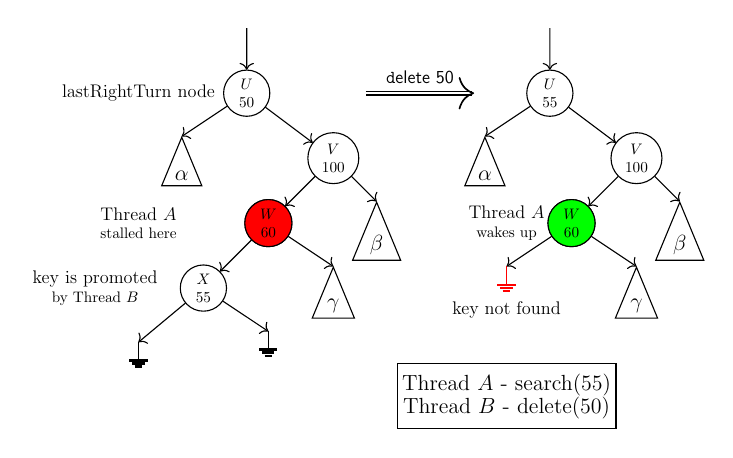
\begin{tikzpicture}[scale=0.55, transform shape,mylabel/.style={thin, draw=black, align=center, minimum width=0.3cm, minimum height=0.3cm,fill=white}]
		\newcommand\XA{0}
		\newcommand\YA{0}
		\node (x)		[treenode] 									at (-6,0)       							{$U$ \\ 50};
		\node (a)		[subtree] 									at (-7.5,-1)  								{\Large $\alpha$};
		\node (y0)	[treenode] 									at (-4,-1.5) 									{$V$ \\ 100};
		\node (y1)	[treenode]									at (-5.5,-3)									{$W$ \\ 60}; 
		\node (b)		[subtree] 									at (-3,-2.5)    							{\Large $\beta$};
		\node (y2)	[treenode]									at (-7,-4.5)									{$X$ \\ 55}; 
		\node (g)		[subtree] 									at (-4,-4)   									{\Large $\gamma$};
		\node (gnd)	[ground] 										at (-8.5,-5.75)								{}; 
		\node (o)		[ground] 										at (-5.5,-5.5)  							{};
		\node (x1) 	[] 													at (-8.5,0) 									{\large lastRightTurn node};
		\draw[->] (-6, 1.5) --  (x);
		\draw[->] (x) -- (y0);
		\draw[->] (x) -- (a.north);
		\draw[->] (y0) -- (y1);
		\draw[->] (y0) -- (b.north);
		\draw[->] (y1) -- (y2);
		\draw[->] (y1) -- (g.north);
		\draw[->] (y2) -- (gnd);
		\draw[->] (y2) -- (o);
		%% legend
		\node [thin, draw=black, align=center, minimum width=5cm, minimum height=1.5cm] at (0,-7) {\Large Thread $A$ - search(55) \\ \Large Thread $B$ - delete(50)};	
		\pause
		\node (y1)	[treenode, fill=red]		at (-5.5,-3)											{$W$ \\ 60}; 
		\node (y1l) [rectangle,align=center,minimum size=1cm] at (-8.5,-3) 		{\large Thread $A$ \\stalled here};
		\pause
		\node (y2l) [rectangle,align=center,minimum size=1cm] at(-9.5,-4.5) 	{\large key is promoted \\by Thread $B$};
		\pause
		\path[every node/.style={font=\sffamily\small}]
		(-3.25, 0) edge[->,semithick, double] node [above, outer sep=3pt] 		{\large \texttt delete 50} (-0.75, 0);

		\node (ix)	[treenode] 									at (1,0)       								{$U$ \\ 55};
		\node (ia)	[subtree] 									at (-0.5,-1)  								{\Large $\alpha$};
		\node (iy0)	[treenode] 									at (3,-1.5) 									{$V$ \\ 100};
		\node (iy1)	[treenode, fill=red]									at (1.5,-3)					{$W$ \\ 60}; 
		\node (ib)	[subtree] 									at (4,-2.5)    								{\Large $\beta$};
		\node (io)	[ground]										at (0,-4)											{}; 
		\node (ignd)[subtree] 									at (3,-4)   									{\Large $\gamma$};
    
    \draw[->] (1, 1.5) --  (ix);
    \draw[->] (ix) --  (iy0);
    \draw[->] (ix) --  (ia.north);
    \draw[->] (iy0) --  (iy1);
    \draw[->] (iy0) --  (ib.north);
    \draw[->] (iy1) --  (io);
    \draw[->] (iy1) --  (ignd.north);
		\pause
		\node (iy1)	[treenode, fill=green]									at (1.5,-3)					{$W$ \\ 60};
		\node (y12) [rectangle,align=center,minimum size=1cm] at (0,-3) 		{\large Thread $A$ \\wakes up};
		\pause
		\node (io)	[ground,color=red]										at (0,-4)											{}; 
		\node (y13) [rectangle,align=center,minimum size=1cm] at (0,-5) 		{\large key not found};
	\end{tikzpicture}


During seek we maintain two seek records: current and previous seek records. This is to prevent the scenario shown in Fig.~\ref{fig:issueInSeek}.

\end{comment}

\subsubsection{Helping}

To enable helping, as mentioned earlier, whenever traversing the tree to locate either a target key or a successor key, we keep track of the \emph{last two} edges encountered in the traversal. When a \CAS{} instruction fails, depending on the reason for failure, helping is either performed along the last edge or the second-to-last edge. 


\subsection{Formal Description}
A pseudo-code of our algorithm is given in \algosref{icdcn-data|structures}{icdcn-helping}.

\Algoref{icdcn-data|structures} describes the data structures used in our algorithm. Besides \textsf{Node}, three important data types in our algorithm are: \textsf{Edge}, \textsf{SeekRecord} and \textsf{StateRecord}. The data type \textsf{Edge} is a structure consisting of three fields: the two endpoints and the direction (left or right). The data type \textsf{SeekRecord} is a structure used to store the results of a tree traversal. The data type \textsf{StateRecord} is a structure used to store information about a delete operation (\emph{e.g.}, target edge, type,  current mode, etc.). Note that only objects of type \textsf{Node} are shared between processes; objects of all other types (\emph{e.g.}, \textsf{SeekRecord}, \textsf{StateRecord}) are \emph{local} to a process and not shared with other processes.

The pseudo-code of the seek function is described in \algoref{icdcn-seek}, which is used by all the operations. The pseudo-codes of the search, insert and delete operations are given in \algoref{icdcn-search}, \algoref{icdcn-insert} and \algoref{icdcn-delete}, respectively. A delete operation executes  function \Inject{} in \injection{} mode, functions \FindAndMarkSuccessor{} and \RemoveSuccessor{} in \discovery{} mode and function \Cleanup{} in \cleanup{} mode. Their pseudo-codes are given in \algoref{icdcn-inject}, \algoref{icdcn-findandmark}, \algoref{icdcn-remove} and \algoref{icdcn-cleanup}, respectively. The pseudo-codes for helper routines (used by multiple functions) are given in \algoref{icdcn-findSmallest}, \algoref{icdcn-markChildEdge} and \algoref{icdcn-helper|2}. Finally, the pseudo-codes of functions used to help other (conflicting) delete operations are given in \algoref{icdcn-helping}.

\section{Correctness Proof}
It is convenient to treat insert and delete operations that do not change the tree as search operations. We call a tree node \emph{active} if it is reachable from the root of the 
tree. We call a tree node  \emph{passive} if it was active earlier but is not active any more. Note that, before an active node is made passive by a delete operation, both its 
children edges are \emph{marked}. Also, a \CAS{} instruction performed on an edge (by either an insert operation or a delete operation as part of locking) is successful only if the edge is unmarked. As a result, clearly, if an insert operation completes successfully, then  its target node was active when its edge was modified to make the new node (containing the target key) a part of the tree. Likewise, if a delete operation completes successfully, then all the nodes involved in the operation (up to three nodes) were active when their edges were locked.

\subsection*{All Executions are Linearizable}

We show that an arbitrary execution of our algorithm is linearizable by specifying the \emph{linearization point} of each operation. Note that the linearization point of an operation is the point during its execution at which the operation appeared to have taken effect. Our algorithm supports three types of operations: search, insert and delete. We now specify the linearization point of each operation.

\begin{enumerate}[leftmargin=*]
\item \emph{Insert operation:} The operation is linearized at the point at which it performed the successful \CAS{} instruction that resulted in its target key becoming part of the tree.					
\item \emph{Delete operation:} There are two cases depending on whether the delete operation is simple or complex. If the operation is simple delete, then the operation is linearized at the point at which a successful write step was performed at the parent of the target node that resulted in the target node becoming passive. Otherwise, it is linearized at the point at which the original key of the target node was replaced with its successor key.   
\item \emph{Search operation:} There are two cases depending on whether the target node was active when the operation read the key stored in the node. If the target node was not active, then the operation is linearized at the point at which the target node became passive. Otherwise, it is linearized at the point at which the read step was performed.
\end{enumerate}

It can be easily verified that, for any execution of the algorithm, the sequence of operations obtained by ordering operations based on their linearization points is legal, \emph{i.e.}, all operations in the sequence satisfy their specification. 

Thus we have:
\begin{theorem}
Every execution of our algorithm is linearizable.
\end{theorem}
			 
\subsection*{All Executions are Deadlock-Free}	
We say that the system is in a \emph{quiescent state} if no modify operation completes hereafter. We say that the system is in a \emph{potent state} if it has one or more pending modify operations. Note that quiescence is a \emph{stable property}; once the system is in a quiescent state, it stays in a quiescent state. We show that our algorithm is deadlock-free by proving that a potent state is necessarily non-quiescent. 


Note that, in a quiescent state, no edges in the tree can be marked. This is because a delete operation marks edges only after it has successfully obtained all the locks, after which it is guaranteed to complete. This also implies that the tree cannot undergo any changes now because that would imply eventual completion of a modify operation. Thus, once a system has reached a quiescent state, all modify operation currently pending repeatedly alternate between seek and execution phases. We say that the system is in a \emph{strongly-quiescent state} if all pending modify operations started their most recent seek phase \emph{after} the system became quiescent. Note that, like quiescence, strong quiescence is also a stable property. Now, once the system has reached a strongly quiescent state, the following can be easily verified. First, for a given modify operation, every traversal of the tree in the seek phase returns the same target node. Second, for a given delete operation, the set of edges it needs to lock remains the same. 


Now, assume that the system eventually reaches a state that is both potent and quiescent. Clearly, from this state, the system will eventually reach a state that is potent and strongly-quiescent. Note that a delete operation in our algorithm locks edges in a \emph{top-down}, \emph{left-right} manner. As a result, there cannot be a ``cycle'' involving delete operations. If a delete operation continues to fail in the execution phase, then it is necessarily because it tried to acquire lock on an already locked edge. (Recall that the set of edges does not change any more and there are no marked edges in the tree.) We can construct a chain of operations such that each operation in the chain tried to lock an edge already locked by the next operation in the chain. Clearly, the length of the chain is bounded. This implies that the last operation in the chain is guaranteed to obtain all the locks and will eventually complete. This contradicts the fact that the system is in a quiescent state. 


Thus, we have:
\begin{theorem}
Every execution of our algorithm is deadlock-free.
\end{theorem}
\end{limitscope}
\section{Impact of local recovery}
\label{sec:experiments:localRecovery}
%\begin{limitscope}
%%%%% local recovery experiments macros - begin
\newcommand{\retries}{\emph {retries}}
\newcommand{\seekTime}{\emph {seek-time}}
\newcommand{\modifyTime}{\emph {modify-time}}
\newcommand{\seekLength}{\emph {seek-length}}
\newcommand{\estLatencyImpact}{\emph {latency-impact}}
\newcommand{\throughput}{\emph {throughput}}
\newcommand{\action}{modify}
%%%%% local recovery experiments macros - end

In this section we evaluate our local recovery technique. 

To show that our local recovery algorithm is sufficiently general, we implemented it for three different concurrent internal BSTs, namely those based on:
\begin{enumerate*}[label=(\roman*)]
\item the lock-free BST by Howley and Jones~\cite{HowJon:2012:SPAA}, denoted by \HJBST{},
\item the lock-based BST by Ramachandran and Mittal~\cite{RamMit:2015:PPoPP}, denoted by \CASTLE{} and
\item the RCU (Read-Copy-Update) lock-based BST by Arbel and Attiya~\cite{ArbAtt:2014:PODC}, denoted by \CITRUS{}.
\end{enumerate*}
These implementations were chosen so that we covered both lock-free and lock-based approaches. We choose two lock-based implementations as one is based on locking edges~\cite{RamMit:2015:PPoPP} and the other is based on locking nodes using RCU framework~\cite{ArbAtt:2014:PODC}.

\subsection*{Experimental Setup}
As local recovery is useful for high contention cases, we conducted our experiments on a single Intel Xeon Phi SE10P Coprocessor \footnote{http://www.intel.com/content/www/us/en/processors/xeon/xeon-phi-detail.html}
having 61 1.1 GHz cores with 4 hardware threads per core and 8GB of GDDR5 memory. With this machine we were able to experiment with up to 244 threads.

\subsection*{Key distribution}
Usually uniform key distribution (where all keys have same frequency of occurrence) have been used to evaluate concurrent BSTs. But in many of the real world workloads, keys have skewed distribution~\cite{ClaSha+:2009:SIAM} where some keys are more popular than others. Zipfian distribution, a type of power-law distribution simulates this behaviour~\cite{BreCao+:1999:INFOCOM,FalJag:1992:VLDB,GraSun+:1994:SIGMOD}. It is characterized by a parameter $\alpha$ which usually lies between 0.5 and 1~\cite{BreCao+:1999:INFOCOM,AdaHub:2002:GLOTTMET}. In our experiments we used both uniform and Zipfian distributions to evaluate the local recovery algorithm.

\subsection*{Simulation results}
\Tabref{localRecovery-perf-numbers} summarizes the performance gap (with respect to system throughput) between the base algorithm and its extension using local recovery for uniform and Zipfian distributions. 
\begin{table}[tp]
\centering
\caption{Effect of local recovery on system throughput. Positive number indicates a gain while a negative number indicates a drop.}
\label{tab:perf-numbers}
\begin{tabular}{|c|c|c|}
\hline
{\bf Algorithm}  & {\bf \begin{tabular}[c]{@{}c@{}}Uniform\\ (max\%, min\%)\end{tabular}} & {\bf \begin{tabular}[c]{@{}c@{}}Zipfian\\ (max\%, min\%)\end{tabular}} \\ \hline
{\bf \CASTLE{}} & (6, -7)                                                            & (23, -11)                                                            \\ \hline
{\bf \CITRUS{}} & (23, -11)                                                            & (20, -13)                                                             \\ \hline
{\bf \HJBST{}}  & (9, -6)                                                            & (49, -6)                                                           \\ \hline
\end{tabular}
\end{table}

To better understand the effect of local recovery, we also measure several metrics defined in \tabref{metrics-definition}.
\begin{table}
\centering
\caption{Performance metrics used to evaluate the effect of local recovery.}
\label{tab:metrics-definition}
\begin{tabular}{|l|>{}m{0.7\linewidth}|}
\hline
{\bf Metric}					& {\bf Description} 		\\ \hline
{\retries} 				& { fraction of restarts for an operation}      					\\ \hline
{\seekTime}  					& {total time an operation spends on tree traversal including all restarts as well as stack processing time (in $\mu$s)}  \\ \hline
{\modifyTime}  					& {total time an operation spends on \action{} phase (in $\mu$s)}      					\\ \hline
{\seekLength} 				& {number of nodes traversed in the tree by an operation}      					\\ \hline
{\estLatencyImpact}		& {a rough approximation of the amount of clock cycles devoted to each L1 cache miss (a measure of cache performance)~\cite{JefRei:2013:Book}}      					\\ \hline
\end{tabular}                
\end{table}
\Figsref{localRecovery-throughput-uniform}{metrics-uniform} show the impact of local recovery on throughput and various metrics for uniform distribution. We see that the performance gain is marginal and, in many cases, is actually slightly worse due to the overhead of stack maintenance. This is not surprising because, for small trees, even though contention is higher, seek time is small to begin with and any benefit of local recovery is nullified by additional overhead of stack maintenance. For larger trees, even though seek time is larger, contention is low as key accesses are spread evenly.
% Style to select only points from #1 to #2 (inclusive)
\pgfplotsset
{
	select coords between index/.style 2 args=
	{
    x filter/.code=
		{
        \ifnum\coordindex<#1\def\pgfmathresult{}\fi
        \ifnum\coordindex>#2\def\pgfmathresult{}\fi
    }
	}
}
\begin{figure}
\centering
\nextwithlateexternal% < added
\begin{tikzpicture}
	\begin{groupplot}[group style={group size= 4 by 3},height=5.25cm,width=4.5cm,max space between ticks=20,minor tick num=1,tick label style={font=\scriptsize}]
		\nextgroupplot[title={\scriptsize 2K keys},ylabel={\scriptsize Read-Dominated},y label style={at={(0.15,0.5)}},xtick={1,61,122,183,244},mark size=1.5pt]
				\addplot[black, densely dashed,mark=square] [select coords between index={0}{8}] 		table[x=NumOfThreads,y=citrus-MOPS,col sep=space]	 	{Data/localRecovery/mic/threadSweep-uniform.csv}; 	\label{plots:CITRUS:mopsU}
				\addplot[red,densely dashed,mark=triangle*] [select coords between index={0}{8}] 		table[x=NumOfThreads,y=howley-MOPS,col sep=space]	 	{Data/localRecovery/mic/threadSweep-uniform.csv}; 	\label{plots:HOWLEY:mopsU}
				%\addplot[blue,densely dashed,mark=asterisk][select coords between index={0}{8}] 		table[x=NumOfThreads,y=icdcn-MOPS,col sep=space] 	 	{Data/localRecovery/mic/threadSweep-uniform.csv};  	\label{plots:ICDCN:mopsU}
				\addplot[green, densely dashed,mark=o] 		 	[select coords between index={0}{8}] 		table[x=NumOfThreads,y=castle-MOPS,col sep=space]	 	{Data/localRecovery/mic/threadSweep-uniform.csv}; 	\label{plots:CASTLE:mopsU}
				\addplot[black, semithick,mark=square] 	  	[select coords between index={0}{8}] 		table[x=NumOfThreads,y=citrusL-MOPS,col sep=space]	{Data/localRecovery/mic/threadSweep-uniform.csv}; 	\label{plots:CITRUSL:mopsU}
				\addplot[red,semithick,mark=triangle*] 			[select coords between index={0}{8}] 		table[x=NumOfThreads,y=howleyL-MOPS,col sep=space]	{Data/localRecovery/mic/threadSweep-uniform.csv}; 	\label{plots:HOWLEYL:mopsU}
				%\addplot[blue,semithick,mark=asterisk] 		[select coords between index={0}{8}] 		table[x=NumOfThreads,y=icdcnL-MOPS,col sep=space] 	{Data/localRecovery/mic/threadSweep-uniform.csv};  	\label{plots:ICDCNL:mopsU}
				\addplot[green, semithick,mark=o] 					[select coords between index={0}{8}] 		table[x=NumOfThreads,y=castleL-MOPS,col sep=space]	{Data/localRecovery/mic/threadSweep-uniform.csv}; 	\label{plots:CASTLEL:mopsU}
				\coordinate (top) at (rel axis cs:0,1);% coordinate at top of the first plot	
		\nextgroupplot[title={\scriptsize 20K keys},xtick={1,61,122,183,244},mark size=1.5pt]	
				\addplot[black, densely dashed,mark=square] [select coords between index={9}{17}] 	table[x=NumOfThreads,y=citrus-MOPS,col sep=space] 	{Data/localRecovery/mic/threadSweep-uniform.csv};  
				\addplot[red,densely dashed,mark=triangle*] [select coords between index={9}{17}] 	table[x=NumOfThreads,y=howley-MOPS,col sep=space] 	{Data/localRecovery/mic/threadSweep-uniform.csv};  
				%\addplot[blue,densely dashed,mark=asterisk][select coords between index={9}{17}] 	table[x=NumOfThreads,y=icdcn-MOPS,col sep=space]  	{Data/localRecovery/mic/threadSweep-uniform.csv};  
				\addplot[green, densely dashed,mark=o] 			[select coords between index={9}{17}] 	table[x=NumOfThreads,y=castle-MOPS,col sep=space] 	{Data/localRecovery/mic/threadSweep-uniform.csv}; 
				\addplot[black, semithick,mark=square] 			[select coords between index={9}{17}] 	table[x=NumOfThreads,y=citrusL-MOPS,col sep=space] 	{Data/localRecovery/mic/threadSweep-uniform.csv};
				\addplot[red,semithick,mark=triangle*] 			[select coords between index={9}{17}] 	table[x=NumOfThreads,y=howleyL-MOPS,col sep=space] 	{Data/localRecovery/mic/threadSweep-uniform.csv};
				%\addplot[blue,semithick,mark=asterisk] 		[select coords between index={9}{17}] 	table[x=NumOfThreads,y=icdcnL-MOPS,col sep=space]  	{Data/localRecovery/mic/threadSweep-uniform.csv}; 
				\addplot[green, semithick,mark=o] 					[select coords between index={9}{17}] 	table[x=NumOfThreads,y=castleL-MOPS,col sep=space] 	{Data/localRecovery/mic/threadSweep-uniform.csv};
		\nextgroupplot[title={\scriptsize 200K keys},xtick={1,61,122,183,244},mark size=1.5pt]
				\addplot[black, densely dashed,mark=square] [select coords between index={18}{26}] 	table[x=NumOfThreads,y=citrus-MOPS,col sep=space] 	{Data/localRecovery/mic/threadSweep-uniform.csv};
				\addplot[red,densely dashed,mark=triangle*] [select coords between index={18}{26}] 	table[x=NumOfThreads,y=howley-MOPS,col sep=space] 	{Data/localRecovery/mic/threadSweep-uniform.csv};
				%\addplot[blue,densely dashed,mark=asterisk][select coords between index={18}{26}] 	table[x=NumOfThreads,y=icdcn-MOPS,col sep=space]  	{Data/localRecovery/mic/threadSweep-uniform.csv};
				\addplot[green, densely dashed,mark=o] 			[select coords between index={18}{26}] 	table[x=NumOfThreads,y=castle-MOPS,col sep=space] 	{Data/localRecovery/mic/threadSweep-uniform.csv};
				\addplot[black, semithick,mark=square] 			[select coords between index={18}{26}] 	table[x=NumOfThreads,y=citrusL-MOPS,col sep=space] 	{Data/localRecovery/mic/threadSweep-uniform.csv};
				\addplot[red,semithick,mark=triangle*] 			[select coords between index={18}{26}] 	table[x=NumOfThreads,y=howleyL-MOPS,col sep=space] 	{Data/localRecovery/mic/threadSweep-uniform.csv};
				%\addplot[blue,semithick,mark=asterisk] 		[select coords between index={18}{26}] 	table[x=NumOfThreads,y=icdcnL-MOPS,col sep=space]  	{Data/localRecovery/mic/threadSweep-uniform.csv}; 
				\addplot[green, semithick,mark=o] 					[select coords between index={18}{26}] 	table[x=NumOfThreads,y=castleL-MOPS,col sep=space] 	{Data/localRecovery/mic/threadSweep-uniform.csv};
		\nextgroupplot[title={\scriptsize 2M keys},xtick={1,61,122,183,244},mark size=1.5pt]	
				\addplot[black, densely dashed,mark=square] [select coords between index={27}{35}] 	table[x=NumOfThreads,y=citrus-MOPS,col sep=space] 	{Data/localRecovery/mic/threadSweep-uniform.csv}; 
				\addplot[red,densely dashed,mark=triangle*] [select coords between index={27}{35}] 	table[x=NumOfThreads,y=howley-MOPS,col sep=space] 	{Data/localRecovery/mic/threadSweep-uniform.csv};
				%\addplot[blue,densely dashed,mark=asterisk][select coords between index={27}{35}] 	table[x=NumOfThreads,y=icdcn-MOPS,col sep=space]  	{Data/localRecovery/mic/threadSweep-uniform.csv};
				\addplot[green, densely dashed,mark=o] 			[select coords between index={27}{35}] 	table[x=NumOfThreads,y=castle-MOPS,col sep=space] 	{Data/localRecovery/mic/threadSweep-uniform.csv};
				\addplot[black, semithick,mark=square] 			[select coords between index={27}{35}] 	table[x=NumOfThreads,y=citrusL-MOPS,col sep=space] 	{Data/localRecovery/mic/threadSweep-uniform.csv};
				\addplot[red,semithick,mark=triangle*] 			[select coords between index={27}{35}] 	table[x=NumOfThreads,y=howleyL-MOPS,col sep=space] 	{Data/localRecovery/mic/threadSweep-uniform.csv};
				%\addplot[blue,semithick,mark=asterisk] 		[select coords between index={27}{35}] 	table[x=NumOfThreads,y=icdcnL-MOPS,col sep=space]  	{Data/localRecovery/mic/threadSweep-uniform.csv}; 
				\addplot[green, semithick,mark=o] 					[select coords between index={27}{35}] 	table[x=NumOfThreads,y=castleL-MOPS,col sep=space] 	{Data/localRecovery/mic/threadSweep-uniform.csv};
		\nextgroupplot[ylabel={\scriptsize Mixed},y label style={at={(0.15,0.5)}},xtick={1,61,122,183,244},mark size=1.5pt]		
				\addplot[black, densely dashed,mark=square] [select coords between index={36}{44}] 	table[x=NumOfThreads,y=citrus-MOPS,col sep=space] 	{Data/localRecovery/mic/threadSweep-uniform.csv}; 
				\addplot[red,densely dashed,mark=triangle*] [select coords between index={36}{44}] 	table[x=NumOfThreads,y=howley-MOPS,col sep=space] 	{Data/localRecovery/mic/threadSweep-uniform.csv};
				%\addplot[blue,densely dashed,mark=asterisk][select coords between index={36}{44}] 	table[x=NumOfThreads,y=icdcn-MOPS,col sep=space]  	{Data/localRecovery/mic/threadSweep-uniform.csv};
				\addplot[green, densely dashed,mark=o] 			[select coords between index={36}{44}] 	table[x=NumOfThreads,y=castle-MOPS,col sep=space] 	{Data/localRecovery/mic/threadSweep-uniform.csv};
				\addplot[black, semithick,mark=square] 			[select coords between index={36}{44}] 	table[x=NumOfThreads,y=citrusL-MOPS,col sep=space] 	{Data/localRecovery/mic/threadSweep-uniform.csv};
				\addplot[red,semithick,mark=triangle*] 			[select coords between index={36}{44}] 	table[x=NumOfThreads,y=howleyL-MOPS,col sep=space] 	{Data/localRecovery/mic/threadSweep-uniform.csv};
				%\addplot[blue,semithick,mark=asterisk] 		[select coords between index={36}{44}] 	table[x=NumOfThreads,y=icdcnL-MOPS,col sep=space]  	{Data/localRecovery/mic/threadSweep-uniform.csv}; 
				\addplot[green, semithick,mark=o] 					[select coords between index={36}{44}] 	table[x=NumOfThreads,y=castleL-MOPS,col sep=space] 	{Data/localRecovery/mic/threadSweep-uniform.csv};
		\nextgroupplot[xtick={1,61,122,183,244},mark size=1.5pt]		
				\addplot[black, densely dashed,mark=square] [select coords between index={45}{53}] 	table[x=NumOfThreads,y=citrus-MOPS,col sep=space] 	{Data/localRecovery/mic/threadSweep-uniform.csv}; 
				\addplot[red,densely dashed,mark=triangle*] [select coords between index={45}{53}] 	table[x=NumOfThreads,y=howley-MOPS,col sep=space] 	{Data/localRecovery/mic/threadSweep-uniform.csv};
				%\addplot[blue,densely dashed,mark=asterisk][select coords between index={45}{53}] 	table[x=NumOfThreads,y=icdcn-MOPS,col sep=space]  	{Data/localRecovery/mic/threadSweep-uniform.csv};
				\addplot[green, densely dashed,mark=o] 			[select coords between index={45}{53}] 	table[x=NumOfThreads,y=castle-MOPS,col sep=space] 	{Data/localRecovery/mic/threadSweep-uniform.csv};
				\addplot[black, semithick,mark=square] 			[select coords between index={45}{53}] 	table[x=NumOfThreads,y=citrusL-MOPS,col sep=space] 	{Data/localRecovery/mic/threadSweep-uniform.csv};
				\addplot[red,semithick,mark=triangle*] 			[select coords between index={45}{53}] 	table[x=NumOfThreads,y=howleyL-MOPS,col sep=space] 	{Data/localRecovery/mic/threadSweep-uniform.csv};
				%\addplot[blue,semithick,mark=asterisk] 		[select coords between index={45}{53}] 	table[x=NumOfThreads,y=icdcnL-MOPS,col sep=space]  	{Data/localRecovery/mic/threadSweep-uniform.csv}; 
				\addplot[green, semithick,mark=o] 					[select coords between index={45}{53}] 	table[x=NumOfThreads,y=castleL-MOPS,col sep=space] 	{Data/localRecovery/mic/threadSweep-uniform.csv};
		\nextgroupplot[xtick={1,61,122,183,244},mark size=1.5pt]		
				\addplot[black, densely dashed,mark=square] [select coords between index={54}{62}] 	table[x=NumOfThreads,y=citrus-MOPS,col sep=space] 	{Data/localRecovery/mic/threadSweep-uniform.csv}; 
				\addplot[red,densely dashed,mark=triangle*] [select coords between index={54}{62}] 	table[x=NumOfThreads,y=howley-MOPS,col sep=space] 	{Data/localRecovery/mic/threadSweep-uniform.csv};
				%\addplot[blue,densely dashed,mark=asterisk][select coords between index={54}{62}] 	table[x=NumOfThreads,y=icdcn-MOPS,col sep=space]  	{Data/localRecovery/mic/threadSweep-uniform.csv};
				\addplot[green, densely dashed,mark=o] 			[select coords between index={54}{62}] 	table[x=NumOfThreads,y=castle-MOPS,col sep=space] 	{Data/localRecovery/mic/threadSweep-uniform.csv};	
				\addplot[black, semithick,mark=square] 			[select coords between index={54}{62}] 	table[x=NumOfThreads,y=citrusL-MOPS,col sep=space] 	{Data/localRecovery/mic/threadSweep-uniform.csv};
				\addplot[red,semithick,mark=triangle*] 			[select coords between index={54}{62}] 	table[x=NumOfThreads,y=howleyL-MOPS,col sep=space] 	{Data/localRecovery/mic/threadSweep-uniform.csv};
				%\addplot[blue,semithick,mark=asterisk] 		[select coords between index={54}{62}] 	table[x=NumOfThreads,y=icdcnL-MOPS,col sep=space]  	{Data/localRecovery/mic/threadSweep-uniform.csv}; 
				\addplot[green, semithick,mark=o] 					[select coords between index={54}{62}] 	table[x=NumOfThreads,y=castleL-MOPS,col sep=space] 	{Data/localRecovery/mic/threadSweep-uniform.csv};
		\nextgroupplot[xtick={1,61,122,183,244},mark size=1.5pt]		
				\addplot[black, densely dashed,mark=square] [select coords between index={63}{71}] 	table[x=NumOfThreads,y=citrus-MOPS,col sep=space] 	{Data/localRecovery/mic/threadSweep-uniform.csv}; 
				\addplot[red,densely dashed,mark=triangle*] [select coords between index={63}{71}] 	table[x=NumOfThreads,y=howley-MOPS,col sep=space] 	{Data/localRecovery/mic/threadSweep-uniform.csv};
				%\addplot[blue,densely dashed,mark=asterisk][select coords between index={63}{71}] 	table[x=NumOfThreads,y=icdcn-MOPS,col sep=space]  	{Data/localRecovery/mic/threadSweep-uniform.csv};
				\addplot[green, densely dashed,mark=o] 			[select coords between index={63}{71}] 	table[x=NumOfThreads,y=castle-MOPS,col sep=space] 	{Data/localRecovery/mic/threadSweep-uniform.csv};
				\addplot[black, semithick,mark=square] 			[select coords between index={63}{71}] 	table[x=NumOfThreads,y=citrusL-MOPS,col sep=space] 	{Data/localRecovery/mic/threadSweep-uniform.csv};
				\addplot[red,semithick,mark=triangle*] 			[select coords between index={63}{71}] 	table[x=NumOfThreads,y=howleyL-MOPS,col sep=space] 	{Data/localRecovery/mic/threadSweep-uniform.csv};
				%\addplot[blue,semithick,mark=asterisk] 		[select coords between index={63}{71}] 	table[x=NumOfThreads,y=icdcnL-MOPS,col sep=space]  	{Data/localRecovery/mic/threadSweep-uniform.csv}; 
				\addplot[green, semithick,mark=o] 					[select coords between index={63}{71}] 	table[x=NumOfThreads,y=castleL-MOPS,col sep=space] 	{Data/localRecovery/mic/threadSweep-uniform.csv};				
		\nextgroupplot[xlabel={\scriptsize Number of Threads},ylabel={\scriptsize Write-Dominated},y label style={at={(0.15,0.5)}},xtick={1,61,122,183,	244},mark size=1.5pt]
				\addplot[black, densely dashed,mark=square] [select coords between index={72}{80}] 	table[x=NumOfThreads,y=citrus-MOPS,col sep=space] 	{Data/localRecovery/mic/threadSweep-uniform.csv};    
				\addplot[red,densely dashed,mark=triangle*] [select coords between index={72}{80}] 	table[x=NumOfThreads,y=howley-MOPS,col sep=space] 	{Data/localRecovery/mic/threadSweep-uniform.csv};    
				%\addplot[blue,densely dashed,mark=asterisk][select coords between index={72}{80}] 	table[x=NumOfThreads,y=icdcn-MOPS,col sep=space]  	{Data/localRecovery/mic/threadSweep-uniform.csv};     
				\addplot[green, densely dashed,mark=o] 			[select coords between index={72}{80}] 	table[x=NumOfThreads,y=castle-MOPS,col sep=space] 	{Data/localRecovery/mic/threadSweep-uniform.csv};	   
				\addplot[black, semithick,mark=square] 			[select coords between index={72}{80}] 	table[x=NumOfThreads,y=citrusL-MOPS,col sep=space] 	{Data/localRecovery/mic/threadSweep-uniform.csv}; 
				\addplot[red,semithick,mark=triangle*] 			[select coords between index={72}{80}] 	table[x=NumOfThreads,y=howleyL-MOPS,col sep=space] 	{Data/localRecovery/mic/threadSweep-uniform.csv};   
				%\addplot[blue,semithick,mark=asterisk] 		[select coords between index={72}{80}] 	table[x=NumOfThreads,y=icdcnL-MOPS,col sep=space]  	{Data/localRecovery/mic/threadSweep-uniform.csv};    
				\addplot[green, semithick,mark=o] 					[select coords between index={72}{80}] 	table[x=NumOfThreads,y=castleL-MOPS,col sep=space] 	{Data/localRecovery/mic/threadSweep-uniform.csv};	
		\nextgroupplot[xlabel={\scriptsize Number of Threads},xtick={1,61,122,183,244},mark size=1.5pt]	
				\addplot[black, densely dashed,mark=square] [select coords between index={81}{89}] 	table[x=NumOfThreads,y=citrus-MOPS,col sep=space] 	{Data/localRecovery/mic/threadSweep-uniform.csv}; 
				\addplot[red,densely dashed,mark=triangle*] [select coords between index={81}{89}] 	table[x=NumOfThreads,y=howley-MOPS,col sep=space] 	{Data/localRecovery/mic/threadSweep-uniform.csv};
				%\addplot[blue,densely dashed,mark=asterisk][select coords between index={81}{89}] 	table[x=NumOfThreads,y=icdcn-MOPS,col sep=space]  	{Data/localRecovery/mic/threadSweep-uniform.csv};
				\addplot[green, densely dashed,mark=o] 			[select coords between index={81}{89}] 	table[x=NumOfThreads,y=castle-MOPS,col sep=space] 	{Data/localRecovery/mic/threadSweep-uniform.csv};	
				\addplot[black, semithick,mark=square] 			[select coords between index={81}{89}] 	table[x=NumOfThreads,y=citrusL-MOPS,col sep=space] 	{Data/localRecovery/mic/threadSweep-uniform.csv};
				\addplot[red,semithick,mark=triangle*] 			[select coords between index={81}{89}] 	table[x=NumOfThreads,y=howleyL-MOPS,col sep=space] 	{Data/localRecovery/mic/threadSweep-uniform.csv};
				%\addplot[blue,semithick,mark=asterisk] 		[select coords between index={81}{89}] 	table[x=NumOfThreads,y=icdcnL-MOPS,col sep=space]  	{Data/localRecovery/mic/threadSweep-uniform.csv}; 
				\addplot[green, semithick,mark=o] 					[select coords between index={81}{89}] 	table[x=NumOfThreads,y=castleL-MOPS,col sep=space] 	{Data/localRecovery/mic/threadSweep-uniform.csv};
		\nextgroupplot[xlabel={\scriptsize Number of Threads},xtick={1,61,122,183,244},mark size=1.5pt]	
				\addplot[black, densely dashed,mark=square] [select coords between index={90}{98}] 	table[x=NumOfThreads,y=citrus-MOPS,col sep=space] 	{Data/localRecovery/mic/threadSweep-uniform.csv}; 
				\addplot[red,densely dashed,mark=triangle*] [select coords between index={90}{98}] 	table[x=NumOfThreads,y=howley-MOPS,col sep=space] 	{Data/localRecovery/mic/threadSweep-uniform.csv};
				%\addplot[blue,densely dashed,mark=asterisk][select coords between index={90}{98}] 	table[x=NumOfThreads,y=icdcn-MOPS,col sep=space]  	{Data/localRecovery/mic/threadSweep-uniform.csv};
				\addplot[green, densely dashed,mark=o] 			[select coords between index={90}{98}] 	table[x=NumOfThreads,y=castle-MOPS,col sep=space] 	{Data/localRecovery/mic/threadSweep-uniform.csv};	
				\addplot[black, semithick,mark=square] 			[select coords between index={90}{98}] 	table[x=NumOfThreads,y=citrusL-MOPS,col sep=space] 	{Data/localRecovery/mic/threadSweep-uniform.csv};
				\addplot[red,semithick,mark=triangle*] 			[select coords between index={90}{98}] 	table[x=NumOfThreads,y=howleyL-MOPS,col sep=space] 	{Data/localRecovery/mic/threadSweep-uniform.csv};
				%\addplot[blue,semithick,mark=asterisk] 		[select coords between index={90}{98}] 	table[x=NumOfThreads,y=icdcnL-MOPS,col sep=space]  	{Data/localRecovery/mic/threadSweep-uniform.csv}; 
				\addplot[green, semithick,mark=o] 					[select coords between index={90}{98}] 	table[x=NumOfThreads,y=castleL-MOPS,col sep=space] 	{Data/localRecovery/mic/threadSweep-uniform.csv};
		\nextgroupplot[xlabel={\scriptsize Number of Threads},xtick={1,61,122,183,244},mark size=1.5pt]	
				\addplot[black, densely dashed,mark=square] [select coords between index={99}{107}]	table[x=NumOfThreads,y=citrus-MOPS,col sep=space] 	{Data/localRecovery/mic/threadSweep-uniform.csv}; 
				\addplot[red,densely dashed,mark=triangle*] [select coords between index={99}{107}]	table[x=NumOfThreads,y=howley-MOPS,col sep=space] 	{Data/localRecovery/mic/threadSweep-uniform.csv};
				%\addplot[blue,densely dashed,mark=asterisk][select coords between index={99}{107}]	table[x=NumOfThreads,y=icdcn-MOPS,col sep=space]  	{Data/localRecovery/mic/threadSweep-uniform.csv};
				\addplot[green, densely dashed,mark=o] 			[select coords between index={99}{107}]	table[x=NumOfThreads,y=castle-MOPS,col sep=space] 	{Data/localRecovery/mic/threadSweep-uniform.csv};		
				\addplot[black, semithick,mark=square] 			[select coords between index={99}{107}]	table[x=NumOfThreads,y=citrusL-MOPS,col sep=space] 	{Data/localRecovery/mic/threadSweep-uniform.csv};
				\addplot[red,semithick,mark=triangle*] 			[select coords between index={99}{107}]	table[x=NumOfThreads,y=howleyL-MOPS,col sep=space] 	{Data/localRecovery/mic/threadSweep-uniform.csv};
				%\addplot[blue,semithick,mark=asterisk] 		[select coords between index={99}{107}]	table[x=NumOfThreads,y=icdcnL-MOPS,col sep=space]  	{Data/localRecovery/mic/threadSweep-uniform.csv}; 
				\addplot[green, semithick,mark=o] 					[select coords between index={99}{107}]	table[x=NumOfThreads,y=castleL-MOPS,col sep=space] 	{Data/localRecovery/mic/threadSweep-uniform.csv};				
				\coordinate (bot) at (rel axis cs:1,0);% coordinate at bottom of the last plot
\end{groupplot}
	\path (top-|current bounding box.west)-- node[anchor=south,rotate=90] {\scriptsize system throughput} (bot-|current bounding box.west);
	\path (top|-current bounding box.north)-- coordinate(legendpos) (bot|-current bounding box.north);
	\matrix[matrix of nodes, anchor=south, draw, inner sep=0.2em, draw] at ([yshift=1ex]legendpos)
  {
    \ref{plots:HOWLEY:mopsU}& 	\HJBST{} 				& [5pt]
    %\ref{plots:ICDCN:mopsU}& 	\ICDCN{} 				& [5pt]
    \ref{plots:CITRUS:mopsU}& 	\CITRUS{} 			& [5pt]
		\ref{plots:CASTLE:mopsU}& 	\CASTLE{} 			\\
		\ref{plots:HOWLEYL:mopsU}& 	\HJBST{} (LR)		& [5pt]
    %\ref{plots:ICDCNL:mopsU}& 	\ICDCN{} (LR)		& [5pt]
    \ref{plots:CITRUSL:mopsU}& 	\CITRUS{} (LR)	& [5pt]
		\ref{plots:CASTLEL:mopsU}& 	\CASTLE{}	(LR)	\\
	};
\end{tikzpicture}
\caption[Impact of local recovery on throughput - uniform distribution]{Comparison of throughput of different concurrent BST implementations with (solid lines) and without (dotted lines) local recovery for uniform distribution. Each row represents a workload type. Each column represents a key space range. Higher is better.}
\label{fig:localRecovery-throughput-uniform}
\end{figure}
% Style to select only points from #1 to #2 (inclusive)
\pgfplotsset{
  select row/.style={
    x filter/.code={\ifnum\coordindex=#1\else\def\pgfmathresult{}\fi}
  },
}

\definecolor{colorbrewer1}{RGB}{166,206,227}
\definecolor{colorbrewer2}{RGB}{31,120,180}
\definecolor{colorbrewer3}{RGB}{178,223,138}
\definecolor{colorbrewer4}{RGB}{51,160,44}
\definecolor{colorbrewer5}{RGB}{251,154,153}
\definecolor{colorbrewer6}{RGB}{227,26,28}
\definecolor{colorbrewer7}{RGB}{253,191,111}
\definecolor{colorbrewer8}{RGB}{255,127,0}
\definecolor{colorbrewer9}{RGB}{202,178,214}
\definecolor{colorbrewer10}{RGB}{106,61,154}
\definecolor{colorbrewer11}{RGB}{222,179,155}
\definecolor{colorbrewer12}{RGB}{177,89,40}
			
\pgfplotscreateplotcyclelist{paired}{
{draw=colorbrewer1 ,pattern color=colorbrewer1 ,pattern=horizontal lines},
{draw=colorbrewer2 ,pattern color=colorbrewer2 ,pattern=horizontal lines},
{draw=colorbrewer3 ,pattern color=colorbrewer3 ,pattern=vertical lines},
{draw=colorbrewer4 ,pattern color=colorbrewer4 ,pattern=vertical lines},
{draw=colorbrewer5 ,pattern color=colorbrewer5 ,pattern=north east lines},
{draw=colorbrewer6 ,pattern color=colorbrewer6 ,pattern=north east lines},
{draw=colorbrewer7 ,pattern color=colorbrewer7 ,pattern=north west lines},
{draw=colorbrewer8 ,pattern color=colorbrewer8 ,pattern=north west lines},
{draw=colorbrewer9 ,pattern color=colorbrewer9 ,pattern=grid},
{draw=colorbrewer10,pattern color=colorbrewer10,pattern=grid},
{draw=colorbrewer11,pattern color=colorbrewer11,pattern=crosshatch},
{draw=colorbrewer12,pattern color=colorbrewer12,pattern=crosshatch}}
			
\def\twinplot#1#2{
  \pgfplotsforeachungrouped \row in {0,...,5}{
      \edef\justplotit{
        \noexpand\addplot+[bar shift=(-0.5)*\pgfplotbarwidth]
          table [x=metric, select row=\row, y=#1] {#2};}
      \justplotit
			\edef\justplotit{
        \noexpand\addplot+[bar shift=(0.5)*\pgfplotbarwidth]
          table [x=metric, select row=\row, y=#1L] {#2};}
      \justplotit
  }
}

\begin{figure}
\centering
\nextwithlateexternal% < added
\begin{tikzpicture}
\begin{groupplot}
	[
    group style={group size= 3 by 6,xticklabels at=edge bottom},
    height=3.5cm,
    width=5cm,
    ybar=1pt,
    tick label style={font=\scriptsize},
    x tick label style={rotate=45,anchor=east},
    symbolic x coords={retries,seek-time,modify-time,seek-length,throughput},
    ylabel style={align=center},
		cycle list name=paired,
    max space between ticks=15,
		ymin=0
  ]
	\pgfkeys{/pgf/bar width=5.5pt}
	
	\nextgroupplot[title=\CASTLE,ylabel={\scriptsize 2K}] \twinplot{castle}{Data/localRecovery/mic/scaled/uniform/2k-90-9-1.csv}
	%\nextgroupplot[title=\ICDCN] 						\twinplot{icdcn}{Data/localRecovery/mic/scaled/uniform/2k-90-9-1.csv}
	\nextgroupplot[title=\CITRUS] 						\twinplot{citrus}{Data/localRecovery/mic/scaled/uniform/2k-90-9-1.csv}
	\nextgroupplot[title=\HJBST] 							\twinplot{howley}{Data/localRecovery/mic/scaled/uniform/2k-90-9-1.csv}
	\coordinate (mtop0) at (rel axis cs:0,1);% coordinate at top of the first plot
		
	\nextgroupplot[ylabel={\scriptsize 200K}]							\twinplot{castle}{Data/localRecovery/mic/scaled/uniform/200k-90-9-1.csv}
	%\nextgroupplot														\twinplot{icdcn}{Data/localRecovery/mic/scaled/uniform/200k-90-9-1.csv}
	\nextgroupplot														\twinplot{citrus}{Data/localRecovery/mic/scaled/uniform/200k-90-9-1.csv}
	\nextgroupplot														\twinplot{howley}{Data/localRecovery/mic/scaled/uniform/200k-90-9-1.csv}
	\coordinate (mbot0) at (rel axis cs:1,0);% coordinate at bottom of the last plot
	
	\nextgroupplot[ylabel={\scriptsize 2K}] 							\twinplot{castle}{Data/localRecovery/mic/scaled/uniform/2k-70-20-10.csv}
	%\nextgroupplot														\twinplot{icdcn}{Data/localRecovery/mic/scaled/uniform/2k-70-20-10.csv}
	\nextgroupplot						  							\twinplot{citrus}{Data/localRecovery/mic/scaled/uniform/2k-70-20-10.csv}
	\nextgroupplot						  							\twinplot{howley}{Data/localRecovery/mic/scaled/uniform/2k-70-20-10.csv}
	\coordinate (mtop) at (rel axis cs:0,1);% coordinate at top of the first plot
		
	\nextgroupplot[ylabel={\scriptsize 200K}]							\twinplot{castle}{Data/localRecovery/mic/scaled/uniform/200k-70-20-10.csv}
	%\nextgroupplot														\twinplot{icdcn}{Data/localRecovery/mic/scaled/uniform/200k-70-20-10.csv}
	\nextgroupplot														\twinplot{citrus}{Data/localRecovery/mic/scaled/uniform/200k-70-20-10.csv}
	\nextgroupplot														\twinplot{howley}{Data/localRecovery/mic/scaled/uniform/200k-70-20-10.csv}
	\coordinate (mbot) at (rel axis cs:1,0);% coordinate at bottom of the last plot
	
	\nextgroupplot[ylabel={\scriptsize 2K}]								\twinplot{castle}{Data/localRecovery/mic/scaled/uniform/2k-0-50-50.csv}
	%\nextgroupplot														\twinplot{icdcn}{Data/localRecovery/mic/scaled/uniform/2k-0-50-50.csv}
	\nextgroupplot														\twinplot{citrus}{Data/localRecovery/mic/scaled/uniform/2k-0-50-50.csv}
	\nextgroupplot														\twinplot{howley}{Data/localRecovery/mic/scaled/uniform/2k-0-50-50.csv}
	\coordinate (wtop) at (rel axis cs:0,1);% coordinate at top of the first plot
	
	\nextgroupplot[ylabel={\scriptsize 200K}]							\twinplot{castle}{Data/localRecovery/mic/scaled/uniform/200k-0-50-50.csv}
	%\nextgroupplot														\twinplot{icdcn}{Data/localRecovery/mic/scaled/uniform/200k-0-50-50.csv}
	\nextgroupplot														\twinplot{citrus}{Data/localRecovery/mic/scaled/uniform/200k-0-50-50.csv}
	\nextgroupplot														\twinplot{howley}{Data/localRecovery/mic/scaled/uniform/200k-0-50-50.csv}
	\coordinate (wbot) at (rel axis cs:1,0);% coordinate at bottom of the last plot	
	
\end{groupplot}
\path (mtop0-|current bounding box.west)-- node[anchor=south,rotate=90,yshift=-0.9cm] {\scriptsize Read-Dominated} (mbot0-|current bounding box.west);
\path (mtop-|current bounding box.west)-- node[anchor=south,rotate=90,yshift=-0.9cm] {\scriptsize Mixed} (mbot-|current bounding box.west);
\path (wtop-|current bounding box.west)-- node[anchor=south,rotate=90,yshift=-0.9cm] {\scriptsize Write-Dominated} (wbot-|current bounding box.west);
\end{tikzpicture}
\caption[Impact of local recovery on various metrics - uniform distribution]{Impact of local recovery on various metrics for two key space ranges (2K and 200K) with uniform key distribution.
}
\label{fig:metrics-uniform}
\end{figure}

\Figsref{localRecovery-throughput-zipf}{metrics-zipf} show the impact of local recovery on throughput and various metrics for Zipfian distribution.  In general, Zipfian distribution causes more contention than uniform distribution. So even for small trees for which seek times are smaller, we still see performance gains for mixed and write-dominated workloads. As the graphs show,  we see a consistent increase in throughput (up to \localRecoveryMaximumgap{}) using local recovery as we move from low contention scenarios (read-dominated workload and large tree size)  to high contention scenarios (write-dominated workload and small tree size). Specifically, we see up to 70\% and 31\% improvements for \HJBST{} and \CASTLE{} respectively. Except \CITRUS{}, the other two implementations scale fairly well up to 244 threads.
% Style to select only points from #1 to #2 (inclusive)
\pgfplotsset
{
	select coords between index/.style 2 args=
	{
    x filter/.code=
		{
        \ifnum\coordindex<#1\def\pgfmathresult{}\fi
        \ifnum\coordindex>#2\def\pgfmathresult{}\fi
    }
	}
}
\begin{figure}
\centering
\nextwithlateexternal% < added
\begin{tikzpicture}
	\begin{groupplot}[group style={group size= 4 by 3},height=5.25cm,width=4.5cm,max space between ticks=20,minor tick num=1,tick label style={font=\scriptsize}]
		\nextgroupplot[title={\scriptsize 2K keys},ylabel={\scriptsize Read-Dominated},y label style={at={(0.15,0.5)}},xtick={1,61,122,183,244},mark size=1.5pt]
				\addplot[black, densely dashed,mark=square] [select coords between index={0}{8}] 		table[x=NumOfThreads,y=citrus-MOPS,col sep=space]	 	{Data/localRecovery/mic/threadSweep-zipf.csv}; 	\label{plots:CITRUS:mopsZ}
				\addplot[red,densely dashed,mark=triangle*] [select coords between index={0}{8}] 		table[x=NumOfThreads,y=howley-MOPS,col sep=space]	 	{Data/localRecovery/mic/threadSweep-zipf.csv}; 	\label{plots:HOWLEY:mopsZ}
				%\addplot[blue,densely dashed,mark=asterisk][select coords between index={0}{8}] 		table[x=NumOfThreads,y=icdcn-MOPS,col sep=space] 	 	{Data/localRecovery/mic/threadSweep-zipf.csv};  \label{plots:ICDCN:mopsZ}
				\addplot[green, densely dashed,mark=o] 		 	[select coords between index={0}{8}] 		table[x=NumOfThreads,y=castle-MOPS,col sep=space]	 	{Data/localRecovery/mic/threadSweep-zipf.csv}; 	\label{plots:CASTLE:mopsZ}
				\addplot[black, semithick,mark=square] 	  	[select coords between index={0}{8}] 		table[x=NumOfThreads,y=citrusL-MOPS,col sep=space]	{Data/localRecovery/mic/threadSweep-zipf.csv}; 	\label{plots:CITRUSL:mopsZ}
				\addplot[red,semithick,mark=triangle*] 			[select coords between index={0}{8}] 		table[x=NumOfThreads,y=howleyL-MOPS,col sep=space]	{Data/localRecovery/mic/threadSweep-zipf.csv}; 	\label{plots:HOWLEYL:mopsZ}
				%\addplot[blue,semithick,mark=asterisk] 		[select coords between index={0}{8}] 		table[x=NumOfThreads,y=icdcnL-MOPS,col sep=space] 	{Data/localRecovery/mic/threadSweep-zipf.csv};  \label{plots:ICDCNL:mopsZ}
				\addplot[green, semithick,mark=o] 					[select coords between index={0}{8}] 		table[x=NumOfThreads,y=castleL-MOPS,col sep=space]	{Data/localRecovery/mic/threadSweep-zipf.csv}; 	\label{plots:CASTLEL:mopsZ}
				\coordinate (top) at (rel axis cs:0,1);% coordinate at top of the first plot	
		\nextgroupplot[title={\scriptsize 20K keys},xtick={1,61,122,183,244},mark size=1.5pt]	
				\addplot[black, densely dashed,mark=square] [select coords between index={9}{17}] 	table[x=NumOfThreads,y=citrus-MOPS,col sep=space] 	{Data/localRecovery/mic/threadSweep-zipf.csv};  
				\addplot[red,densely dashed,mark=triangle*] [select coords between index={9}{17}] 	table[x=NumOfThreads,y=howley-MOPS,col sep=space] 	{Data/localRecovery/mic/threadSweep-zipf.csv};  
				%\addplot[blue,densely dashed,mark=asterisk][select coords between index={9}{17}] 	table[x=NumOfThreads,y=icdcn-MOPS,col sep=space]  	{Data/localRecovery/mic/threadSweep-zipf.csv};  
				\addplot[green, densely dashed,mark=o] 			[select coords between index={9}{17}] 	table[x=NumOfThreads,y=castle-MOPS,col sep=space] 	{Data/localRecovery/mic/threadSweep-zipf.csv}; 
				\addplot[black, semithick,mark=square] 			[select coords between index={9}{17}] 	table[x=NumOfThreads,y=citrusL-MOPS,col sep=space] 	{Data/localRecovery/mic/threadSweep-zipf.csv};
				\addplot[red,semithick,mark=triangle*] 			[select coords between index={9}{17}] 	table[x=NumOfThreads,y=howleyL-MOPS,col sep=space] 	{Data/localRecovery/mic/threadSweep-zipf.csv};
				%\addplot[blue,semithick,mark=asterisk] 		[select coords between index={9}{17}] 	table[x=NumOfThreads,y=icdcnL-MOPS,col sep=space]  	{Data/localRecovery/mic/threadSweep-zipf.csv}; 
				\addplot[green, semithick,mark=o] 					[select coords between index={9}{17}] 	table[x=NumOfThreads,y=castleL-MOPS,col sep=space] 	{Data/localRecovery/mic/threadSweep-zipf.csv};
		\nextgroupplot[title={\scriptsize 200K keys},xtick={1,61,122,183,244},mark size=1.5pt]
				\addplot[black, densely dashed,mark=square] [select coords between index={18}{26}] 	table[x=NumOfThreads,y=citrus-MOPS,col sep=space] 	{Data/localRecovery/mic/threadSweep-zipf.csv};
				\addplot[red,densely dashed,mark=triangle*] [select coords between index={18}{26}] 	table[x=NumOfThreads,y=howley-MOPS,col sep=space] 	{Data/localRecovery/mic/threadSweep-zipf.csv};
				%\addplot[blue,densely dashed,mark=asterisk][select coords between index={18}{26}] 	table[x=NumOfThreads,y=icdcn-MOPS,col sep=space]  	{Data/localRecovery/mic/threadSweep-zipf.csv};
				\addplot[green, densely dashed,mark=o] 			[select coords between index={18}{26}] 	table[x=NumOfThreads,y=castle-MOPS,col sep=space] 	{Data/localRecovery/mic/threadSweep-zipf.csv};
				\addplot[black, semithick,mark=square] 			[select coords between index={18}{26}] 	table[x=NumOfThreads,y=citrusL-MOPS,col sep=space] 	{Data/localRecovery/mic/threadSweep-zipf.csv};
				\addplot[red,semithick,mark=triangle*] 			[select coords between index={18}{26}] 	table[x=NumOfThreads,y=howleyL-MOPS,col sep=space] 	{Data/localRecovery/mic/threadSweep-zipf.csv};
				%\addplot[blue,semithick,mark=asterisk] 		[select coords between index={18}{26}] 	table[x=NumOfThreads,y=icdcnL-MOPS,col sep=space]  	{Data/localRecovery/mic/threadSweep-zipf.csv}; 
				\addplot[green, semithick,mark=o] 					[select coords between index={18}{26}] 	table[x=NumOfThreads,y=castleL-MOPS,col sep=space] 	{Data/localRecovery/mic/threadSweep-zipf.csv};
		\nextgroupplot[title={\scriptsize 2M keys},xtick={1,61,122,183,244},mark size=1.5pt]	
				\addplot[black, densely dashed,mark=square] [select coords between index={27}{35}] 	table[x=NumOfThreads,y=citrus-MOPS,col sep=space] 	{Data/localRecovery/mic/threadSweep-zipf.csv}; 
				\addplot[red,densely dashed,mark=triangle*] [select coords between index={27}{35}] 	table[x=NumOfThreads,y=howley-MOPS,col sep=space] 	{Data/localRecovery/mic/threadSweep-zipf.csv};
				%\addplot[blue,densely dashed,mark=asterisk][select coords between index={27}{35}] 	table[x=NumOfThreads,y=icdcn-MOPS,col sep=space]  	{Data/localRecovery/mic/threadSweep-zipf.csv};
				\addplot[green, densely dashed,mark=o] 			[select coords between index={27}{35}] 	table[x=NumOfThreads,y=castle-MOPS,col sep=space] 	{Data/localRecovery/mic/threadSweep-zipf.csv};
				\addplot[black, semithick,mark=square] 			[select coords between index={27}{35}] 	table[x=NumOfThreads,y=citrusL-MOPS,col sep=space] 	{Data/localRecovery/mic/threadSweep-zipf.csv};
				\addplot[red,semithick,mark=triangle*] 			[select coords between index={27}{35}] 	table[x=NumOfThreads,y=howleyL-MOPS,col sep=space] 	{Data/localRecovery/mic/threadSweep-zipf.csv};
				%\addplot[blue,semithick,mark=asterisk] 		[select coords between index={27}{35}] 	table[x=NumOfThreads,y=icdcnL-MOPS,col sep=space]  	{Data/localRecovery/mic/threadSweep-zipf.csv}; 
				\addplot[green, semithick,mark=o] 					[select coords between index={27}{35}] 	table[x=NumOfThreads,y=castleL-MOPS,col sep=space] 	{Data/localRecovery/mic/threadSweep-zipf.csv};
		\nextgroupplot[ylabel={\scriptsize Mixed},y label style={at={(0.15,0.5)}},xtick={1,61,122,183,244},mark size=1.5pt]		
				\addplot[black, densely dashed,mark=square] [select coords between index={36}{44}] 	table[x=NumOfThreads,y=citrus-MOPS,col sep=space] 	{Data/localRecovery/mic/threadSweep-zipf.csv}; 
				\addplot[red,densely dashed,mark=triangle*] [select coords between index={36}{44}] 	table[x=NumOfThreads,y=howley-MOPS,col sep=space] 	{Data/localRecovery/mic/threadSweep-zipf.csv};
				%\addplot[blue,densely dashed,mark=asterisk][select coords between index={36}{44}] 	table[x=NumOfThreads,y=icdcn-MOPS,col sep=space]  	{Data/localRecovery/mic/threadSweep-zipf.csv};
				\addplot[green, densely dashed,mark=o] 			[select coords between index={36}{44}] 	table[x=NumOfThreads,y=castle-MOPS,col sep=space] 	{Data/localRecovery/mic/threadSweep-zipf.csv};
				\addplot[black, semithick,mark=square] 			[select coords between index={36}{44}] 	table[x=NumOfThreads,y=citrusL-MOPS,col sep=space] 	{Data/localRecovery/mic/threadSweep-zipf.csv};
				\addplot[red,semithick,mark=triangle*] 			[select coords between index={36}{44}] 	table[x=NumOfThreads,y=howleyL-MOPS,col sep=space] 	{Data/localRecovery/mic/threadSweep-zipf.csv};
				%\addplot[blue,semithick,mark=asterisk] 		[select coords between index={36}{44}] 	table[x=NumOfThreads,y=icdcnL-MOPS,col sep=space]  	{Data/localRecovery/mic/threadSweep-zipf.csv}; 
				\addplot[green, semithick,mark=o] 					[select coords between index={36}{44}] 	table[x=NumOfThreads,y=castleL-MOPS,col sep=space] 	{Data/localRecovery/mic/threadSweep-zipf.csv};
		\nextgroupplot[xtick={1,61,122,183,244},mark size=1.5pt]		
				\addplot[black, densely dashed,mark=square] [select coords between index={45}{53}] 	table[x=NumOfThreads,y=citrus-MOPS,col sep=space] 	{Data/localRecovery/mic/threadSweep-zipf.csv}; 
				\addplot[red,densely dashed,mark=triangle*] [select coords between index={45}{53}] 	table[x=NumOfThreads,y=howley-MOPS,col sep=space] 	{Data/localRecovery/mic/threadSweep-zipf.csv};
				%\addplot[blue,densely dashed,mark=asterisk][select coords between index={45}{53}] 	table[x=NumOfThreads,y=icdcn-MOPS,col sep=space]  	{Data/localRecovery/mic/threadSweep-zipf.csv};
				\addplot[green, densely dashed,mark=o] 			[select coords between index={45}{53}] 	table[x=NumOfThreads,y=castle-MOPS,col sep=space] 	{Data/localRecovery/mic/threadSweep-zipf.csv};
				\addplot[black, semithick,mark=square] 			[select coords between index={45}{53}] 	table[x=NumOfThreads,y=citrusL-MOPS,col sep=space] 	{Data/localRecovery/mic/threadSweep-zipf.csv};
				\addplot[red,semithick,mark=triangle*] 			[select coords between index={45}{53}] 	table[x=NumOfThreads,y=howleyL-MOPS,col sep=space] 	{Data/localRecovery/mic/threadSweep-zipf.csv};
				%\addplot[blue,semithick,mark=asterisk] 		[select coords between index={45}{53}] 	table[x=NumOfThreads,y=icdcnL-MOPS,col sep=space]  	{Data/localRecovery/mic/threadSweep-zipf.csv}; 
				\addplot[green, semithick,mark=o] 					[select coords between index={45}{53}] 	table[x=NumOfThreads,y=castleL-MOPS,col sep=space] 	{Data/localRecovery/mic/threadSweep-zipf.csv};
		\nextgroupplot[xtick={1,61,122,183,244},mark size=1.5pt]		
				\addplot[black, densely dashed,mark=square] [select coords between index={54}{62}] 	table[x=NumOfThreads,y=citrus-MOPS,col sep=space] 	{Data/localRecovery/mic/threadSweep-zipf.csv}; 
				\addplot[red,densely dashed,mark=triangle*] [select coords between index={54}{62}] 	table[x=NumOfThreads,y=howley-MOPS,col sep=space] 	{Data/localRecovery/mic/threadSweep-zipf.csv};
				%\addplot[blue,densely dashed,mark=asterisk][select coords between index={54}{62}] 	table[x=NumOfThreads,y=icdcn-MOPS,col sep=space]  	{Data/localRecovery/mic/threadSweep-zipf.csv};
				\addplot[green, densely dashed,mark=o] 			[select coords between index={54}{62}] 	table[x=NumOfThreads,y=castle-MOPS,col sep=space] 	{Data/localRecovery/mic/threadSweep-zipf.csv};	
				\addplot[black, semithick,mark=square] 			[select coords between index={54}{62}] 	table[x=NumOfThreads,y=citrusL-MOPS,col sep=space] 	{Data/localRecovery/mic/threadSweep-zipf.csv};
				\addplot[red,semithick,mark=triangle*] 			[select coords between index={54}{62}] 	table[x=NumOfThreads,y=howleyL-MOPS,col sep=space] 	{Data/localRecovery/mic/threadSweep-zipf.csv};
				%\addplot[blue,semithick,mark=asterisk] 		[select coords between index={54}{62}] 	table[x=NumOfThreads,y=icdcnL-MOPS,col sep=space]  	{Data/localRecovery/mic/threadSweep-zipf.csv}; 
				\addplot[green, semithick,mark=o] 					[select coords between index={54}{62}] 	table[x=NumOfThreads,y=castleL-MOPS,col sep=space] 	{Data/localRecovery/mic/threadSweep-zipf.csv};
		\nextgroupplot[xtick={1,61,122,183,244},mark size=1.5pt]		
				\addplot[black, densely dashed,mark=square] [select coords between index={63}{71}] 	table[x=NumOfThreads,y=citrus-MOPS,col sep=space] 	{Data/localRecovery/mic/threadSweep-zipf.csv}; 
				\addplot[red,densely dashed,mark=triangle*] [select coords between index={63}{71}] 	table[x=NumOfThreads,y=howley-MOPS,col sep=space] 	{Data/localRecovery/mic/threadSweep-zipf.csv};
				%\addplot[blue,densely dashed,mark=asterisk][select coords between index={63}{71}] 	table[x=NumOfThreads,y=icdcn-MOPS,col sep=space]  	{Data/localRecovery/mic/threadSweep-zipf.csv};
				\addplot[green, densely dashed,mark=o] 			[select coords between index={63}{71}] 	table[x=NumOfThreads,y=castle-MOPS,col sep=space] 	{Data/localRecovery/mic/threadSweep-zipf.csv};
				\addplot[black, semithick,mark=square] 			[select coords between index={63}{71}] 	table[x=NumOfThreads,y=citrusL-MOPS,col sep=space] 	{Data/localRecovery/mic/threadSweep-zipf.csv};
				\addplot[red,semithick,mark=triangle*] 			[select coords between index={63}{71}] 	table[x=NumOfThreads,y=howleyL-MOPS,col sep=space] 	{Data/localRecovery/mic/threadSweep-zipf.csv};
				%\addplot[blue,semithick,mark=asterisk] 		[select coords between index={63}{71}] 	table[x=NumOfThreads,y=icdcnL-MOPS,col sep=space]  	{Data/localRecovery/mic/threadSweep-zipf.csv}; 
				\addplot[green, semithick,mark=o] 					[select coords between index={63}{71}] 	table[x=NumOfThreads,y=castleL-MOPS,col sep=space] 	{Data/localRecovery/mic/threadSweep-zipf.csv};				
		\nextgroupplot[xlabel={\scriptsize Number of Threads},ylabel={\scriptsize Write-Dominated},y label style={at={(0.15,0.5)}},xtick={1,61,122,183,	244},mark size=1.5pt]
				\addplot[black, densely dashed,mark=square] [select coords between index={72}{80}] 	table[x=NumOfThreads,y=citrus-MOPS,col sep=space] 	{Data/localRecovery/mic/threadSweep-zipf.csv};    
				\addplot[red,densely dashed,mark=triangle*] [select coords between index={72}{80}] 	table[x=NumOfThreads,y=howley-MOPS,col sep=space] 	{Data/localRecovery/mic/threadSweep-zipf.csv};    
				%\addplot[blue,densely dashed,mark=asterisk][select coords between index={72}{80}] 	table[x=NumOfThreads,y=icdcn-MOPS,col sep=space]  	{Data/localRecovery/mic/threadSweep-zipf.csv};     
				\addplot[green, densely dashed,mark=o] 			[select coords between index={72}{80}] 	table[x=NumOfThreads,y=castle-MOPS,col sep=space] 	{Data/localRecovery/mic/threadSweep-zipf.csv};	   
				\addplot[black, semithick,mark=square] 			[select coords between index={72}{80}] 	table[x=NumOfThreads,y=citrusL-MOPS,col sep=space] 	{Data/localRecovery/mic/threadSweep-zipf.csv}; 
				\addplot[red,semithick,mark=triangle*] 			[select coords between index={72}{80}] 	table[x=NumOfThreads,y=howleyL-MOPS,col sep=space] 	{Data/localRecovery/mic/threadSweep-zipf.csv};   
				%\addplot[blue,semithick,mark=asterisk] 		[select coords between index={72}{80}] 	table[x=NumOfThreads,y=icdcnL-MOPS,col sep=space]  	{Data/localRecovery/mic/threadSweep-zipf.csv};    
				\addplot[green, semithick,mark=o] 					[select coords between index={72}{80}] 	table[x=NumOfThreads,y=castleL-MOPS,col sep=space] 	{Data/localRecovery/mic/threadSweep-zipf.csv};	
		\nextgroupplot[xlabel={\scriptsize Number of Threads},xtick={1,61,122,183,244},mark size=1.5pt]	
				\addplot[black, densely dashed,mark=square] [select coords between index={81}{89}] 	table[x=NumOfThreads,y=citrus-MOPS,col sep=space] 	{Data/localRecovery/mic/threadSweep-zipf.csv}; 
				\addplot[red,densely dashed,mark=triangle*] [select coords between index={81}{89}] 	table[x=NumOfThreads,y=howley-MOPS,col sep=space] 	{Data/localRecovery/mic/threadSweep-zipf.csv};
				%\addplot[blue,densely dashed,mark=asterisk][select coords between index={81}{89}] 	table[x=NumOfThreads,y=icdcn-MOPS,col sep=space]  	{Data/localRecovery/mic/threadSweep-zipf.csv};
				\addplot[green, densely dashed,mark=o] 			[select coords between index={81}{89}] 	table[x=NumOfThreads,y=castle-MOPS,col sep=space] 	{Data/localRecovery/mic/threadSweep-zipf.csv};	
				\addplot[black, semithick,mark=square] 			[select coords between index={81}{89}] 	table[x=NumOfThreads,y=citrusL-MOPS,col sep=space] 	{Data/localRecovery/mic/threadSweep-zipf.csv};
				\addplot[red,semithick,mark=triangle*] 			[select coords between index={81}{89}] 	table[x=NumOfThreads,y=howleyL-MOPS,col sep=space] 	{Data/localRecovery/mic/threadSweep-zipf.csv};
				%\addplot[blue,semithick,mark=asterisk] 		[select coords between index={81}{89}] 	table[x=NumOfThreads,y=icdcnL-MOPS,col sep=space]  	{Data/localRecovery/mic/threadSweep-zipf.csv}; 
				\addplot[green, semithick,mark=o] 					[select coords between index={81}{89}] 	table[x=NumOfThreads,y=castleL-MOPS,col sep=space] 	{Data/localRecovery/mic/threadSweep-zipf.csv};
		\nextgroupplot[xlabel={\scriptsize Number of Threads},xtick={1,61,122,183,244},mark size=1.5pt]	
				\addplot[black, densely dashed,mark=square] [select coords between index={90}{98}] 	table[x=NumOfThreads,y=citrus-MOPS,col sep=space] 	{Data/localRecovery/mic/threadSweep-zipf.csv}; 
				\addplot[red,densely dashed,mark=triangle*] [select coords between index={90}{98}] 	table[x=NumOfThreads,y=howley-MOPS,col sep=space] 	{Data/localRecovery/mic/threadSweep-zipf.csv};
				%\addplot[blue,densely dashed,mark=asterisk][select coords between index={90}{98}] 	table[x=NumOfThreads,y=icdcn-MOPS,col sep=space]  	{Data/localRecovery/mic/threadSweep-zipf.csv};
				\addplot[green, densely dashed,mark=o] 			[select coords between index={90}{98}] 	table[x=NumOfThreads,y=castle-MOPS,col sep=space] 	{Data/localRecovery/mic/threadSweep-zipf.csv};	
				\addplot[black, semithick,mark=square] 			[select coords between index={90}{98}] 	table[x=NumOfThreads,y=citrusL-MOPS,col sep=space] 	{Data/localRecovery/mic/threadSweep-zipf.csv};
				\addplot[red,semithick,mark=triangle*] 			[select coords between index={90}{98}] 	table[x=NumOfThreads,y=howleyL-MOPS,col sep=space] 	{Data/localRecovery/mic/threadSweep-zipf.csv};
				%\addplot[blue,semithick,mark=asterisk] 		[select coords between index={90}{98}] 	table[x=NumOfThreads,y=icdcnL-MOPS,col sep=space]  	{Data/localRecovery/mic/threadSweep-zipf.csv}; 
				\addplot[green, semithick,mark=o] 					[select coords between index={90}{98}] 	table[x=NumOfThreads,y=castleL-MOPS,col sep=space] 	{Data/localRecovery/mic/threadSweep-zipf.csv};
		\nextgroupplot[xlabel={\scriptsize Number of Threads},xtick={1,61,122,183,244},mark size=1.5pt]	
				\addplot[black, densely dashed,mark=square] [select coords between index={99}{107}]	table[x=NumOfThreads,y=citrus-MOPS,col sep=space] 	{Data/localRecovery/mic/threadSweep-zipf.csv}; 
				\addplot[red,densely dashed,mark=triangle*] [select coords between index={99}{107}]	table[x=NumOfThreads,y=howley-MOPS,col sep=space] 	{Data/localRecovery/mic/threadSweep-zipf.csv};
				%\addplot[blue,densely dashed,mark=asterisk][select coords between index={99}{107}]	table[x=NumOfThreads,y=icdcn-MOPS,col sep=space]  	{Data/localRecovery/mic/threadSweep-zipf.csv};
				\addplot[green, densely dashed,mark=o] 			[select coords between index={99}{107}]	table[x=NumOfThreads,y=castle-MOPS,col sep=space] 	{Data/localRecovery/mic/threadSweep-zipf.csv};		
				\addplot[black, semithick,mark=square] 			[select coords between index={99}{107}]	table[x=NumOfThreads,y=citrusL-MOPS,col sep=space] 	{Data/localRecovery/mic/threadSweep-zipf.csv};
				\addplot[red,semithick,mark=triangle*] 			[select coords between index={99}{107}]	table[x=NumOfThreads,y=howleyL-MOPS,col sep=space] 	{Data/localRecovery/mic/threadSweep-zipf.csv};
				%\addplot[blue,semithick,mark=asterisk] 		[select coords between index={99}{107}]	table[x=NumOfThreads,y=icdcnL-MOPS,col sep=space]  	{Data/localRecovery/mic/threadSweep-zipf.csv}; 
				\addplot[green, semithick,mark=o] 					[select coords between index={99}{107}]	table[x=NumOfThreads,y=castleL-MOPS,col sep=space] 	{Data/localRecovery/mic/threadSweep-zipf.csv};				
				\coordinate (bot) at (rel axis cs:1,0);% coordinate at bottom of the last plot
\end{groupplot}
	\path (top-|current bounding box.west)-- node[anchor=south,rotate=90] {\scriptsize system throughput} (bot-|current bounding box.west);
	\path (top|-current bounding box.north)-- coordinate(legendpos) (bot|-current bounding box.north);
	\matrix[matrix of nodes, anchor=south, draw, inner sep=0.2em, draw] at ([yshift=1ex]legendpos)
  {
    \ref{plots:HOWLEY:mopsZ}&  \HJBST{} 				& [5pt]
    %\ref{plots:ICDCN:mopsZ}&  \ICDCN{} 				& [5pt]
    \ref{plots:CITRUS:mopsZ}&  \CITRUS{} 				& [5pt]
		\ref{plots:CASTLE:mopsZ}&  \CASTLE{} 				\\
		\ref{plots:HOWLEYL:mopsZ}& \HJBST{} (LR)		& [5pt]
    %\ref{plots:ICDCNL:mopsZ}& \ICDCN{} (LR)		& [5pt]
    \ref{plots:CITRUSL:mopsZ}& \CITRUS{} (LR)	& [5pt]
		\ref{plots:CASTLEL:mopsZ}& \CASTLE{}	(LR)	\\
	};
\end{tikzpicture}
\caption[Impact of local recovery on throughput - zipf distribution]{Comparison of throughput of different concurrent BST implementations with (solid lines) and without (dotted lines) local recovery for zipfian distribution with $\alpha$=1. Each row represents a workload type. Each column represents a key space range. Higher is better.}
\label{fig:localRecovery-throughput-zipf}
\end{figure}
\input{experiments/localRecovery/experiments-graphs-mic-localRecovery-metrics-coloured-zipf}

As shown in \Figref{metrics-zipf}, for \HJBST{}, all the metrics except \modifyTime{} show improvement.
A modify operation in this algorithm helps any pending operation along its traversal path leading to higher fraction of restarts shown by the metric \retries.
Retries and hence \seekLength{} and \seekTime{} are significantly reduced due to local recovery.

For \CASTLE{}, for smaller trees, we see that all the metrics improved and the throughput increases up to 31\%.
For \CITRUS{}, there was no improvement due to local recovery across all three workloads as this algorithm is optimized for low contention scenarios and does not scale well for high contention scenarios.
Most of its modify operation's time is spent on \action{} phase than in seek phase.
The main reason being a complex delete operation has to wait till all previous readers have completed their traversals.

\begin{comment}
From \figsrefc[ and ]{localRecovery-throughput-stampede-threadSweep-zipf-4Set-Relative}{localRecovery-seekTime-stampede-threadSweep-zipf-4Set-Relative}, we see a clear correlation between seek time and system throughput. As seek time reduces due to local recovery, the system throughput also improves. We see maximum improvement for \HJBST{}. Since \CASTLE{} and \CITRUS{} are lock-based algorithms, no helping is performed during tree traversal.  But in \HJBST{}, during the tree traversal, if a pending operation is seen it is helped and then the current operation is restarted. This results in frequent restarts and hence local recovery improves performance by a larger margin.
\end{comment}
%\end{limitscope}
%\section{Performance on accelerators}
%\label{sec:experiments:micVsSnb}
%\input{c06/micVsSnb}

\section{Future Work}
\begin{frame}{Future Work}
\begin{itemize}
\item analyze our local recovery algorithm (amortized time complexity)
\item develop concurrent K-ary BST which can improve spatial locality
\item work on other data structures like tries, bloom filters, etc.
\item evaluate using real workloads.
\end{itemize}
\end{frame}

\begin{frame}{Future Work - K-ary BST}
\begin{itemize}
\item ideas from Lock Based BST can be extended to external K-ary BST
\item updates are relatively easier to handle as they obtain locks
\item inserts might result in  node splits
\item searches are hard if we need to maintain their lock-free property
\item extend it further to $B$-trees
\end{itemize}
\end{frame}

\begin{comment}
\begin{frame}{Future Work - Local Recovery}
\begin{itemize}
\item currently upon failure, an operation restarts from the root
\item Ellen et.al[PODC'14] have shown that local recovery can be done for external BST
\item Local recovery on an internal BST is hard due to key movements
\item We are currently working on extending our algorithms to enable local recovery
\end{itemize}
\end{frame}

\begin{frame}{Future Work - other data structures}
\begin{itemize}
\item Tries are extensively used in text processing
\item Tree like structure. So our ideas $can$ $possibly$ be applied
\end{itemize}
\end{frame}
\end{comment}

\end{document}
